\documentclass[12pt]{report}
%\pdfminorversion=5
\usepackage[T1]{fontenc}
\usepackage{hyperref}
\usepackage{graphicx}
\usepackage[backend=biber]{biblatex}
\usepackage{longtable}
\usepackage{subcaption}
\usepackage[chapter, breaklines]{minted}
\graphicspath{{figures/}}
\usepackage{xcolor}
\definecolor{bg}{rgb}{0.95,0.95,0.95}
\setminted{breaklines,bgcolor=bg}
\usepackage{booktabs}
\usepackage{amsfonts} 

\usepackage{adjustbox}
\usepackage{array}

\newcolumntype{R}[2]{%
    >{\adjustbox{angle=#1,lap=\width-(#2)}\bgroup}%
    l%
    <{\egroup}%
}
\newcommand*\rot{\multicolumn{1}{R{45}{1em}}}% no optional argument here, please!


%more space between rows in tables
%\renewcommand{\arraystretch}{1.1}

%\usepackage{fontspec}
%\defaultfontfeatures{Mapping=tex-text}
%\usepackage{xunicode}
%\usepackage{xltxtra}
%\usepackage{graphicx}
\addbibresource{zotero.bib}

\begin{document}
\title{
	{A multi-facetted visual analytics tool for exploratory analysis of human brain and function datasets}\\
	% {\large Institution Name}\\
%	{\includegraphics{university.jpg}}
}
\author{Author Name}
\date{Day Month Year}

\maketitle

\chapter*{Abstract}
Abstract goes here

\chapter*{Dedication}
To mum and dad

\chapter*{Declaration}
I declare that..

\chapter*{Acknowledgements}
I want to thank...

\tableofcontents

\chapter{Introduction}
\label{chap_intro}


One of the challenges in brain research is finding relationships between the physical structure of the brain and the way it functions. Structural information is gathered mainly through the use of imaging techniques as Magnetic Resonance Imaging (MRI), Computer Aided Tomography (CAT) or Positron Emission Tomography (PET). Other methods measure the electrical activity of the brain, as in Electro-Encephalography  (EEG) or Magneto-Encephalography (MEG). Transcranial Magnetic Stimulation (TMS) is a technique where cells are stimulated using a rapid changing magnetic field, which in turn generates an electrical field inside the neurons, the effects of this stimulation are measured elsewhere.

Traditionally research is done by formulating hypotheses and designing experiments to test such hypotheses. Next, subjects are recruited, the experiment is performed on each subject and data is gathered. Finally this data is analyzed using statistical methods which provide evidence in favor or against the hypothesis. This methodology imposes limitations on how data is used. Usually data is used only once, which is unfortunate because gathering this data is expensive in time, effort and resources.

In the past several years there has been a shift towards gathering data in a more open fashion, and several public databases have appeared. There has been several improvements in the way data is collected, stored and shared, both at the technical and policy levels. Even inside small research groups, it has become more common to continue looking at the data after traditional hypothesis testing is complete.

All of this is leading to a change in the way research is done. This is a shift from hypothesis driven research into data driven research. This also creates an increased need for exploratory analysis methods, since the current ecosystem is dominated by methods created for confirmatory analysis. In this context new challenges arise. It is becoming increasingly necessary to manage, analyze and visualize data from studies in which the number of subjects is increased by orders of magnitude, as well as the measures available for each one. In this scenario it is hard to guarantee homogeneity of data for each subject. For example in large scale longitudinal studies data is typically available for each subject at several points in time.

The work-flow in this kind of analysis differs significantly from the traditional one. It requires iterating through the data several times, looking at it from different points of view, searching for relevant subjects and measures, gathering details from individuals and performing group analyzes involving several measures.

Similar scenarios have appeared in other domains, such as in economics, terrorism prevention and business intelligence. The common challenge is extracting meaningful information from large and heterogeneous data-sets. Proposed solutions often involve statistics, machine learning and databases together with efficient and intuitive interfaces and data visualizations. Visual analytics has emerged as a discipline which attempts to integrate all of these areas with the objective of making optimal use of the available data. Visual analytics recognizes the human analyst as the most important element in the task, and focuses on letting the analyst work with freedom and efficiency while focused as much as possible on the data instead of the tools.

In this thesis visual analytics techniques are applied to the particular case of cohort studies of brain data. A model which abstracts and formalizes the elements of this task is proposed. This model can be adapted and applied to other domains where cohort-like data is found. Subsequently, the model is used as the basis for the design and implementation of a software environment called BRAVIZ. This software was successfully used in a large brain study performed by the Kangaroo Foundation. This study involved analyzing data from about 450 participants. Each of them went through several neuro-psychological tests, home visits, interview, clinical evaluations and an assessment of performance in education and workforce. Additionally 250 of them went through anatomical, functional and diffusion weighted MRI.

The results are very encouraging and show that the proposed tools  helped the experts feel like they were in control of their data, could move through it freely and explore it as they liked. This provided a productive experience where information, questions and hypotheses could be gathered from the data.


\section{Visual Analytics}

%Que es

Visual analytics is a discipline which "combines automated analysis techniques with interactive
visualizations for an effective understanding, reasoning and decision making on the basis of very
large and complex datasets" \autocite{cook_illuminating_2005}. It is based on the premise that computers and
human beings have different sets of skills which should complement each other. Modern
computing systems are able to store and operate on very large amounts of data.
Specifically data-mining, clustering, machine learning and complex statistical methods can be
applied to Terabytes of data using high performance computers or clusters. These
algorithms, however, are limited in that they lack the theoretical framework, context and critical
thinking abilities necessary to make sense of data, specially when searching for the unknown.
On the other hand, domain experts have a very rich theoretical
background, expertise and intuition which allow them to grasp the meaning of data and to
make better decisions about the direction in which the analysis should move.

The goal of visual analytics is to provide an environment where humans and machines can work
together and communicate fluidly, such that the specific abilities of both are used
efficiently. Fluid communication is achieved through rich interactive
visualizations and friendly user interfaces.
The human visual system has a large capacity to process information when it is
represented in the appropriate way \autocite{ware_information_2004}. Data visualization has been studied
exhaustively in recent years and many efficient ways to represent large multidimensional
datasets have been designed \autocite{heer_tour_2010}. As
pointed by Ware: "`The best visualizations are not static images to be printed in books, but fluid,
dynamic artifacts that respond to the need for different views or for more detailed
information"' \autocite{ware_information_2004}, interactivity is a fundamental component of these systems.
However,  these interactions should be
as simple and intuitive as possible, in order to allow analysts to focus their attention on the
data itself \autocite{spence_information_2007} rather than on details of the tools.

Some visual analytics systems integrate automatic data processing algorithms with interactive data visualizations
inside a loop \autocite{keim_mastering_2010}. The goal of the loop is to extract knowledge from data. Yet again, this process
is much more efficient when automatic tools are combined with visualizations and therefore allowing the intervention of the
human expert at early stages.

The benefits of visual analytics are more evident when dealing with large and complex datasets. In this case it is also important
to have an efficient data storage infrastructure that can support all the interactive process.

Given these requirements, the design and development of effective visual analytics
applications naturally draws from diverse areas of knowledge, such as data mining, data management, perception and cognition, human-computer interaction and scientific and information visualization \autocite{keim_visual_2008}. Elements from all these areas have to be integrated smoothly in order to achieve the goal of keeping the analyst focused on the data. In many cases this means managing in the background details that are not relevant for the task at hand. The analyst is always the main character in visual analytics, and all supporting tasks must meet the analysts' needs. Therefore studying the user, including the typical workflow, and the particular analysis tasks is a requirement to design these kinds of systems.
%Ejemplos


The concepts of visual analytics'  can be applied in many domains including law enforcement, business intelligence, city planning, network analysis and bio-informatics\footnote{Tarea: Buscar referencias}. In fact the framework can be applied everywhere there is a need to extract meaning from data, specially where data is large, heterogeneus, noisy, incomplete or unstructured. However because it is centered on the domain, and particular analysis needs, a single visual analytics solution that works on every domain is not feasible. Actually the biggest contribution of visual analytics is recognizing the analyst as the most important element, and putting all these disciplines at his service in order to help him solve his analysis tasks. The analyst is always the one in control and the one who knows what is important and what is not. The fact that the system should adapt to the user, and not the other way around \autocite{norman_design_2002} absolutely holds.



\section{Exploratory and Confirmatory Analysis}

The usual way of doing science is derived from the scientific method. It consists of raising hypotheses, designing experiments that will provide evidence related to the hypotheses, performing such experiments and collecting the data, and finally analyzing the data using statistical techniques. When done correctly and rigorously this method can help us increase our understanding of the world. However is not always this straightforward. For example, hypotheses should be raised based on observation and previous knowledge, and this itself is not a trivial task. The data in confirmatory analysis is collected exclusively with the goal of testing a given hypotheses, and most of the time it is archived after this is accomplished. Traditionally the statistical methods used are based on null hypothesis testing, which can lead to issues such as publication bias \autocite{ioannidis_why_2005}, and the dangers of using p-values without completely understanding them \autocite{halsey_fickle_2015, nuzzo_scientific_2014, woolston_psychology_2015}. Note that the problem is not limited to the classical p-values from statistical inference \autocite{gelman_so-called_2011}, the problem raises from wanting to find a single number that represents the entirety of the research question, and reality is seldom that simple.

Of course these challenges do not preclude the usefulness of confirmatory research, in fact it is necessary, but it has to be done right. Some of the issues can be solved by avoiding p-values or similar statistics and by implementing reproducible research practices. This means publishing the totality of the data and computer programs used in the analysis in such a way that third parties can verify and confirm the results.

The issue of discovering hypotheses can be addressed by exploratory or data-driven research. It is well known that today the amount of data collected is enormous. In addition, much of this data is available to the public. If open research practices continue, the amount of available interesting data-sets will magnify. All of this data provides a deep resource from which hypotheses can be developped and preliminary tests can be done before proceeding to the rigor of confirmatory analysis.

The human genome project \autocite{green_human_2015} is a good example of how open data can benefit science overall. A important part of this project was creating a public database of genetic data, to which all authors who wanted to publish were required to send their sequences. This created a repository that could be searched and analyzed by anyone, resulting in the discovery of new interesting patterns and hypotheses.

In economics it is usual to see research (for example \autocite{levitt_freakonomics_2006}) based entirely on public data, like results from the census or social networks. In fact most of the world governments are creating open data policies, that make important amounts of data available for anyone to explore.

In brain research several projects are collecting large data-sets and making them available for the public to explore, such as the human connectome project\autocite{rosen_human_2010} and ADNI\autocite{jack_alzheimers_2008}. There are also numerous open source tools and frameworks that can facilitate reproducible research. These will be summarized in Chapter \ref{chap_related}. Private data-sets collected inside an organization can also be used as the input for exploratory research, as will be described in Chapter \ref{chap_kmc400}.

Even though large amounts of data are becoming available, the methods and tools necessary for efficiently exploring it are just starting to appear. This thesis proposes a model and tool for exploring large data-sets in brain research.

%Confirmatory analysis

%Exploratory analysis

%Economia, como freakanomics, datos de censos, datos publicos.

%Human Genome

%Data Driven Research

%Reproducible research

%Open Data

%Critiques to P-Values

%Publication Bias
\section{User Centered Design}

Creating systems that truly meet users' needs requires taking the user into account from the start. This may sound obvious, but is not. There are several examples of systems that are outstanding from a technical level but fail to be useful\autocite{norman_design_2002}. User centered design\autocite{baxter_understanding_2005}, proposes a methodology to efficiently consider the user as part of the design process.
The principles of user-centered design are \autocite{baxter_understanding_2005}:

\begin{itemize}
	\item An Early Focus on Users and Tasks
	\item Empirical Measurement of Product Usage
	\item Iterative Design
\end{itemize}


Several techniques have been developed to address the first point. The goal is to extract information about user needs, analysis tasks and use cases. This sounds simple but it is actually very complex to grasp the reality. The instruments available for this task include surveys, interviews, focus groups and field studies. For more information about these methods refer to \autocite{baxter_understanding_2005} or \autocite{hartson_ux_2012}.

During the interaction with users several aspects must be taken into account.
Some may argue that users do not actually know what they want. There is some truth in this, because often users can not directly point to what they want or need. They get so used to their daily work routine, that they start to think of it as a natural part of the process. The first step of user centered design involves careful observation of potential users; it is very important to pay attention and to ask questions. The actual observed working behavior is often times different from how it is narrated by the subject. During field visits the observer should pay attention to the surroundings, because the environment can have mayor influence on how people work. It is common practice to collect artifacts: pictures, paper forms, screen-shots, etc. to document the observations.

During user observation the designer should pay special attention to hesitation, problems or barriers. For example in one of the visited labs the researcher (user) was explaining how to analyze some TMS data. One of the steps involving moving the file to the desktop. When asked  why, he explained that the next program would not work otherwise. is completely superfluous relative to the actual task, and may have a negative impact on productivity.

It also is important to avoid placing the designer's ideas into the domain expert's mind. Questions must always be asked in an open form. For example instead of saying ``So what you are trying to do is .....?'', say ``Please elaborate on what you are doing''. Users should not design, but they can give suggestions. Effective designers should generally avoid asking directly ``What do you want?'' or ``What do you need?'', instead they focus on collecting how the work is done. During the first stages, they limit activities to listening, observing and asking for details. Ideally designers strive to get users to tell stories about current and past work, especially the tricky cases.

\smallskip

The second point focuses on evaluating usability of the product.  Early evaluations should involve real users and real applications, to the greatest extent possible, in order to detect problems and opportunities. These evaluations should be performed with potential users. They should evaluate the prototypes thoroughly and test which features are useful and which are less so. Evaluation processes are best if they can be done in a realistic scenario, using example data and tasks similar to the ones done on a day-to-day basis by the experts. If possible, quantitative and qualitative data should be collected. There is a high risk of involuntarily biasing the evaluation process, so measures must be taken to make it as honest and transparent as possible.

For this task several techniques are also available, including: controlled experiments, think-aloud, survey, and multidimensional in-depth long term case studies \autocite{shneiderman_strategies_2006}.

\smallskip

The entire user-centered design process is characterized by several cycles of analysis, design and evaluation as shown in Figure \ref{intro_spiral}. The first cycles should be fast and produce low fidelity prototypes. While the later iterations are expected to last longer and produce high fidelity prototypes and even fully functional beta versions.

\begin{figure}
\centering
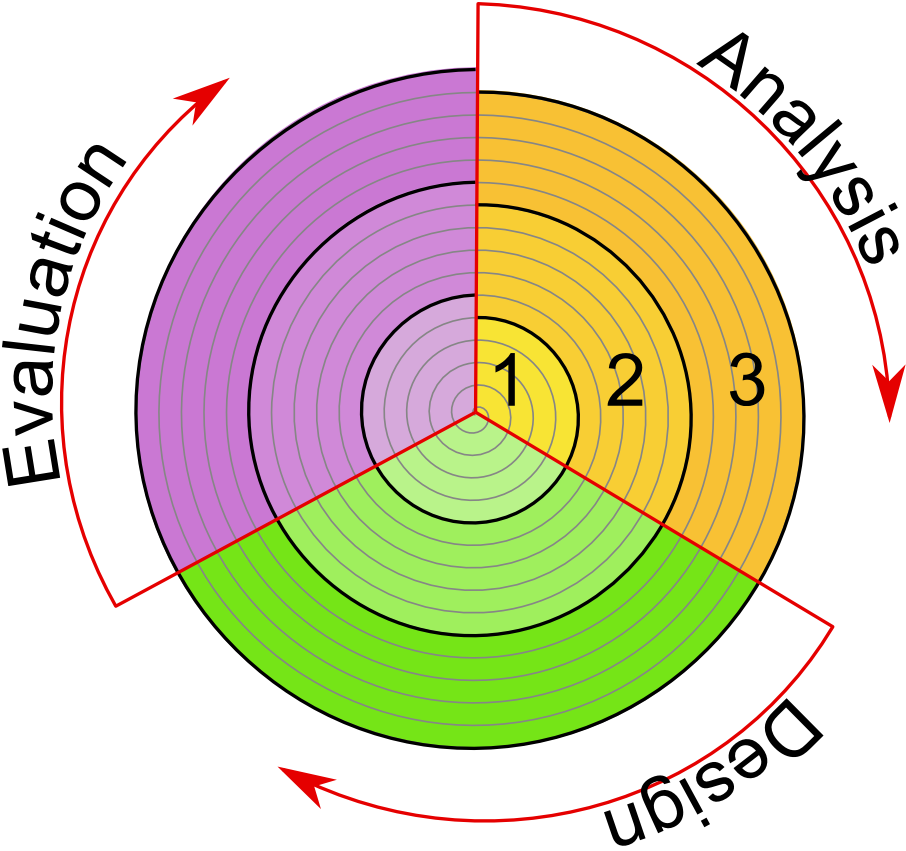
\includegraphics[width=0.5\textwidth]{espiral2.png}
\caption{ \label{intro_spiral} The user centered design process}
\end{figure}

During the analysis phase, all the information gathered from the subjects should be sorted and analyzed. Patterns and common needs should be made evident, and design decisions should be made based on these observations. It is crucial that the proposed solution respects current standards and that it integrates well with current tools. Designers should also implement the language used by final users instead of the technical terms used inside.  Proposed functionality should manifest as prototypes which may then be used for the evaluation phases. The users are engaged again in order to assess if the design is on the right track and the necessary adjustments are being made. During this process additional questions or use cases may emerge, potentially motivating the need for additional information from users. All of this information becomes input for the next iteration.

%Respect standards
%Play nice with current tools
%Language of the users
%Cite UX-book
%Be a listener
%Users hide ignorance, thy try to appear smart

\section{Objectives}

This thesis addresses the challenge of developing tools for supporting exploratory analyses with cohort data, applying the principles of visual analytics and human centered design. A model of how data and analysis tasks interact in a typical exploratory scenario is used as the foundation for the design and development of a tool to facilitate exploratory analysis of brain data. Using this model and a user-centered design process with practicing neuroscience researchers, a prototype tool called BRAVIZ is developed. To evaluate the prototype it was used in a large study, and it had a significant impact of how researchers use their data. In summary, objectives of the thesis are:

%Objectives
\begin{itemize}
\item Create a model of cohort data and visual analysis tasks that can be used to guide the design of exploratory analysis tools for cohort data.

\item Implement a prototype based on the model to validate it in the brain studies case.

\item Evaluate the prototype with a real brain study, real users and real tasks.

\end{itemize}

The research focuses particularly on multi-disciplinary teams of users. These teams generally include people with a wide variety of expertise such as radiology, imaging physics, physiology, neurology, cognitive psychology, statistical analysis, and many others. In addition, such teams are generally interested in looking at each subject's data as a whole, instead of looking at each data source independently. Interactions within and between the different specialists are considered inside the model.

%Hypotheses
The working hypothesis is that  current tools are not ideal for exploratory analysis of cohort brain data. Exploratory analysis is more efficient when only specific functionality is exposed to the user and the rest is handled automatically, without user interaction. In particular repetitive tasks and complexities in data access are barriers.

In order to assess this need it is necessary to determine several aspects and priorities of the neuroscience research community. How often is exploratory analysis done? If not often, then why? How can it be made more efficient? How can it involve more people? What are the main bottlenecks that limit exploratory analysis? This work addresses only the technological bottlenecks, but certainly other types exist, for example cultural or political. The ultimate goal of this work is to make exploratory analysis more viable, which in turn means making better use of the data and thus encourage more researchers to adopt reproducible research practices, open data, open source software, and in general, facilitate a more collaborative model for science.

%Research questions


%What are the requirements for visual exploration in cohorts?
%What are the most important tasks?
%What is the appropriate level of detail?
%How can multiple points of view be supported?


\chapter{Related Work}
\label{chap_related}

Structure

Exploratory Analysis + Large datasets  = Visual Analytics
+ Image Brain Data => Visual Analysis of Brain Data

\section{Exploratory Analysis}

%Difference from confirmatory analysis
%We need both
%Hypothesis generation
%Main elements of exploratory analysis
%Visualization plays an important role
%Pertinent today, data explosion, open data
%
%Tukey
%Wickham : let data surprise us
%Human Brain Project
%Connectome
%Open Data
%Hypothesis Generation


Confirmatory statistical tools are useful for looking if data supports a particular a hypothesis or fits to a particular pattern.  During confirmatory analysis researchers look at data in a systematic way in order to find answers to questions raised based on previous knowledge. This methods can answer these questions, but it does not leave any room for surprises or for finding the unexpected. Also, sometimes researchers are faced to data sets from which few is known in advance. Analyzing a data set without a clear question or hypothesis requires a completely different approach. ``Finding the question is often most important than finding the answer''\autocite{tukey_we_1980}.

Exploratory data analysis is a methodology for learning and understanding data without the need for previous hypotheses or questions. It seeks to let data talk, and let the researcher understand what the data is showing about the world. Exploratory analysis techniques include descriptive statistics, but the most productive methods are based on data visualization \autocite{tukey_exploratory_1977}. If information is presented correctly, the human eye can instantaneously perceive patterns, trends, and oddities. However, usually one does not know in advance what is this correct way to represent the data, and therefore usually exploratory analysis requires trying different representations. ``Examples of interesting results are anomalies (data that not behave consistent with expectations), clusters (data that has sufficiently similar behavior that may indicate the presence of a particular phenomenon), or trends (data that is changing in a manner that can be characterized and thus used for predictive models)'' \autocite{ward_interactive_2010}.
These kind of analyzes can raise hypotheses, which should be tested using tools from confirmatory analysis. Therefore both methods complement each other.

It is well known that the amount of data available for analysis is growing every day. Large amounts of data are available through social networks and government open data initiatives. Also several large research efforts are making the acquired data publicly available (For example the alzheimer's disease neuroimage initiative \autocite{jack_alzheimers_2008}, and the human connectome project\autocite{marcus_human_2013}). These data sets provide an opportunity and a need for large scale exploratory analysis. ``Secondary use of large and open data sets provides researcher with an opportunity o address high-impact questions that would otherwise be prohibitively expensive and time consuming'' \autocite{viangteeravat_giving_2014}. At a smaller scale, research groups are now able to acquire more data from more subjects. This data is often used in confirmatory analysis, and afterwards many groups are making the data available for exploratory research. 

\section{Visual Analytics}

%What it is?
%Why?
%Data 
%Data acquisition + transformation
%Humans and computers
%Automatic Analysis and Visual Analysis
%
%Jim Cook
%Keim

Visual Analytics emerged as a response to the challenge of making sense of large amounts of heterogeneous data. The term was coined by Jim Cook, who proposed a research agenda on the field in the book \emph{Illuminating the Path} \autocite{cook_illuminating_2005}. This discipline is located at an intersection between data management, data mining, scientific and information visualization, perception and cognition, and human computer interaction \autocite{keim_visual_2008}; and its main contribution is that it recognizes human domain experts as the most important actor in extracting meaning from data.
``It is indispensable to include humans in the data analysis process to combine flexibility, creativity, and background knowledge with the enormous storage capacity and the computational power of today’s computers.'' \autocite{keim_visual_2008}

The core of visual analytics is creating environments where human experts can work efficiently with high performance computers.
``The science of visual analytics must be built on a deep understanding of how
people sense, reason, and respond. This understanding is essential if we are to create
tools, systems, and processes that complement the strengths and compensate for the
weaknesses of the human beings involved.'' \autocite{cook_illuminating_2005}

This efficient interaction between human experts and computers is achieved through the use of rich interactive visualizations and fluid interfaces. The human visual system is recognized as the most efficient channel for transferring information from the computer to the expert's mind, and at the same time it is a natural pattern finding machine. Computer systems supporting visual analytics must be able to manipulate large amounts of data rapidly in order to keep up with the human expert. Processes that take a long time should provide intermediate visualizations and give the expert the chance to steer them or cancel them if they notice they are not going in the right direction. Results obtained through expert interaction are immediately understandable, while those obtained by machine learning require an important interpretation effort \ref{stahl_overview_2013}.

Daniel Keim presents the visual analytics process as several iterations of data transformations, automatic data mining, model refinement, data mapping to visual representations, model building, model visualization, and user interaction \autocite{keim_mastering_2010} (see figure \ref{fig_workflows}-b). This thesis is focused on the area of data visualization and user interaction to support visual analytics on data from brain studies. Data transformation and data mining will be done using third party tools.

The discipline of visual analytics is still young, and there are still several challenges that need to be solved, specially towards making it available for the general public\autocite{kwon_visual_2011}. Since the book by Jim Cook there has been significant interest in visual analytics research \autocite{chen_illuminated_2012}, and more tools have become available. Likewise, there has also been important developments on all the areas that support visual analytics. At the same time there is an increased interest from governments and organizations to extract value from data. All these indicated that visual analytics will continue growing and become a big player in business, government and research.


\subsection{Interactive Visualization}

%Difference from standard visualization
%Perception
%Clean / easy to grasp
%Interaction
Interactive visualizations are one of the main supporting elements of visual analytics. Bertin 
\autocite{bertin_graphics_1981} introduces two different types of graphics, ones used for communicating information, and others used for graphical processing. This thesis will be focused on the second type, but notice that Jim Cook recognized information dissemination as an important component in visual analytics \autocite{cook_illuminating_2005}.

% General graphical representation

Representing data statically efficiently requires significant attention to details. One of the most important works in the are is \emph{The Visual Display of Quantitative Information} \autocite{tufte_visual_1983} , by Tufte. It emphasizes that data should be the center of the visualization, and additional elements should be kept at a minimum. For example, labels in axes should correspond to the values of the data, instead of arbitrary \emph{round} numbers. Graphical elements and decorations that don't add anything to the understanding of the data (ducks) should be avoided. It is also important to keep in mind how the human brain perceives elements, and therefore avoid unnatural representations. For example, one should not map values to volumes in a paper or a computer screen. He also introduces small multiples displays as a way of efficiently comparing multidimensional data. In this representations full displays of each point are represented are displayed next to each other, all at the same scale and with the same set of visual parameters. This allows users to focus directly on the data, and don't worry about individual representation characteristics of each image.

It is also important to consider aspects of human cognition. For example consider that the visual system is much more sensible at discriminating lengths and positions than at discriminating colors or angles \autocite{ware_information_2004}, therefore the most important information should be encoded using position or length. Additionally, the visual system capable of correctly discriminating between seven different colors or shades of grey \autocite{miller_magical_1956}.



% Unique to interactive graphics

Interactive visualizations should allow specialists to think based on them. This means, that the interactions should match with the thought processes going on during data analysis. A good description of this process is described in the data visualization mantra ``Overview first, zoom and filter, details on demand'' \autocite{schneiderman_designing_1998}. \autocite{yi_toward_2007} provides a taxonomy of user intentions when analyzing data trough interactive visualizations, where such systems are characterized by the fact that information from the system to the user is much larger than from the user to the system. The proposed taxonomy seeks to be descriptive (captures most user intentions, and permits easy classification of new techniques), evaluative (can help to analyze if a system is helping the user) and generative (can help in the design of new systems). The intentions included in the are the basis for the enumeration of analysis tasks in chapter \ref{chap_model}.

In \autocite{ware_information_2004} Colin Ware reviews perception issues affecting how images are understood in the brain. It also explains how interaction can be used to think about data. He insists on that ``the cognitive impact of the interface should be minimized, so that thinking is about the problem and not the interface''. The eye can move jump instantly from one position to another, while moving a mouse requires time. Switching to another windows by moving the eyes is much faster and easy than by using the mouse. According to Ware, ``the best visualizations are not static images to be printed in books, but fluid, dynamic artifacts that respond to the need for different views or for more detailed information''

Several design patterns for visualization applications focused on the interaction between the computer system and the human cognitive capabilities are described by Ware in \autocite{ware_visual_2013}. He represents the system a machine where objects can be moved from the expert's working memory to the computer memory and viceverza. In a similar way problems can be solved by visual pattern search using the expert's visual system or by using the processor in the computer. Also moving the eye to a different area of the screen (or a different screen) is much faster than changing the visualization in the computer. The objective is to make the best possible use of this resources for the given application. 


A review of visualization techniques can be found in \autocite{heer_tour_2010}. It emphasizes that visualizations should consider the natural strengths of the human visual system to see trends, patterns and identify outliers. \autocite{heer_interactive_2012} complements this review with techniques for interactive visualization. It is recommended to provide several linked views of the data, and allow connection between them. Systems should also work at the same speed as human reasoning does (fast). It is important to provide mechanisms to filter data and see more details of interesting data points. It is also convenient to include basic statistical functions to avoid making the user change to a different program, which would cause a disruption on the workflow. Likewise, maintaining a history of the analysis allows specialists to review the steps that lead to a certain point, and to go back and take detours in the data analysis. Having the option to undo all actions allows the specialist to take more risks and therefore move faster in the analysis. This history works better if it can be annotated to reflect what was going on in the specialists mind at different points. These mechanisms can also foster collaboration and sharing of information between members of a group. Communication between members of the group is more efficient if all members have access to the same visualization, even if they are physically at different places.



%\autocite{fayyad_information_2002}	Information visualization in data mining and knowledge discovery (en la biblioteca, pg 9 revisión biblio)

%\autocite{spence_information_2007} provides an overview of the challenges and strategies present in interactive visualization settings.

%\autocite{card_structure_1997}	more examples of interactive visualizations. 	

%Research on the theoretical aspects of data visualization \autocite{purchase_theoretical_2008} tries to better understand the factors that determine if a visualization is effective, and in this way predict which visualizations would be the most effective for a certain task and user.
	

\subsection{Visual Analytics Examples From Other Domains}

Data acquisition and visualization methods have rapidly evolved in the past years \autocite{botha_individual_2012}.

Examples : 
Document Analysis: Inspire \autocite{hetzler_analysis_2004}, Atlas TI, Theme River \autocite{themerivertm:_2002}
Military: Strategic airlift \autocite{soban_visual_2011},
Chemical Industry: \autocite{stahl_overview_2013}
Multi-attribute ranking LineUP \autocite{gratzl_lineup:_2013}
Public Health: \autocite{sedig_challenge_2014}
Science policy: \autocite{mcinerny_information_2014}
Electricity consumption \autocite{janetzko_anomaly_2014}

\subsection{Evaluation in Visual Analytics}

Hard problem
Different techniques
Different stages

\autocite{munzner_nested_2009} describes a model of the different levels at which it is possible to make contributions in data visualization, and the correct approaches to validate claims at each level. It goes from low level algorithm design where measuring computational performance is the correct approach, to domain problem characterization where validation consists on observing adoption rates and interviewing target users.

Los del test con Ana
Schneidermann.... long term in depth...


\section{Tools for Visual Analysis of Tabular Data}

R  / stata  / python
prism / spss / stata
ggobi
ggplot \autocite{wickham_practical_2008}
ggvis
shiny
deducer
tableau
aabel
d3

\begin{table}
	\centering
		\begin{tabular}
			
		\end{tabular}
	\label{tab_related_tabular_applications}
\end{table}


%--------------------------------------------------------------------------------------
%--------------------------------------------------------------------------------------
%--------------------------------------------------------------------------------------


\section{Neuro-Image Analysis Techniques}

Basics of images, voxels, coordinates, scalars


\subsection{Registration}

FSL
ANTs
SPM-Dartel


Comparing two different brains is a challenging task, specially in the cortex where the pattern of folding between two subjects can be substantially different \autocite{toga_new_2002}.

\subsection{Structural Images}

SPM
FreeSurfer

Segmentation

Segmentation of hippocampus, robust in presence of pathology \autocite{kim_robust_2011}.

Shape analysis

SPHARM

\autocite{hermann_visual_2014} propose a system to interactively explore shape variations between a structure from different subjects or at different times. The system provides three different visualizations at different levels of detail. The first view shows the overall pattern across the structure, the second one allows the user to focus on a substructure and see how changes on it are related to the rest of the structure, and the final one lets the user interactively modify the structure by dragging a  point and see how the rest of the structure would be modified. 

\subsection{Functional Magnetic Resonance}

SPM
FSL
AFNI
Handbook of fMRI

BrainVoyager \autocite{goebel_brainvoyagerpast_2012} is a commercial package for high performance processing of functional, diffusion and structural brain data. Its algorithms are optimized for producing fast results (some even realtime), by using all of the available hardware. It includes a scripting language for analyzing bulks of images, and it is also incorporating the newest techniques as Multi-Voxel pattern analysis, a machine learning technique for inferring the state of the mind based on data from functional imaging and a previous training. By doing this analysis in real time it can be used for brain computer interfaces. 

\subsection{Diffusion Weighted Images}

CAMINO
DIFFUSION TOOLKIT
TRACULA



Several software packages are available for processing diffusion weighted images \autocite{hasan_review_2011}

Reconstructing fibers that cross each other, or fold in tight angles is a hard problem \autocite{fillard_quantitative_2011}, and specially tensor based methods are not able to deal with them \autocite{tournier_diffusion_2011}.


\autocite{blaas_fast_2005} presents a method for isolating fiber bundles by defining several regions of interest. Internally bundles are organized in a KD-Tree which permits interactive selection.

\autocite{goodlett_group_2008} proposes a method for performing statistical analysis of white matter, by constructing a representative fiber bundle of the population understudy, mapping it back to the diffusion image of each subject and sampling scalar values from it. In this way statistics can be performed along the tract, with scalars taken equivalent locations on each subject.

\autocite{colby_along-tract_2011} proposes analyzing scalar values along the fiber, instead of extracting just one number that represents the whole bundle, this allows finding patterns that relate to specific pieces of a white matter way.


TBSS \autocite{smith_tract-based_2006} is another approach for analysis of diffusion data. Its main characteristics is that images from different subjects are co-registered based on the structure of white matter. 

\subsubsection{Tractography Clustering}

\autocite{song_zhang_identifying_2008} explore two methods for clustering fiber bundles, in the first one fibers are assigned to the same cluster if they are sufficiently close, while the second one tries to optimize a global measure of separation between clusters.

\autocite{guevara_automatic_2012} presents a method for clustering the main pathways on massive tractography datasets based on an atlas composed of common pathways in a group of subjects, and manually labeled by experts. This atlas can afterwards be used to isolate these bundles on new brains.

\subsubsection{Connectivity Networks}

\autocite{rubinov_complex_2010} presents several methods for building networks from MRI data, and how graph theory metrics can be applied and interpreted in such networks.

\autocite{li_visual_2012} introduces a software for robust construction and analysis of brain networks. In this software local diffusion or functional features are calculated at the position of each node, then the system tries to find the best position for the corresponding node in different subjects by minimizing the differences of these local features.

In \autocite{richiardi_decoding_2011} a system for decoding the state of the brain based on the fMRI connectivity graph at different frequencies.

\autocite{alper_weighted_2013} studies visual techniques for comparing two weighted brain networks. The tool is based on a research of analysis tasks common in brain network research. At the end two visualizations are recommended based on a user study; one of them is very good for small networks while the other performs better in networks with many nodes and edges.

\subsection{Spatial Data Visualization}

3D Slicer
FreeView / TkView
BrainVisa
Osirix / PACS / Proprietary
VTK / PARAVIEW
MRICRON / ITKSNAP



%---------------------------------------------------------------


%-------------------------------------------------------------------
%In \autocite{paus_mapping_2005} a meta study about brain development is presented. It makes the point that by looking at different modalities of information in an integrated way is useful for making better assessments of intersubjects variance. He also mentions the potential from alliances between image experts with social scientists, geneticists and mental health professionals.

%\autocite{lenroot_brain_2006} analyzes the development of adolescents brain based on about 4000 scans of 2000 subjects. It makes use of manual and automatic techniques for registration and segmentation.

%\autocite{konrad_vbmdti_2012} presents a study that integrates local diffusion and structural features from the Broca area to results in a verbal intelligence test. In their discussion they mention that it is hard to specify the direction of this relation, this is, if a the structural difference causes a difference in performance, or if learning of verbal skill causes a change at the structural level. 


\section{Visual Analytics for Brain Images}

\autocite{bezgin_matching_2009} presents a tool for exploring data of the macaque brain. It uses an onthology and an atlas to query spatial features and connectivity, and connects to the \emph{cocomac} database which contains data from several studies. "Comparison between studies provide more meaningful insights than each study alone".

IRaster \autocite{somerville_iraster:_2010}  is a tool for visualization and analyzis of electrical signals acquired from high density intracraneal micro-electrodes. Integrates several known signal analysis methods with interactive visualizations which supports deciphering several spiking patterns.

\autocite{steenwijk_integrated_2010} presents two integrated tools, one for processing of image data in order to extract features, and one for interactively visualize and explore such features. Visualization is achieved through scatter plots and parallel coordinates plots, using techniques such as brushing and coloring by a different variable.  Given one point in the exploration, the tool allows the user to find the raw data that originated it. This system is presented as a tool for hypothesis generation. 

Invizian \autocite{bowman_query-based_2011, bowman_visual_2012, van_horn_graphical_2013} provides a representation of multiple brain scans in a "Feature Similarity Space", where all brain surfaces are located in a 3d space in such a way that \emph{similar} brains are nearby. The similarity metric can be defined used several scalar features calculated from each brain. The system also integrates with ggobi to combine the spatial analysis with interactive analysis of scalar data.

\begin{table}
	\centering
		\begin{tabular}
			
		\end{tabular}
	\label{tab_related_brain_applications}
\end{table}

\chapter{A Model for Exploratory Brain Data Analysis}
\label{chap_model}
%Introduction

The human brain can be analyzed from different points of views. Some disciplines look at it from the outside, and try to understand how it responds to stimuli, how it behaves on different conditions, how it adapts to new contexts and how it changes over time. Some disciplines look at it at cellular and molecular level, trying to understand the chemical reactions that go on inside each cell making it work. Others analyze the activity of a groups of cells analyzing how they cooperate. Some focus on larger structures composed of several cells, trying to understand how they connect to each other and how the different types of organs complement each other. It is of special interest seeing how it matures over time, and how it recovers from traumatic events. Additionally it is important to analyze how it degenerates over time, and what diseases can affect it in order to create treatments and help the brain heal. 
These tasks are carried out by different specialists in very different environments. There are also a wide range of tools designed for studying the brain, from microscopes and voltage clamping techniques, to psychology instruments. There are also studies based on animals with similar structures or even electronics circuits specifically built to emulate the human brain. 

This shows that understanding the brain is far from easy, and that it involves an enormous amount of skills, tools and knowledge. It can also be seen that all of these information gathered from different perspectives must be integrated in other to get a full understanding. This will require teams from diverse specialties and contexts to work together, each providing one piece of the puzzle. 

This task will also require support from computational tools in order to be efficient. These tools should allow experts from different contexts to be productive as teams and to integrate data acquired using a wide array of methods. Data itself will be highly heterogeneous and there will be lots of it. As tools advance we become more efficient at making experiments and generating data, and the bottleneck has become analyzing it. In other words, data is acquired at a fastest rate than it can be understood. 

This is indeed a complex scenario, and it is evident that a single software tool will not be able to solve all the problems. Tackling the whole problem at once is also an impossible tasks. We need to break down the problem into simpler tasks that can be attacked without loosing the big picture. Doing this analysis is itself a challenging task, that can't be addressed lightly. Fortunately this kind of problems are found in several business applications and  software engineering techniques that can manage them have been developed. 

As mentioned previously, the problem of integrating brain data involves several points of view and several types of work-flows. This is a clear signal of the need for different applications instead of a single, all-mighty application. Nevertheless these applications will likely share several aspects. Analyzing these commonalities and differences is the first step towards a solution to the problem. 
Methodologies to do this can be borrowed from software product line engineering \autocite{pohl_software_2005}, model driven software engineering \autocite{brambilla_model-driven_2012} and generative programming \autocite{czarnecki_generative_2000}. 

The first task will be the scoping of the domain and the selection of a domain where a it is feasible to make a contribution. Afterwards the commonalities and differences in the needs of the different stake-holders, work-flows, and data in the selected domain are analyzed in order to create a feature model. This model will be the basis for a proposal of an applications family, where each application addresses a particular problem inside the domain. 


\section{Domain Engineering}

Domain Engineering is the practice of selecting and characterizing the domain in which the application family will be built. A good description of the steps required for this task can be found in \autocite{czarnecki_generative_2000}. We will follow these steps in order to identify the domain where we will work on the rest of the thesis.

\subsection{Domain Scoping}

As noted previously brain research involves several specialties, skills and techniques. It could be argued that because the brain is involved in almost every human action, all human and social sciences are at the end studying the brain. However in this project we will focus on more direct studies of the human brain. In particular we want to analyze its physical structure. Under this condition there are still a broad ways of looking at it.

In domain engineering the decision of where to focus must be also influenced by the strengths and experience of the organization, in this case our research group. Previous projects of the group (\footnote{Proyectos de Darwin, Jaime, Marcela}) have principally focused on analysis of medical images at m.m. scale, acquired by CT and MRI machines. We have good relationships with radiology departments at several hospitals and therefore access to images and, more critical, domain experts. MRI is an specially interesting technique as it does not produce ionizing radiation, and therefore is harmless for the subject. While CT and general x-rays involve radiating the human body. This is not harmful at small doses but the effects may accumulate over time. Therefore these techniques must be used with care and only when there is a valid medical reason that justifies it. On the other side, MRI scans can be applied to any subject and there is no need for a medical justification (but probably the study must be approved by an ethical committee). MRI scanners are also versatile machines which can acquire numerous kinds of images. Structural images can be acquired at different configurations which provides better contrast for different tissues or molecules. Advanced techniques grant the ability to do spectroscopy in order to characterize the composition of specific areas of the brain. By using contrast agents it is also possible to precisely locate specific proteins, cells or structures. 
For these reasons we chose to focus our development on images acquired by MRI. We also chose to focus on T1 and T2 weighted structural images, Diffusion weighted images and BOLD f-MRI. This decision was also caused by the previous experiences in the group, but nevertheless keep in mind that domain definition and scoping is an iterative process, and therefore this decision will certainly be revisited in the future.

An objective of the project from the start has been the integration of data, therefore even though we are focusing on MRI data, we need additional data to provide context and therefore a more complete picture. Recall that one of our hypotheses is that the brain is better understood by teams of specialists who can bring different perspectives. One of our challenges was linking structure and function of the brain. This function of the brain may signify quick reactions to stimuli, like for example catching a ball, all the way to complex social behaviors over several years. This kind of data can be collected by economists, psychologists, epidemiologists, and sociologists among others. This information can be very complex, but a non trivial subset of it consists of numerical, nominal and ordinal variables which can be registered in spreadsheet tables. We will attempt to integrate data from these diverse set of disciplines if it is presented in a table-like format, but we will not try to interpret the data in any way. This responsibility will fall on end users. 

Finally there is another important kind of data we want to consider as it provides a perfect link between structure and functioning of the brain. This is, data from TMS exams. We are very lucky to have access to neurophysiologists specialized in this kind of exams, which can further enlighten the functioning of the brain and its relationship to its structure. To recapitulate, the current project is going to consider the following kinds of data:

\begin{itemize}
\item MRI brain images
\begin{itemize}
\item Structural T1 and T2 weighted
\item Diffusion Weighted Images
\item Functional MRI
\end{itemize}
\item TMS exams
\item Tabular data from other disciplines
\begin{itemize}
\item Nominal variables
\item Ordinal variables
\item Numeric variables
\end{itemize}
\end{itemize}  

Another key aspect of domain scoping is identifying stakeholders and their interests. As mentioned earlier the brain can be studied from a clinical perspective with the aim of healing it. This is usually done case by case in hospitals or health centers. While this is a very important activity, we are most interested in analyzing cohorts of subjects. Also, getting into the clinical diagnosis practice would involve dealing with significant more regulations, which would increase the complexity of the project. The other major group of users of medical images are brain researchers. As was described in the introduction chapter, this is our main target. In particular we focus on interdisciplinary brain research projects, where there is data from multiple subjects and different nature, and an interest to find relationships across the different dimensions. The data available for each subject should be reasonably consistent across the complete sample. The stakeholders are therefore the researchers involved in such a project. These researchers can come from several backgrounds, which include

\begin{itemize}
\item Radiologists
\item Physicians
\item Psychologists
\item Physiologists
\item Epidemiologists
\item Economists
\end{itemize}

Their goals are extracting information and meaning out of the data. As mentioned earlier this is the core problem that lead to the birth of visual analytics. However it is crucial to understand that each specialist will inevitably have his own interests and his own methods. The real challenge is creating a common framework that would help and encourage specialists from different disciplines to work together and collaborate efficiently. Therefore in order to achieve the ultimate goal it is necessary to improve communication inside the team, and to encourage specialists to go out of their zone of comfort and ask questions about data they don't usually look at. However this must be done responsibly, the objective is not to ignore the true specialists in a particular kind of data, but the opposite, improve communication between these specialists. 

Each specialty also incorporates their own work-flows. These include protocols for data acquisition, pre-processing, storage, processing and analysis. As mentioned in the introduction analysis usually take the form of null hypothesis significance testing, and plenty of tools exist for this purpose. Nonetheless exploratory data analysis is also very important, specially when huge amounts of data are available. Traditionally data acquisition was also tuned for the testing of particular hypotheses, but it is becoming common to acquire data in a more open-ended fashion. In this project we will not deal with data acquisition nor data processing. The focus is on visual exploratory analysis of already processed data.  

In conclusion, the scope of the project is now bounded in data types (MRI and tabular), stakeholders (interdisciplinary research groups), and tasks (visual exploratory analysis). However, it is worth reiterating that domain scoping is an iterative process, which has to go on for the duration of the project. 

Domain Model

%- Stakeholders
%- Users
%-- points of view
%-- activities
%-- teams
%-- selfish
%
%-- Alternatives
%-- choose
%- Scope
%-- Alternatives
%-- Choose


\subsection{Domain Modeling}

After choosing and bounding the domain we need to go deeper into its characterization. This task is accomplished by reading bibliography in the domain, contacting stakeholders and analyzing existing software. The details of the information gathered at this stage can be found in chapter \ref{chap_related}. In this section we will describe the domain based on that information.

%Workflow
A typical MRI experiment starts with a set of hypotheses which want to be tested on a target population. A protocol is designed to test the hypotheses and if possible correct sample sizes are calculated. Afterwards participants are recruited, and data is collected. This process is not always smooth, and often corrections must be made and acquisition repeated. Inevitable some data will not be useful and some participants will have to be removed from the study. Data acquired from the MRI machine must be taken out, stored and processed. There are different processing pipelines for different kinds of images, but most of them are designed to perform statistical tests using the images and some external variables. The results of the statistical tests have to be interpreted in order to write the report of the experiment and what we learned from it.

As mentioned in chapter \ref{chap_intro} we intend to use data collected in these experiments as well as data collected in open-ended fashion to perform exploratory and data-driven analyzes. Still, most of the steps in traditional experiments will be the same, and we are required to play nice with existing tools and work-flows. 

\begin{figure}
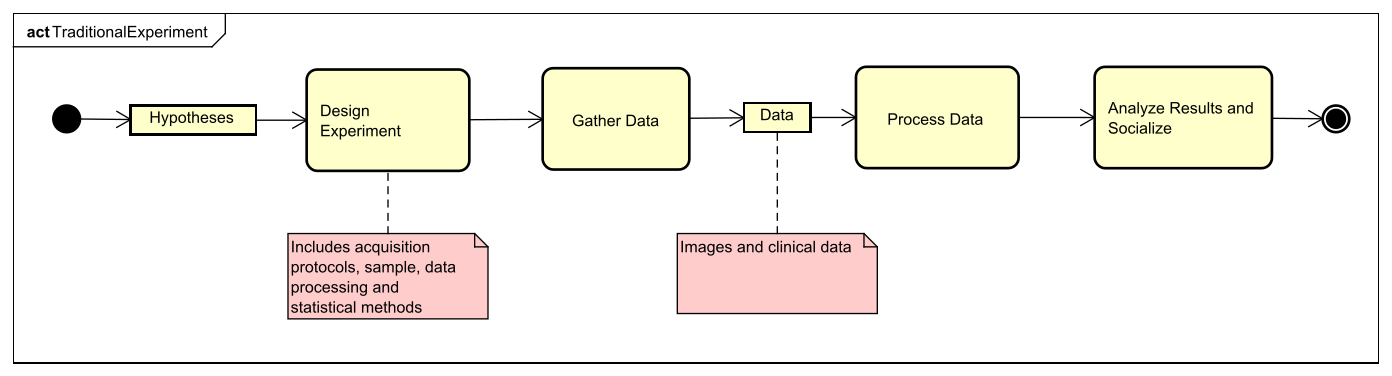
\includegraphics[width=0.9\textwidth]{Figures/domain/TraditionalExperiment}	
\caption{\label{fig_workflows}}
\end{figure}

Figure \ref{fig_workflows} shows the comparison of the two work-flows. It can be seen that the input for traditional experiments are hypotheses, while the output of data driven research are also hypotheses. Meanwhile the input to the data-driven research loop is data, which as mentioned earlier can come from finished experiments. This shows how both work-flows can complement each other. Also notice data processing takes place at both loops. The meaning is that the data-driven and hypotheses-driven research domains are deeply linked.  

%Data
\begin{figure}

\caption{\label{fig_datum_class}}
\end{figure}

Data is the most important object in our domain, so we need to characterize it in a more precise way. Inside our scope, data is a collection of data-points each of whom is also called a datum. Figure \ref{fig_datum_class} shows a class diagram of a datum. The highlights of the drawing are

%definitions

\begin{itemize}
\item Each datum is associated to an Entity
\item An entity may be a single subject or a sample
\item A sample is composed of several subjects, each subject can belong to several samples
\item The two main kind of datum (in our scope) are spatial and variable values
\item An spatial datum may be an image or polydata
\item All spatial objects are associated with a coordinates system
\item Transforms can be used to map between two coordinate systems
\item Images are composed of voxels
\item Polydata are collections of vertices, edges and polygons
\item Voxels, edges, vertices and polygons may be associated with one or more scalar values.
\item All spatial data must me associated to some meta-data
\item VariableValues belong to a certain variable
\item Each variable is associated with meta-data  
\item Data which is neither a VariableValue nor a spatial object can be encoded into textual annotations
\end{itemize} 

Meta-data plays an important role. On the spatial side it lets us identify which images or polydata can be analyzed together. In other words, it is through this metadata that it becomes to possible to identify matching pieces of information belonging to different subjects. In the case of variables, the metadata provides important information on how to interpret the values that the variable takes. Some concrete examples of data are
\begin{itemize}
\item Image:
\begin{itemize}
\item T1-weighted structural image
\item Color coded DTI image with 3 scalar values per voxel
\item A label map where each voxel contains a value indicating to what structure it belongs 
\end{itemize}
\item PolyData:
\begin{itemize}
\item A group of fibers from a tratography
\item Cerebral cortex surface reconstruction
\item An iso-surface representing an activated area in a fMRI paradigm
\end{itemize}
\item Variable:
\begin{itemize}
\item Gender
\item Height
\item Score at a neuropsychological test
\item Time it took to complete a marathon
\item Level of pain in a likert scale
\item Place of birth
\item Latency in a TMS test
\end{itemize}
\end{itemize}

%Processing

It can be seen that this simple structure allows us to represent a wide array of data types. Some of this data are raw values that can be found directly, and some are the results of processing steps applied to raw data. As mentioned earlier we don't expect our system to do data processing, but there is a close relationship with these kind of procedures. In fact the system should be able to do additional processing when it is required, but delegating this task to third party tools fit for the job. As seen in figure \ref{fig_workflows} processed data is fed back into the system, and afterwards can be used in the same way as raw data. Some examples of the processing steps that we expect to utilize are

\begin{itemize}
\item Estimating diffusion models (like DTI)
\item Reconstructing tractographies
\item Segmentation of structural images
\item Reconstruction of segmented structures
\item Cortical surface reconstruction and parcellation, as done in FreeSurfer
\item Linear and non linear registration
\item Applying transforms to move spatial objects to a different coordinate system
\item Creating frequency maps from several co-registered label maps.
\item Filtering tractographies
\item Calculating volumes, areas, and mean values of a scalar, for a given surface.
\item Statistical tests involving images from two different groups (like VBM, or second level fMRI analysis)
\item Clustering on a set of variables
\item Fitting of statistical models on a set of variables
\end{itemize}

As usual, this is not an exhaustive nor final list. As the project evolves it is likely that we will have to incorporate additional processing algorithms. The vision is to take advantage of available tools whenever possible. Fortunately there is an ample set of high quality open source tools available as was shown on chapter \ref{chap_related}.

%Stake Holders

The expected users in this project are research groups containing specialists from different backgrounds, however there are several other stakeholders who must be considered in the development of the project. The data comes from real participants, which may have concerns about too many people looking at their data. On the other side the project managers and funding agencies want the best return of investment possible, which means extracting as much information and knowledge as possible from the collected data. Usually the participants of the experiment, whose data was collected, signed a consent which permits some use of the data. The contents and permissions granted by these agreements have to be taken into account. A common trade-off is for the participants to grant unlimited usage of the data as long as it is anonymized. In theory it shouldn't be possible to figure out the true identity of a subject based on anonymized data, but this is hard to guarantee in practice, specially when so much complementary data can be obtained from third parties \autocite{singel_netflix_2009}. Also the anonymization procedure involves adding noise to the data, which will have an impact on the analysis. When data is analyzed as extensively and deeply as we are proposing, the risk of deanonimyzing the subjects increases. Therefore measures have to be taken into account to increase protection, either by limiting access to the data to a small group of researchers, or increasing the strength of anonymization measures. 

Another possible concern is the loss of statistical rigor. As shown in figure \ref{fig_workflows} traditional research is based on the fact that data is used once for a statistical test. In this case meaningful metrics of significance can be reported. However when data is used more than once we fall into a multiple comparisons problem \footnote{quote}, where the chances of false positives increase and therefore corrections should be applied to significance metrics. Nevertheless the scientific community is concerned that researchers will not apply corrections and report results which are not really accurate. While we can't do anything against dishonest researchers, the proposed platforms may make it easier to cheat in order to get more impressive results. As mentioned on the introduction, this problem arises from publication bias. Under this situation some researchers may believe that the best way to guarantee a publication is by reporting some fantastic significance metrics, and try everything they can to get this values. It is key here to remember that the proposed platform is meant to be used as a mean for generating hypotheses, not to formally proof them. While the analysis carried on in the platform may provide evidence in favor of some hypothesis, it is also highly susceptible to the multiple comparisons problems. Therefore it is necessary to be skeptical about the data, and always validate hypotheses using external datasets.  

Understanding the main users of the application is at the core of the design process. Recall that we are using a user centered design methodology, involving end-users constantly during the design process. Understanding the users is also central for the domain-modeling activity. This includes examining their current workflows and tools is the starting point for this. We accomplished this by visiting several labs and hospitals, and watching several experiments, from data acquisition to data analysis. The knowledge from other works in visual analytics can also be applied here. 

First of all, brain researchers are human. As humans we all have limitations on the amount of information we can keep in memory and our ability to concentrate. The analysis platform should help mitigate this by unloading the memory of the specialist to the screen. All of the required information should be visible or easy to access. In order to avoid distractions, it is important to have a fast response time. If the application constantly makes the user wait, then probably he will loose interest and move to another task. A peculiarity of brain researchers is that they are very busy, and usually there is no time in their agenda reserved for data exploration. This activity is carried on at the spaces between tasks, and even tough there is a high chance of being interrupted by students or colleagues. Therefore it is essential for the platform to support work at different intervals and under constant interruptions. In practice this means efficient facilities to save and restore work, as well as additional information to recover the flow from the last session. 

Visual Analytics recognizes that humans have limited cognitive capacity, and the point is to make the best possible use of it. One key point here is that the cognitive budget should be spent on the data and not on the tools. This means that the experts should always be thinking about the underlying data, not on details of the tool used to look at it. Consider for example watching TV, how much time do you spend thinking on details of the tv-set? If tools require complex commands, or the controls are not intuitive, the attention will have to shift to how to accomplish a task in the tool. Another key concept required here is that tools should adapt to users, instead of making users adapt to tools \autocite{norman_design_2002}. This also means that technical details or repetitive actions should be solved automatically. For example there are dozens of image data formats available, and each tool works with some of them. This forces the user to spend time thinking which tool is appropriate for each format, or if there is a need to convert it. The same goes to dealing with files in file system, users should not be thinking on what is the best way to organize files so that they can be easily found afterwards. 

On the other side, researchers are the most fit, if not the only, who can interpret and make sense of this vast amount of data. As the data grows larger, chances of patterns appearing by chance also increase. Only experts can discriminate between true interesting findings and random noise. They can do this because they possess a strong theoretical background, which can be used to give meaning to data. They also have experience working with patients and data, and therefore can associate data from a study to past experiences and close cases. From all these they have also developed an intuition, that can guide them to interesting places. Given the familiarity with the data, experts can quickly spot common mistakes or find simple explanations to what may appear surprising for an outsider. 

In summary some of the main characteristics of a hypothetical user are

\begin{itemize}
\item Limited memory
\item Limited concentration
\item Busy schedule
\item Not interested in technical details
\item Background knowledge
\item Experience
\item Intuition
\end{itemize}

%Group memebrs also belong to other groups

%Florero, evidencia de los argumentos, no recurrir a la memoria, sino tener la informacion visible

% groups

Groups of experts are also interesting because their expertise are on different areas. Therefore while they are deeply familiarized with some aspects of the data, other aspects are foreign. In a similar way each expert is inclined to analyze data of a particular nature or in a particular way. Some teams are composed of experts located far from each other. Often they don't even share the same mother language. Communication between the different members of the group is therefore challenging, as is reconciling their interests and objectives, and moving forward as a group. Communication is different when a link to the physical reality can be stablished \autocite{rojas_arredondo_dinamica_2010}. By having data easily available at a meeting, researchers can provide evidence to support their ideas, and in this way have a conversation rooted to reality, instead of relying on memory or notes. Also ideas or questions that come up during the conversation could be explored right away, which can lead to a more fluent and efficient work session. Visual Analytics recognizes the human visual system as the most effective channel to get information into the expert's mind. By using this channel efficiently we believe communication can be improved. Also by providing easy access experts, we may lower the resistance from experts to explore data from other fields by themselves, to follow-up with colleagues and bring them questions. Yet again, there exists the danger of some members of the group wanting to control their data, and don't liking the idea of non-experts looking at it because probably they will not understand it. We will have to wait and see how these kind of tools and environment affect group dynamics.


\bigskip

% Existing viualization applications
In chapter \ref{chap_intro} a review of the tools currently used in the domain was presented. These tools have several things in common and several differences as shown in figure X. While most of the processing tools provide utilities for batch processing several subjects, visualization are mostly available for a single subject or for the results of statistical tests. Going through visualizations of several subjects requires several steps and most of the time repeating work. Also while most of them permit the use of linear transform to move the data to a different coordinate system, the end user must specify the adequate transform for each case. These tools offer very good performance for quality control or publication graphs, but for exploratory analysis we require a more streamlined workflow, with minimal need for repetition, and limiting as much as possible the exposure of technical details to the user. In the world of statistical visualization there has been a bigger growth in interactive solutions. For example tableau can be used to create highly interactive dashboards for the exploration of large datasets. These dashboards display several coordinated views of the data and permit the user to interactively change parameters and therefore get visualizations tailored for the current question. We are interested in using these kind of techniques but extend them to be better integrated with spatial data. 

\bigskip

In summary, the target domain is characterized by
\begin{itemize}
\item Data Sources
\begin{itemize}
\item Spatial Data
\item Tabular Data
\end{itemize}
\item Visual Analytics
\begin{itemize}
\item Data Transformations
\item Fast iteration
\item Interactive Visualizations
\item Focus on data, not tools
\end{itemize}
\item Research groups
\begin{itemize}
\item Collaboration
\item Interrupted work
\item Diverse points of view
\end{itemize}
\end{itemize}

As mentioned earlier the objective is to create a family of applications that can adapt to different tasks inside the domain. Following visual analytics principle these applications should put the data at front, and let users focus on it instead of the applications. For this reasons applications should be simple, and have a limited set of features. Nevertheless we are also interested in fostering collaboration, and for these reason we would like applications inside the family to play nice with each other. It is also important that applications have strong features that let the user save and restore work efficiently, and therefore work over several interrupted sessions. Finally some applications in the family should support data transformation utilities. These transformations can be seen as measurements done based on spatial data, as well as additional geometric processing on spatial data, and the use of tools from the statistical analysis world. Visualization is the basis of exploratory analysis, and therefore it will likely be at the core of most applications in the family. The set of applications that will make part of the family can be better seen in the feature diagram of figure \ref{fig_feature_problem}.

\begin{figure}
\caption{\label{fig_feature_problem}}
\end{figure}

The main elements in the diagram are

\begin{itemize}
\item Application: The root of the tree, each of the applications in the family are configurated based on this tree
\item Visualization: Most applications will have visualization as its main component. The exception are applications that that only process data without interaction. Visualizations can exist for spatial data or statistical data.
\begin{itemize}
\item Spatial Visualization: These visualizations show spatial objects, these is, objects with coordinates associated to some physical space. Notice this visualizations can be in a plane, with only two coordinates, or a in a full 3d space. These visualizations can display one or several of the listed Geometric Objects.
\item Statistical Visualization: These visualizations represent abstract values in a coordinate system that is not necessarily associated with any physical space. Typical plots found in statistical tools belong here, the diagram shows only some examples. Notice that several of them can be displayed at the same time to create a dashboard like array. The information displayed in the plots comes from variables. These variables represent properties of the subjects or samples, and therefore they should have a description to help with its interpretation. There are three main types of variables.
\begin{itemize}
\item Nominal Variables: These variables represent categories of data. They don't necessarily have an order and in general it is not possible to perform arithmetic operations on them. Examples of these are: Gender, City of birth and eye's color.
\item Ordinal Variables: These variables have an associated order but in general it is not possible to perform arithmetic on them. Examples of these are a likert scale (strongly agree, agree, neither agree or disagree, disagree or strongly disagree), months in a year, streets in a city, poker hands or a names in a phone-book.
\item Numerical variables: These variables can me mapped to a subset of the real numbers. They can be further divided into \emph{interval} and  \emph{ratio}. In interval ratio the distance between two values is meaningful, for example temperature in degrees Celsius, dates or coordinates in the globe. These variables can be added and subtracted, and statistics like the arithmetic mean and variance are meaningful. Ratio variables additionally have a meaningful zero or origin. Examples of these are age, speed, height, weight or electric field. It makes sense to multiply two of these values together and therefore statistics like the geometric mean are meaningful.
\end{itemize}
\end{itemize}
\item State: One of the key requirements is being able to split an analysis sessions between several times. Therefore applications should have an state that can be saved and restored. The state can have a reference to the current subject, current sample and the internal state of visualizations. Each of these may be shared with other applications in the family. 
\item Processing: Applications may include data processing (or transformation) facilities. These functions may come operate on spatial data, and therefore come from the computational geometry domain, or they may operate on tabular data using techniques from statistics or machine learning. Some examples of these operations are shown in the tree.
\item Graphical Interface: Most applications are expected to have a graphical interface so that users can interact with it visually. Remember these interfaces should be simple and expose only the functionality required for a specific task.
\item  Manual Transform: Some operations can't yet be performed reliably in a fully automatic way. In these cases it is necessary to get the expert involved in the systematic transformation of the data. Tools should be designed to make the manual intervention as small as possible, and everything that could be automated should be in order to ease the workload or the expert. An example could be providing an initial estimation automatically and then let the expert make adjustments. Some examples of these operations are presented in the tree: ROI (Region of Interest) definition, length measurement, and manual segmentation.
\end{itemize}

Under the feature model some additional restrictions are found. First, applications should either have a graphical interface or perform automatic processing of data. Visualizations require a graphical user interface. Also if visualizations are present they should have an explicit visualization state, at the same time the visualization state must be associated with visualizations. Statistical visualizations require a explicit sample. Finally manual transformations require an spatial visualization. 

These feature model represents a family of applications that can be adapted for several tasks, data types and users. By choosing different features several kinds of applications can be built. Specifically there are applications focused on transforming the data and others focused on visualizing it. Both of these fit at different places of the visual analytics workflow (figure \ref{fig_workflows}). Notice that the model permits applications focused on spatial data, applications focused on tabular data, but also applications that integrate both of them. The sharing nodes in the tree are there to allow users and teams to use several applications to complete more complex analyzes. However coordinating operations is more easily accomplished by having a central coordinator. This central coordinator can also help with the recovery of a previous session by keeping a log of the usage of different applications. In the following section we will show how this platform and the family of applications can be implemented.

% Commonalities and differences in these applications

% Domain Terms

% Use cases

% Feature model


%- Define domain
%-- Examples
%-- Main Features
%-- Relationship to other domains
%- Analysis of existing Applications
%-- Commonalities and Differences
%-- From other domains, need to be compatible
%- Analysis of literatures and experts
%- Domain Terms
%- Domain Concepts
%- Variability of domain concepts
%-- feature model in problem space
% trade offs
% analyzis of combinations

\section{Solution Proposal}

The domain described above requires applications tailored for specific tasks and data, but also requires the integration of data, users and workflows. In order to achieve this, we propose a family of applications and a common platform that integrates them. Because target users have to do exploratory research through several small sessions spread trough a long time, it is critical that the system helps them get up to speed where they left off. Additionally it is crucial to document findings, so that they can be corroborated and socialized. These requires associated finding with the data that supports them, and how they are made evident through the right visualizations. The path to such a finding or insight may involve going trough several applications, and we need to take them all into account. These applications also need to be coordinated in order to make moving from one to the other pleasant, avoiding the need to repeat tasks and therefore allowing the expert to concentrate more easily. We propose a central node which coordinates communication between applications and at the same time keeps a log of the activity of all of them. This log can be improved with annotations from the user, and reviewed at any time. Specific elements from the log can be shared to colleagues and associated to findings. The diagram in figure \ref{fig_deployment} shows the deployment of the proposed system.

\begin{figure}
\caption{\label{fig_deployment}}
\end{figure}

The \emph{Main Menu} process behaves as the master of the session. There are two flavors of applications: stand-alone or web based, more details on this later. Finally there is a single database containing the data, this data is visible by all applications, and any transformed data is sent to this same database. This shared database is the first mechanism for coordination between applications, but more fluid integration can be achieved by sharing state across the system. For this purpose all applications connect to the \emph{Main Menu}. This central application also keeps track of important changes done on the other applications and saves them in a log. This log will allow future retrieval and reconstruction of the analysis session. Individual applications and the central node share significant functionality, therefore we expect them to share important parts of code, as for example the module that connects to the database.
 
It can be seen that individual applications support the \emph{explore} use case, while the platform plays the main role in \emph{share} and \emph{review}. In the next chapter we will describe an implementation of the proposed system and later on we will see how it gets used in real projects.

\subsection{Platform}

Exploratory analysis requires iterating trough the data several times, using different tools and looking from different points of view. This is best accomplished by using different applications, but having them all working in the same direction. We propose a set of coordinated applications for this task. Usually changing from one application to another requires has a large overhead. For this reason users try to avoid switching applications, and when it has to be done, they are forced to change their focus to the details of the operation and momentarily forget about the data. We propose an environment when users can move seamless between applications. Even better, multiple applications can be opened at the same time, and what goes on in one will be reflected on the other. If large display real estate is available, there could be multiple points of view active at the same time, and the specialist would just have to move the eyes to see the current data from a different point of view. Even though work happens on several different applications, when reviewing it, it should look as a coherent work-flow. 

During the Visual Analytics cycle shown in figure \ref{fig_workflows} data is constantly transformed and fed back into the process. In the proposed analysis environment there is a single pool of data. All applications read from data from here, expose it to the user, and in case the user requests a transformation the transformed data is fed back into the system. In this way the pool of data is constantly growing and getting richer. Notice that data created by some application can be accessed from any other. This provides a practical mechanism to move data between applications. All applications can share the code that accesses this pool of data, and therefore the user won't have to care about making data compatible with other applications. It can be seen like all applications contribute to this repository of data and at the same way all of them benefit from it, this is the fist way in which the system moves forward as a whole.

Data in this domain is either associated to a subject or to a sample (see figure \ref{fig_datum_class}). During an analysis session users will look at several of them. Ideally each application should provide a different point of view on the same entity. Some of them will provide higher detail, and some will provide lower detail. Some will show mainly spatial data while others will focus on complementary data. The mechanism trough which this is achieved is that when an application changes the current sample or subject, it reports the change to the rest of the running applications. These applications can listen to the message and react to it. Applications may also choose to ignore certain messages at certain times. As always, the user is the most important actor of the system. The system should adapt to the user, and the user should always be in control, and feel like that. If applications over-react to signals they may confuse the user, who may not understand what is going on. Then it is important to make explicit the messaging mechanism, and let the user turn it on, off or fine tune it at will. If done correctly, this mechanism can improve user experience by providing the user the information he is interested in at the right time.

If the above mechanisms are implemented right the set of applications should move forward as a pack. Therefore it would be nice to monitor it as an unique system instead of separate applications. For this reason we can take advantage of the already central position of the message server. Applications may not only send reports when switching focus, but also send messages reporting changes in their internal states just for logging purposes. The purpose of the log is to let users review the workflow and specially the path that led to a discovery. For this reason it is important to display this log to the user in a way that allows him to recall the situation at a glance. The log should also allow annotations such that it can be shared among users. Finally, the crucial pieces of evidence that support a discovery should be identifiable from the log, associated to the discovery and finally attached to a report on such discovery.



%Proposal for Braviz platform
%
%- Data Flow
%- Task
%- Use Case (igual que arriba?)
%- Deployment


\subsection{Applications Family}

Individual applications are where most of the job will be accomplished. We expect to have a very diverse set of applications that adapts to several users and tasks. While each application will be different, there will be all based on common asset. The objective is to create these applications using the techniques from Software Product Line Engineering \autocite{pohl_software_2005}. The feature diagram from figure \ref{fig_feature_problem} show the expected variability from the user perspective. From it we derive a second feature plot (see figure \ref{fig_feature_solution}) that shows the variability of applications from a more technical point of view.  

\begin{figure}

\caption{\label{fig_feature_solution}}
\end{figure}

Notice that this diagram evidences some selections of the technology that will be used in the implementation. VTK \autocite{schroeder_vtk_1998} is the most common scientific visualization framework, and most of the tools we analyzed use it. Given that one of our objectives is to play nice with existing software this comes as a natural choice. In the statistical side, R \autocite{team_r:_2012} is one of the most used statistical software, and it has the advantage of being open source. Because of this it we can connect it to our application, and most importantly, we can ask our users to install it without this imposing a financial burden. We will be using python as the main developing environment, again, because it has become on of the most popular languages in the neuro-science  community. For this reason several packages can we found to perform data processing and reading. An important example is the nipy \autocite{gorgolewski_nipype:_2011-1} suite. There are also robust scientific libraries \autocite{van_der_walt_numpy_2011, jones_scipy:_2001,mckinney_data_2010} available inside this platform as well as libraries for statistical plotting, specifically Matplotlib \autocite{hunter_matplotlib:_2007} and seaborn \autocite{michael_waskom_seaborn:_2015}.

Most of the applications will require a graphical user interface. We propose two alternatives in this case, a web-based user interface or a desktop application. Web interfaces can provide high quality interactive graphics using java-script libraries as D3 \autocite{bostock_d$^3$_2011}, however we thing showing 3d graphics on web browsers is not yet mature enough. On the other side, showing interactive 3D graphics interactively in a desktop client  is straightforward given the current techniques. Additional user interface elements can be created using the QT framework on desktop and the bootstrap framework on web. The decision between web and desktop must be taken depending on the kind of visualization that the application will contain. If 3d graphics are required, then the interface must be a desktop one. Otherwise, if statistical visualizations are required, it must be analyzed if the specific kind of plot can be better created with D3 or with Matplotlib. In the case of desktop applications, several common components are available. At the current stage these are

\begin{itemize}
\item SampleManager: Handles creation, loading, saving and optionally communication of samples.
\item ImageManager: Allows the user to select an image from the collection of images available in the current project.
\item ContextPanel: A panel that displays values of selected variables for the current subject.
\item VariableSelectDialog: A generic dialog that lets the user search and select variables, as well as review and modify the associated meta-data.
\end{itemize}
If a graphical user interface is not required, a command line based interface should be included. 

Each application may require different data sources. The possible sources are classified in two groups. On one side the application may require access to variables, samples or annotations. On the other side it may require access to spatial data. These can be Images or PolyData structures, and they may be required in one or more coordinate systems. There are three possible kinds of images: intensity, where each voxel contain a real number indicating the intensity of a signal or effect; label map, where each voxel contains an integer representing membership to a set; and color images, where each voxel contains a color. Polydata may contain vertices, lines or surfaces. Additionally there may be scalar values associated to each vertex, line, or surface. 

Spatial data my be shown on a single coordinate system, or the user may have the option to select the best one for the current task. Usually there is a trade-off. Native coordinate systems display data as was acquired, and therefore provide the highest fidelity. Linear registration requires resampling, which add some noise to the data; however it is easier to make comparisons on registered data. Finally non-linear registration provides the highest correspondence between data from different subjects, but adds a significant amount of distortion. This space may be adequate when one wants to compare scalar values at a given location on different subjects, however most of the differences in shape or size will disappear.

Applications may optionally implement communication mechanisms, but are very encouraged to do so as in this way they become more fit to collaborate with other applications in the family, and by doing so enable more complex tasks to be completed by users. Communication may include sending and receiving samples, subjects, complete state or logging messages. The latest are interpreted by the logging module in the central node. Finally applications may include facilities to transform and process the data. Statistical processing can be done using R, while geometrical processing can be accomplished using either VTK or the python scientific libraries Numpy and Scipy. 

It may be tempting to create applications that include all possible features, however most likely this will result on overly complex applications which are hard to use by users. Remember applications should first of all be designed to target a concrete task. Features should only be added when they help the task be accomplished. Features should not be added just because they can be added. Simplicity plays a key role. The best applications will be targeted to a single task, and will only include those features that contribute to such task. 

Notice that while there is significant room for variability across applications, it is expected that they all share a large amount of code. By doing this critical pieces of code only need to be implemented and tested once, and then used across the different applications. The result is that application developers only need to worry about the target user and task; while technical details are handled by the reusable components. This separation of concerns will allow us to provide several applications designed for specific analysis tasks and users, on top of a solid foundation. More details about the implementation of the system will be given on chapter \ref{chap_braviz}.


%Proposal for Braviz application family
%
%- Feature model
%-- problem space
%-- solution space
%
%- rationale for each choice
%- when to select each feature
%- how to choose between alternatives

\chapter{Braviz: A platform for Visual Analysis of Brain Data}
\label{chap_braviz}

The ideas reflected in the previous chapters were implemented into a software platform called Braviz. This software is licensed under a LGPL license and its source code and documentation can be found online at http://diego0020.github.io/braviz . As suggested by user centered design, the software was the result of several iterations. The architecture of the software reflects the model described in chapter \ref{chap_model}. Details of these aspects will be given in the following. Finally we will describe some of the more technical details of the software.

\section{Iterations}


%Iterations
%-------------

%- Feedback
%- changes
%- evidence of user centered design

The development of the platform went trough several prototypes that were tested with target users. From each prototype several lessons were learned, both from the technical point and from the users feedback. Each iteration brings new ideas and challenges to the project. As the process goes on prototypes become more sophisticated. At the start changes occur very fast, while at the process goes on changes are smaller and take longer. The whole process can be seen as a spiral (see figure \ref{intro_spiral}). This section will provide an overview of each of the iterations up to the current point, and show the more significant insights and changes from each of them. Notice that the process has not stopped, and we expect the platform to continue evolving. Chapter \ref{chap_conclusions} will provide details of the plans for future iterations.

\subsection{Previous Work}

\begin{figure}
\centering
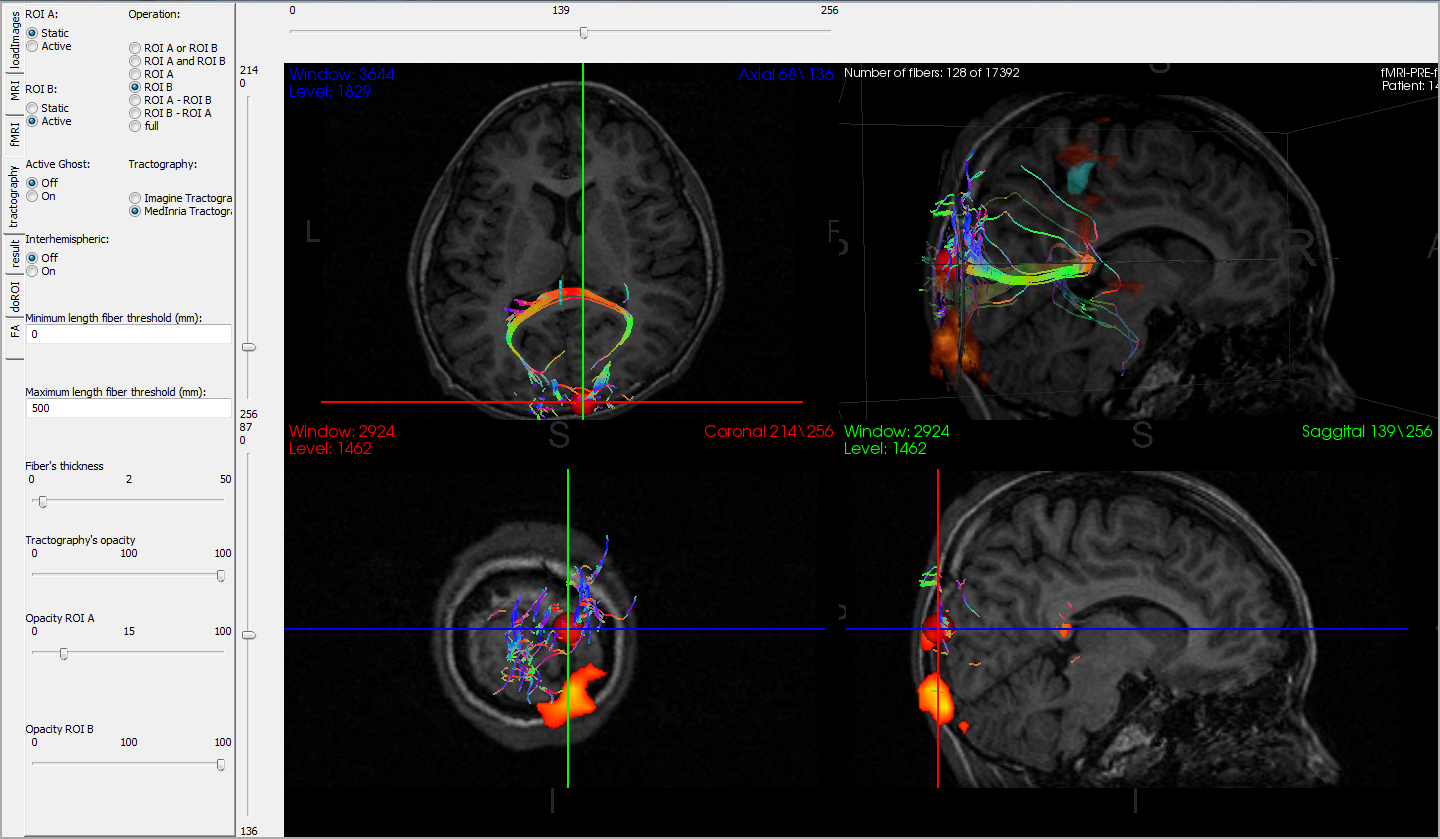
\includegraphics[width=0.9\textwidth]{historic/kab_figura1.png} 
\caption{\label{fig_kab}The main interface of KAB}
\end{figure}

The first prototype built by our group was called KAB \autocite{castro_kab:_2012}. This tool was built to analyze data from the KMC pilot study \autocite{schneider_cerebral_2012}. This software integrated data from Diffusion MRI, Functional MRI and structural MRI. The main interface of the tool is shown in figure \ref{fig_kab}. Data was pre-processed using FSL \autocite{jenkinson_fsl_2012} for skull removal and FMRI modeling, and Medinria \autocite{toussaint_medinria:_2007} for diffusion data. Registration between diffusion and structural spaces was done on-line using the tool itself. The most important features of the software were:

\begin{itemize}
\item Visualizing structural MRI, fMRI and tractography on the same space
\item Selection of bundles in a full tractography
\begin{itemize}
\item Using two spherical regions of interests located manually
\item Using conical regions of interests, representing the spread of TMS magnetic pulses
\item Using areas where fMRI statistics were above a threshold
\item Using hand-drawn regions
\end{itemize}
\item Generating statistics from selected bundles
\item Automatic generation of reports
\end{itemize}

Integrating information from different sources was the major contribution of the tool. Traditionally each type of data was analyzed on its own, using dedicated tools, and integrating information in this way was beyond brain experts. This tool was implemented based on the BBTK framework \autocite{hoyos_creatools:_2012} developed by Creatis. 

Specialists appreciated the ability to integrate several kinds of data and ask questions that involved relationships between them. During the development of the application specialists started asking questions about symmetries in the brain, and therefore the option of reflecting a ROI to the other hemisphere was added. Specialists also expressed the need of linking the coordinate system of the tool to a known atlas.

While this tool made evident the interest in integrated analysis of data, it also had some limitations.
\begin{itemize}
\item It required too much manual work, often repeating tasks
\item It had too many features in a single application, which made it complex
\item Manual registration was very error prone
\item It didn't integrate non-image data.
\end{itemize}
Based on these we proposed a new set of prototypes.

\subsection{First prototypes}

%-- titanic

For the first round of prototypes after KAB, we focused on creating tools with a limited set of features, which could run faster and be easier to learn. We stayed with the BBTK framework as it provided us a fast way to iterate. At this stage our main objectives were solving the technical problems we identified in KAB. Specifically
\begin{itemize}
\item Perform registration automatically
\item Integrate non-image data
\item Increase computational performance
\end{itemize}

\begin{figure}
\centering
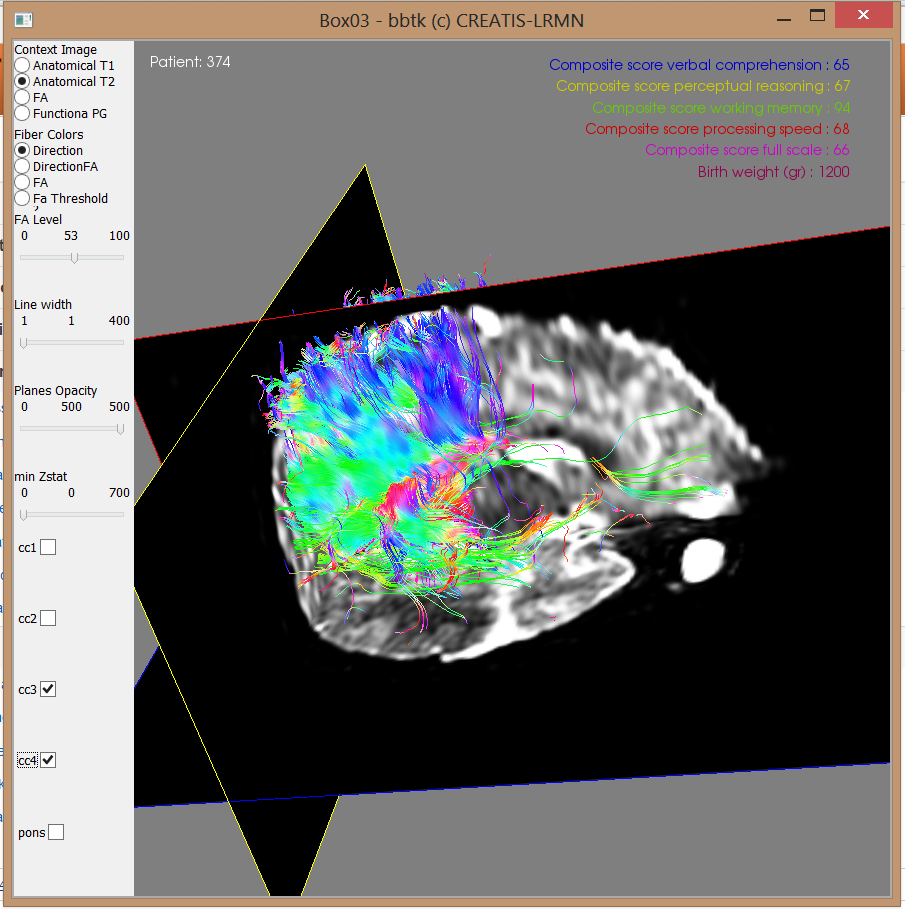
\includegraphics[width=0.9\textwidth]{historic/Titanic_B.png} 
\caption{\label{fig_titanic}Prototype integrating tabular and image data}
\end{figure}

Most of the prototypes created at this stage were only used internally to test different algorithms and techniques. Figure \ref{fig_titanic} shows the final prototype of this series. Its main features are
\begin{itemize}
\item Display values of clinical variables together with the image
\item Explicit identification of the current subject
\item Simple interface
\item Selection of different image modalities
\item Selection of different coloring schemes for bundles
\item Direct selection of the most important fiber groups
\item Control on most important visualization parameters
\end{itemize}

\begin{figure}
\centering
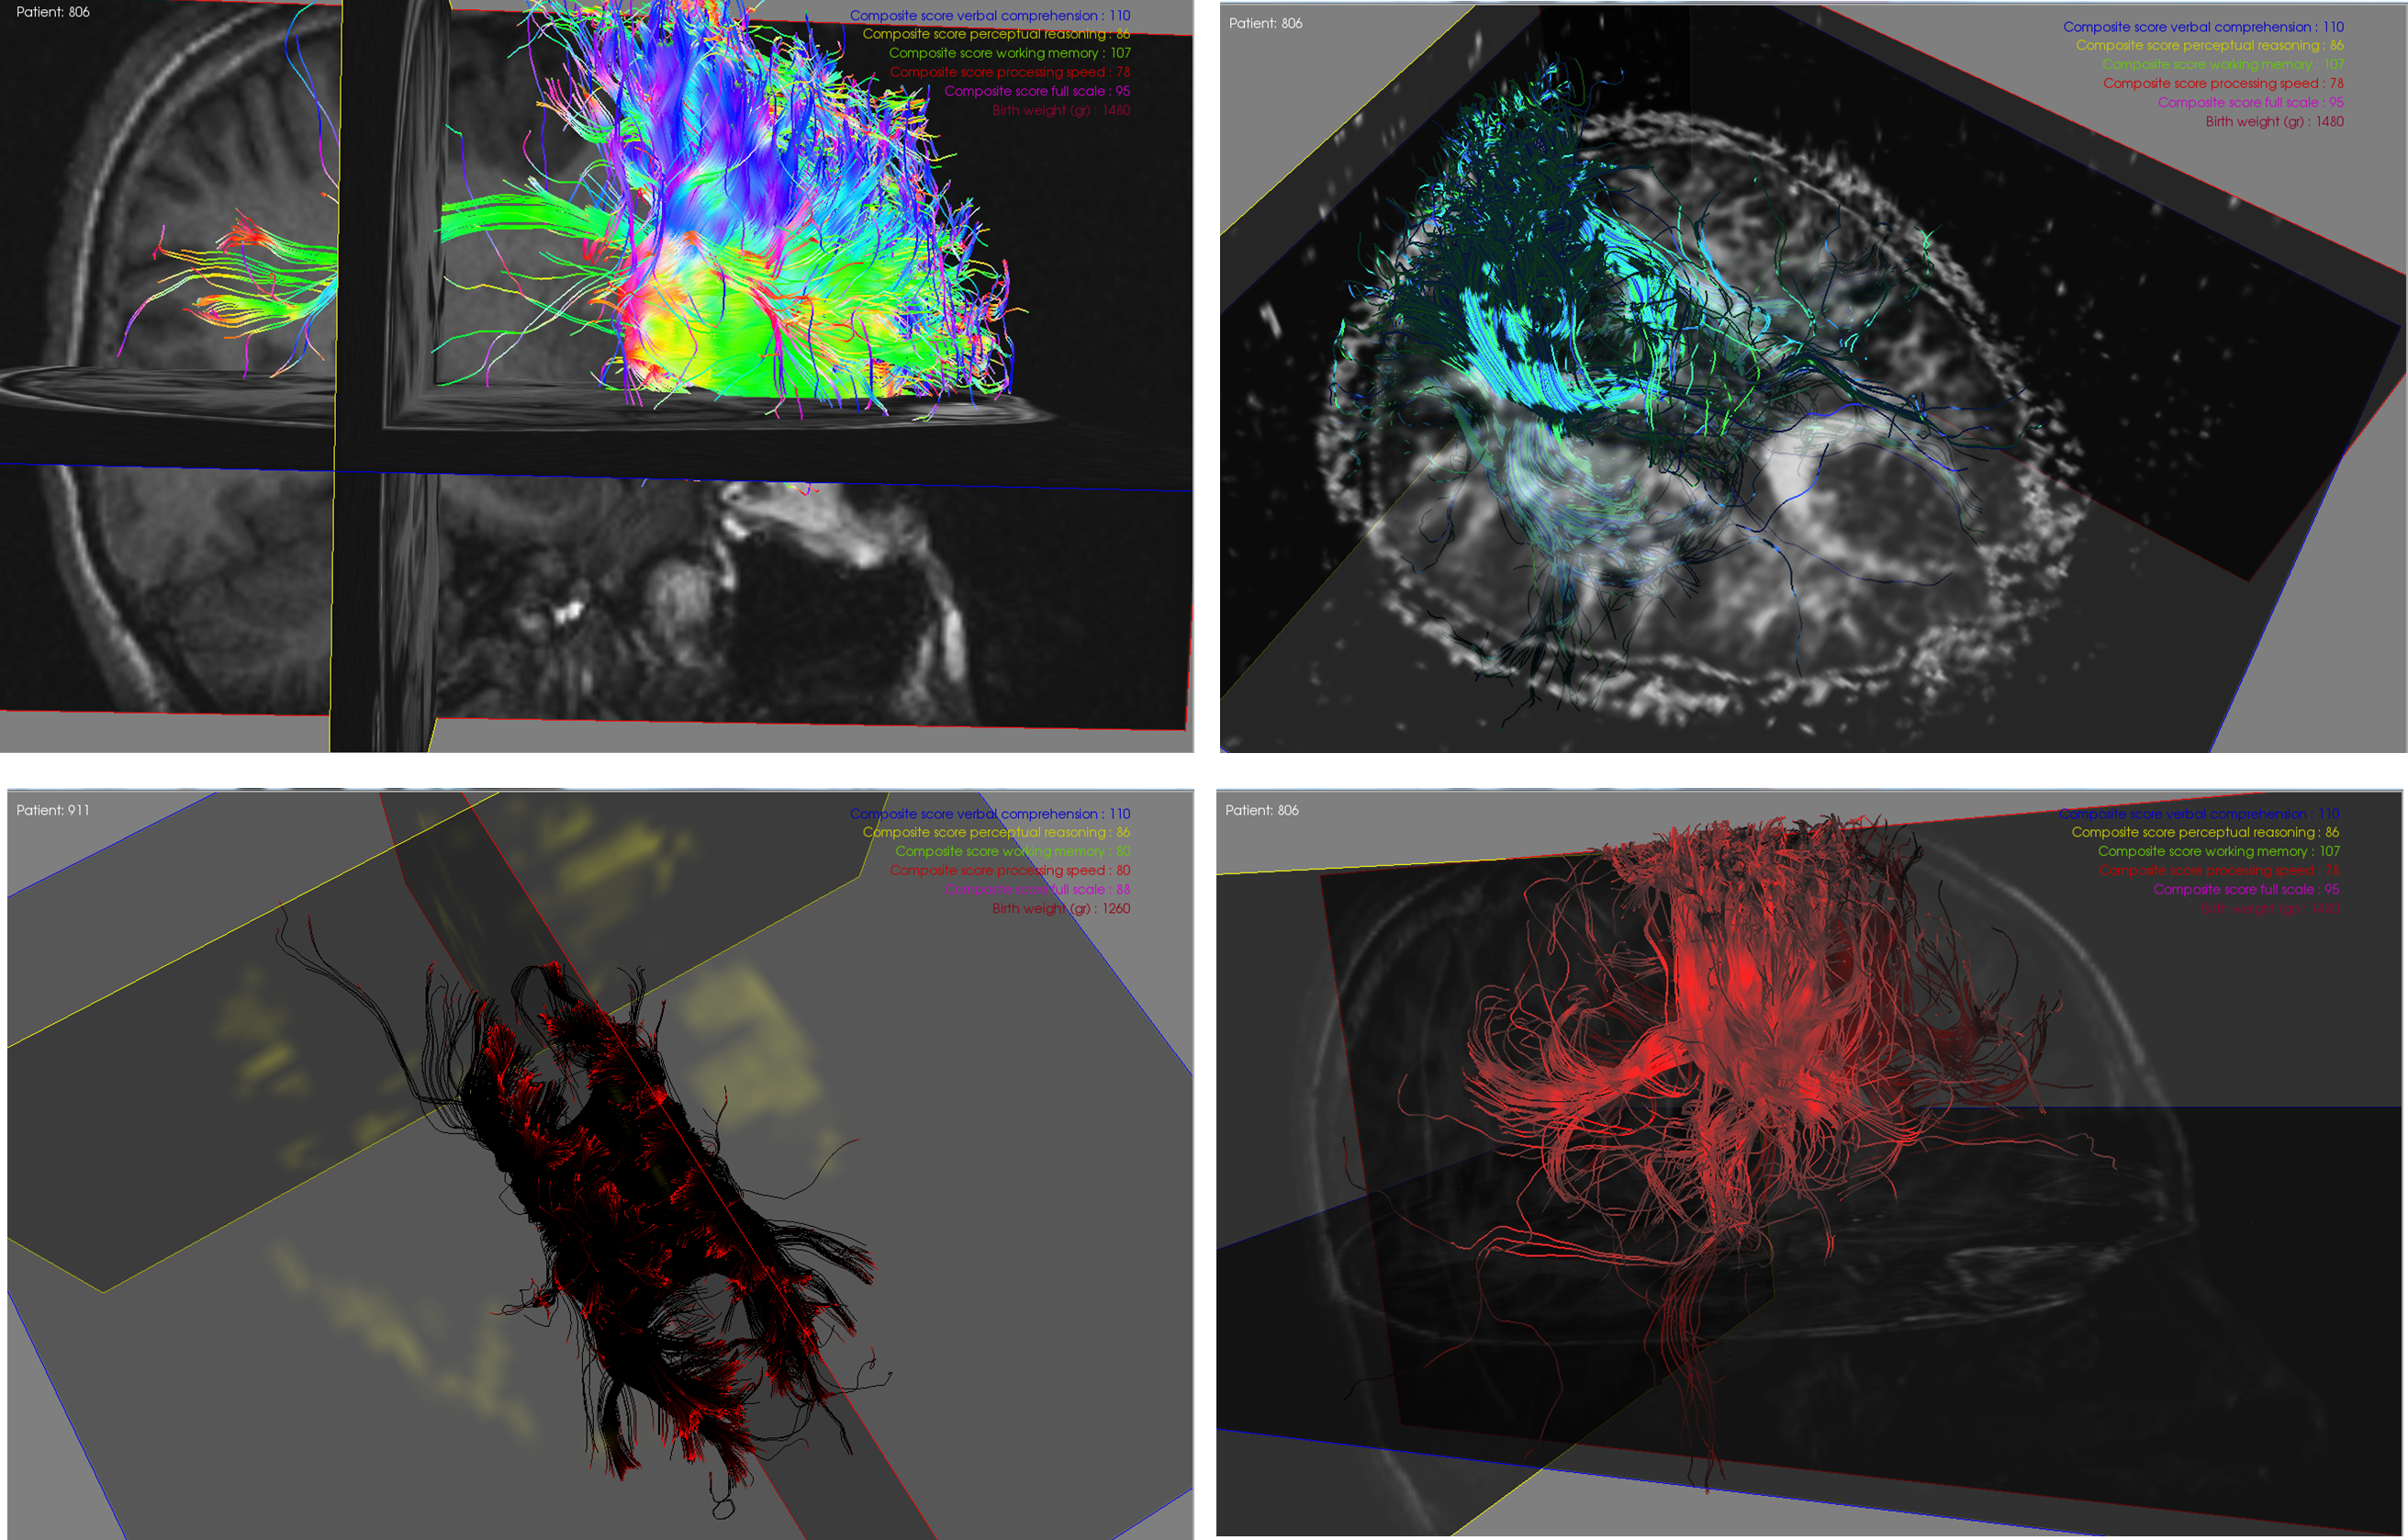
\includegraphics[width=0.9\textwidth]{historic/Titanic.png} 
\caption{\label{fig_titanic_2}The prototype could be configured to show several images and to color fibers in different ways.}
\end{figure}

Figure \ref{fig_titanic_2} shows several of the views that could be accomplished with this tool.
The tool was simple to use as there were few controls and all of them were visible. Notice this application was tailored towards the specific project. At the time the research team was specially interested in corpus callosum and motor fibers. This application allowed researchers to quickly answer specific questions relating fiber bundles to clinical variables. Also now researchers from all specialists could look at tractography and a different MRI images painlessly, where before they had to rely on large, hard to use applications. Data was organized in drive in a well defined structure. When the application launches the user only needed to select the main structural image, and the rest of the necessary files were located trough their relative paths. There was no need for end user to even know about the existence of transformation matrices or other files. This simplified a lot the process of simply looking at spatial data in context, and allowed experts to do this in a convenient way. Having a more direct access to spatial data allowed experts from different specialties to look at them on their own time, and therefore come up with new ideas for analyzes. They were also using the tool to communicate ideas to other brain experts and also to us. We now had a better way of communicating with experts, and therefore we could get a better understanding of their needs. This tool showed us the potential of integrating spatial data with clinical data, but some limitations were made evident in our work with experts
\begin{itemize}
\item It was not possible to change subject during an analysis
\item It was not easy to select different variables
\item It was not possible to use different sets of tracks
\item It is cumbersome to compare different subjects
\end{itemize}

Analyzing groups of subjects and comparing subjects became the priority for the next round.

\subsection{Braviz, First Version}

%- Braviz/tk
%-- sample applications

For the next cycle we dropped the BBTK platform as we found out it was limiting too much our design space. The platform enforced an execution model that kept everything updated. This was great for small applications, that were meant to run for just a couple of minutes. However for large applications that could run for hours we required more control of when the different modules would execute. BBTK relied on VTK for all visualization tasks, and therefor we decided to start developing directly on VTK. However it was still very important to us to have quick development cycles, and we were willing to sacrifice some performance to get it, therefore we switched our main developing language to python. In the following we will describe some of the applications developed at this stage. 

We were exploring how to bring into the applications of more sophisticated processing tools. FreeSurfer specially grabbed our attention as it provided information from an ATLAS, and provided a way to identify the different regions of the brain using common names. This was very important to experts as it allowed them to compare their finding to those of other groups, and those in the literature. Figure \ref{fig_surf_1} shows one of the prototypes which allowed experts to visualize FreeSurfer surface parcellations. This application has a 3D viewer on the right side and a control panel on the left side. The bottom part of this panel lets the user select the different FreeSurfer surfaces and scalars, while the top of the panel lets him show a subject. Notice that it is now possible to change the subject in the middle of a session, and by doing so, it is also easier to compare the same view for multiple subjects. This was one of the main goals at this stage. 

\begin{figure}
\centering
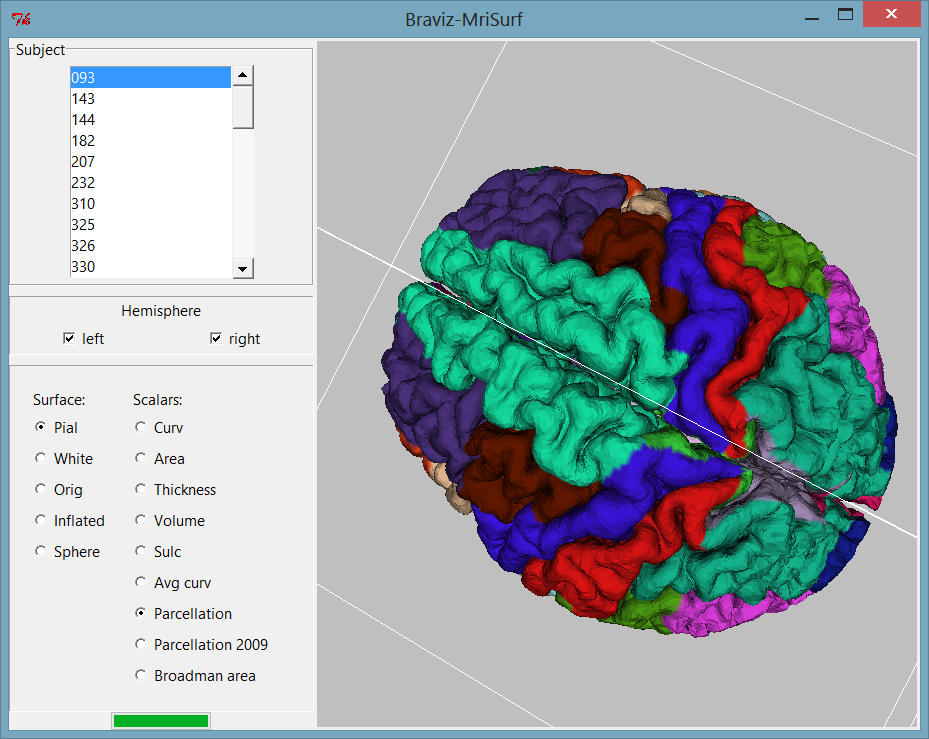
\includegraphics[width=0.9\textwidth]{historic/surf1.png} 
\caption{\label{fig_surf_1}A freesurfer surface inside Braviz}
\end{figure}

The FreeSurfer segmentations also provided us a repeatable way of selecting fibers across all subjects. Figure \ref{fig_cc_ctx_1} shows an application designed for this task. In the control panel we now have a list of structures where the user can select one or several. In the middle of the panel is a combo-box which provides the options "\emph{or}" or "\emph{and}". This selection will change the way in which multiple selections are interpreted, in the case of \emph{or}, fibers that go trough any of the structures will be selected, while in the case of \emph{and} only fibers that go trough all of them will be selected. Notice there is another combo-box labeled "\emph{coordinates}", this box provides the options "\emph{world}", "\emph{talairach}" and "\emph{dartel}". In "\emph{world}" objects on the 3D view are represented based on the coordinates of the anatomical image, in "\emph{talairach}" mode the coordinates change to the standard Talairach space and, in "\emph{dartel}" mode, objects are registered to sample template using a non-linear registration. By moving to a standard space comparing two different subjects is easier, as some of the differences will be absorbed by the transformation. This will enhance some types of differences but will hide some others; the most appropriate coordinate system will depend on what types of differences are currently of interest for the end user. In this application several other FreeSurfer structures could be added to the scene in order to provide context. Figure \ref{fig_fibers_ctx} shows another view of this application. By hovering the cursor on top of a bundle the user could get some information about them. It was also possible to measure distances in the 3D space in order to make numeric comparisons across subjects.

\begin{figure}
\centering
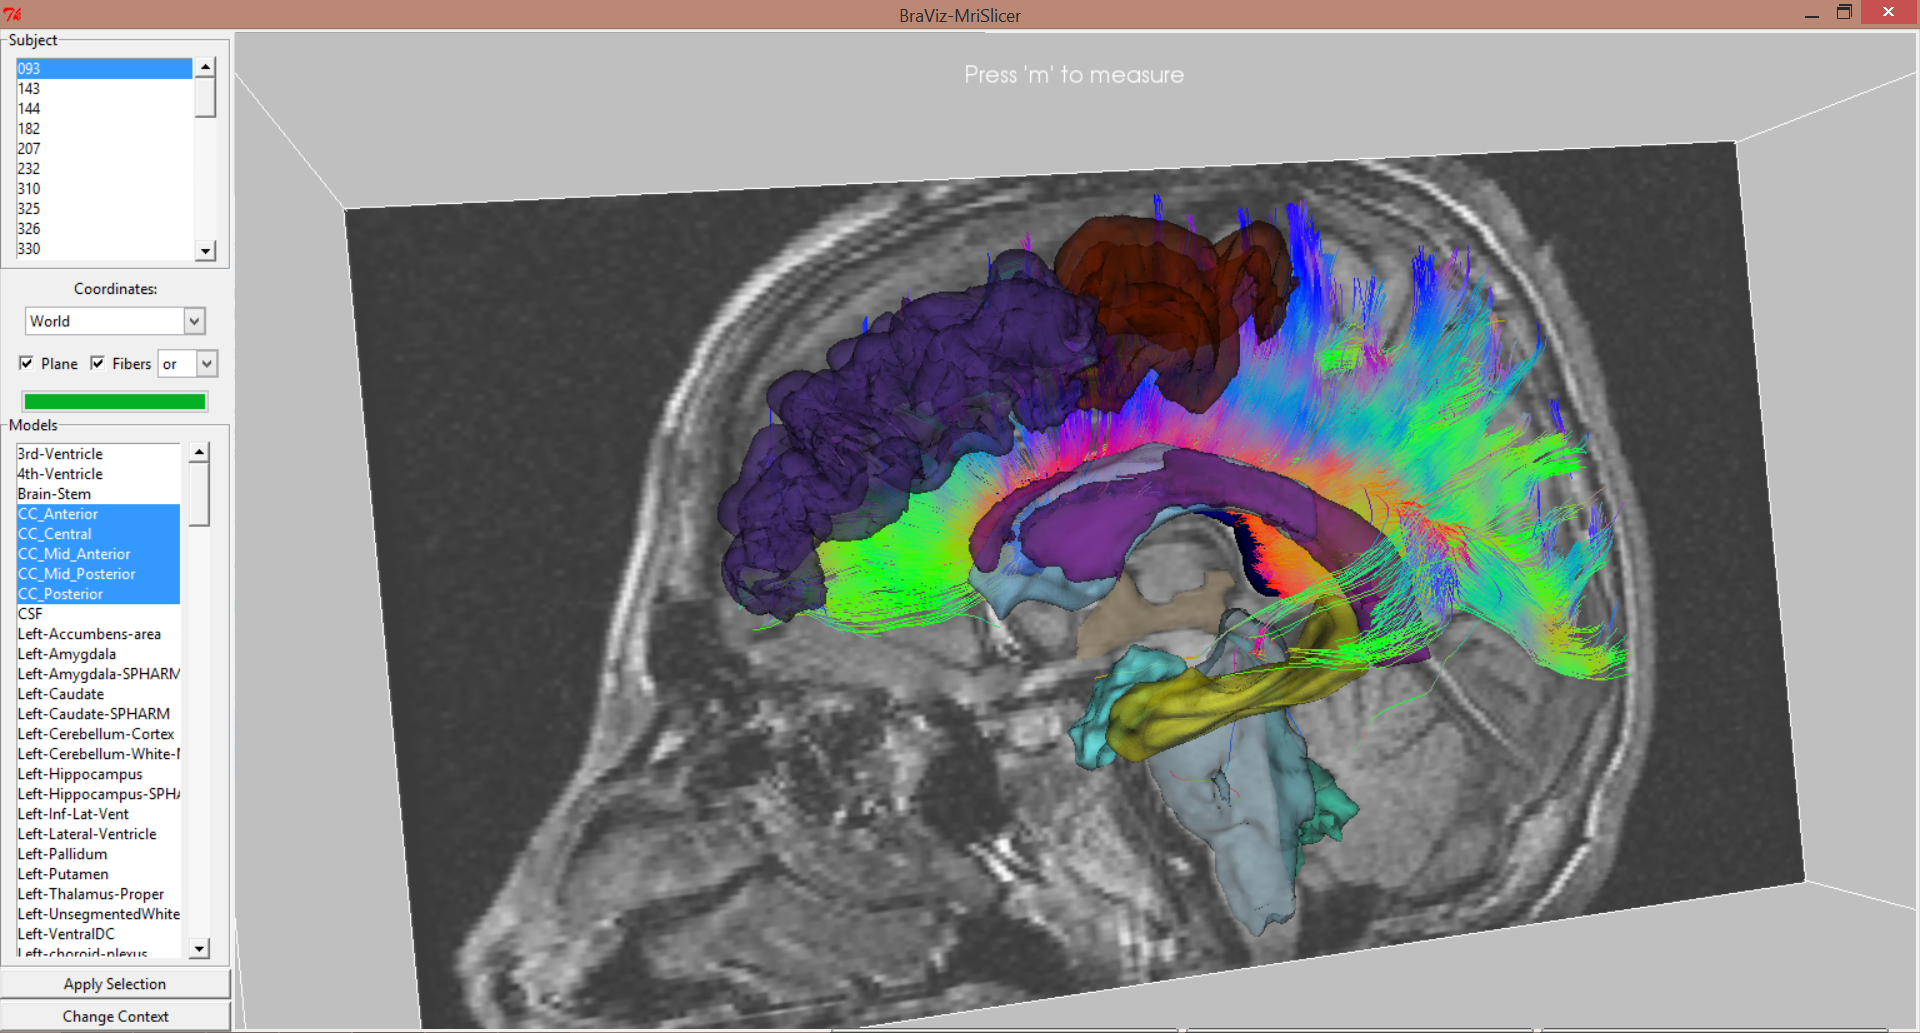
\includegraphics[width=0.9\textwidth]{historic/cc_in_context.png} 
\caption{\label{fig_cc_ctx_1}Fibers of the corpus callosum with segmentation and anatomical image as context}
\end{figure}

\begin{figure}
\centering
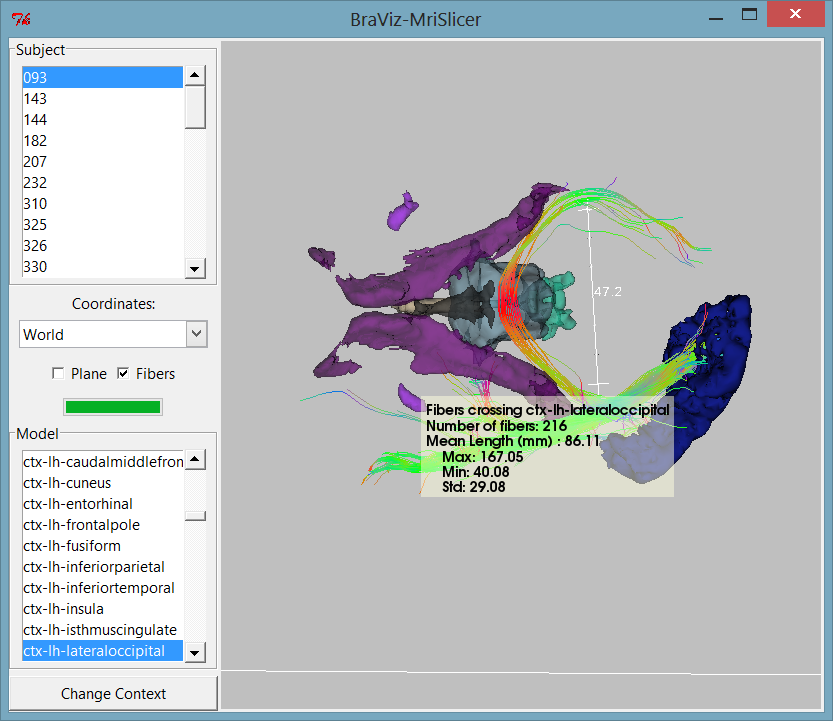
\includegraphics[width=0.9\textwidth]{historic/fibers_in_context.png} 
\caption{\label{fig_fibers_ctx}Fibers could be selected using freesurfer segmentation. Vtk widgets could be used to make measurements.
Additionally statistics of each bundle were also available.}
\end{figure}

An application for viewing two subjects at the same time and comparing them was also created. Its interface can be seen on figure \ref{fig_compare_1}. In this application it was possible to show the same selection of images, fibers and structures for two different subjects. The screen could be split vertically, horizontally or both subjects could be shown on the same space but using different colors and possibly adding a small offset. In the case of split screen the camera in both views was coordinated, and there was the possibility to add a plane that would be replicated in both views to use as context.

\begin{figure}
\centering
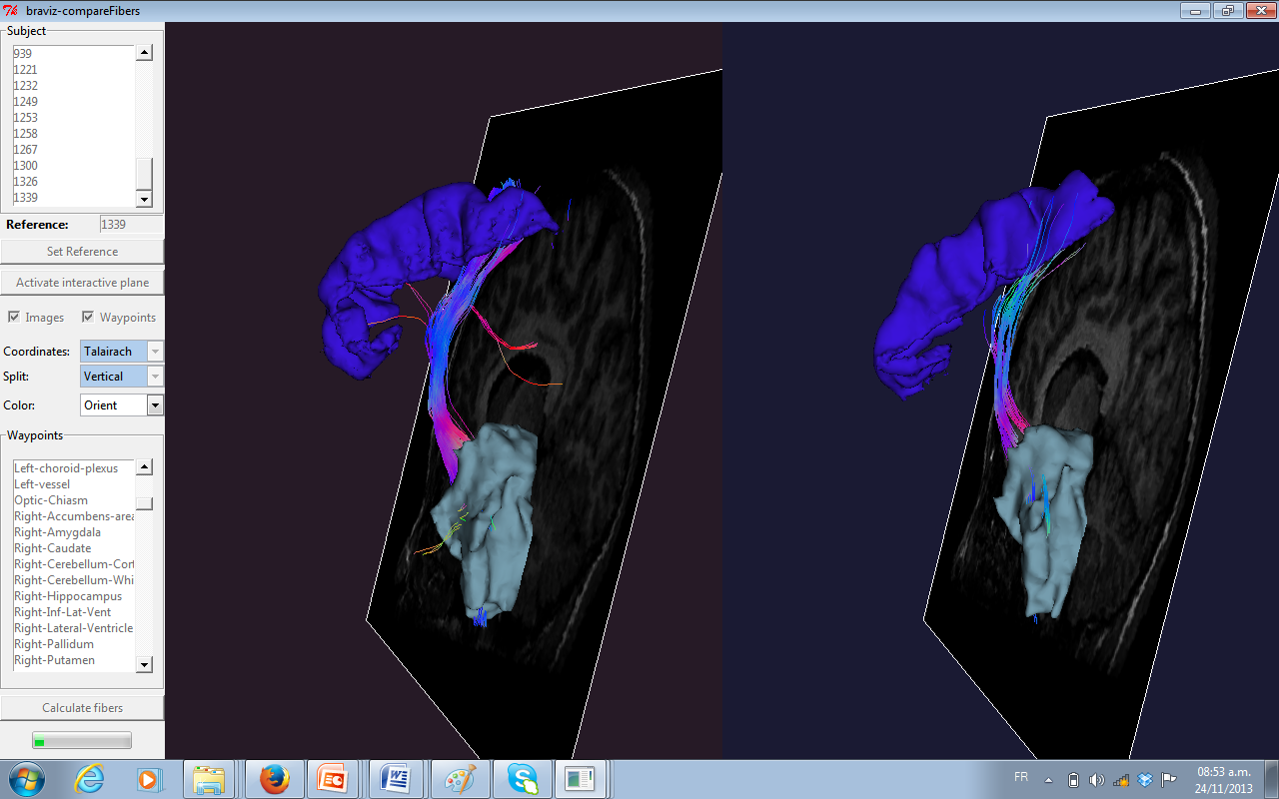
\includegraphics[width=0.9\textwidth]{historic/compare.png} 
\caption{\label{fig_compare_1}Comparing the motor tract of two subjects}
\end{figure}

At this point the interest in fMRI was increasing, but some of the researchers who were not expert on this technique were having problems interpreting this data correctly. Figure \ref{fig_fmri_1} shows an application created to make the nature of fMRI explicit. The application shows the T-score image in the 3D view, but also shows the corresponding time signal at each voxel, together with the experiment design. In this way users could better understand that a higher score meant a larger relationship between the BOLD signal an the paradigm. 

\begin{figure}
\centering
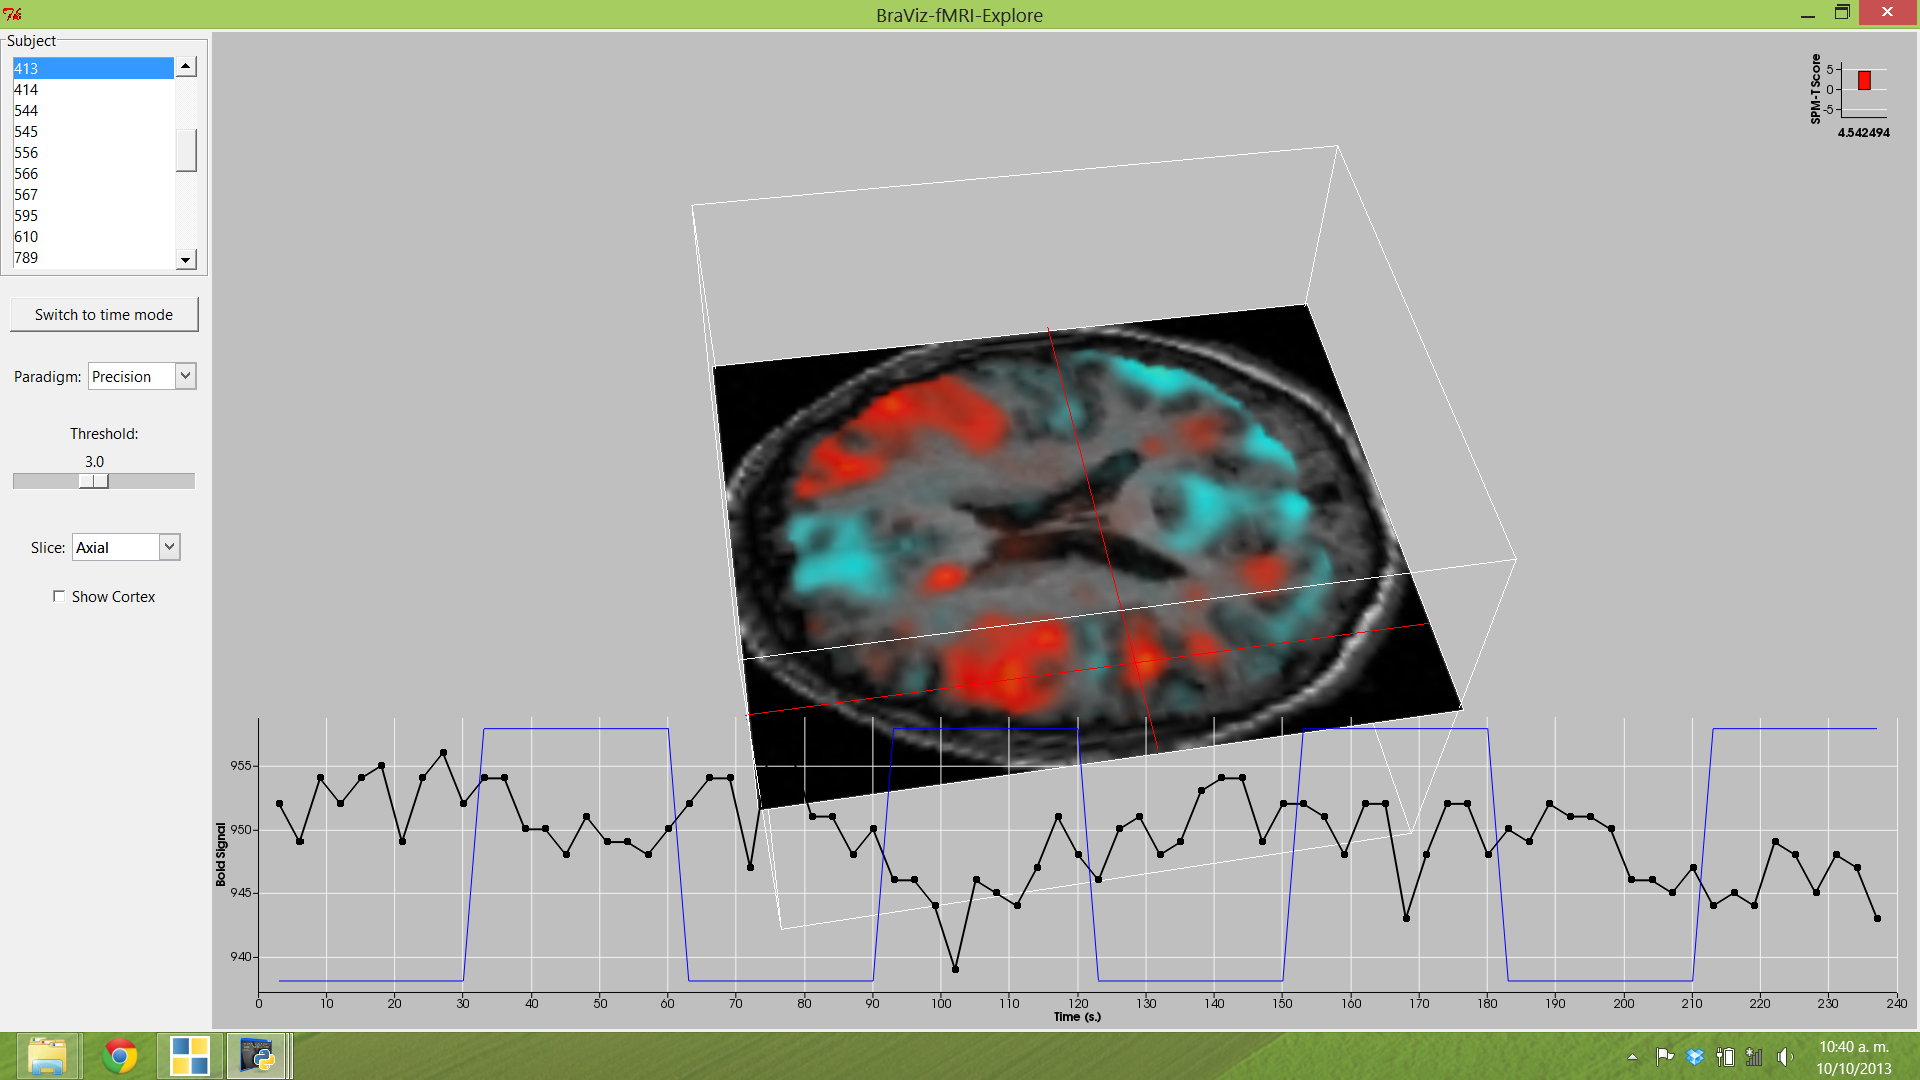
\includegraphics[width=0.9\textwidth]{historic/rejean2.png} 
\caption{\label{fig_fmri_1}This prototypes make the time dimension of fMRI explicit, therefore helping non-experts understand its meaning and make better interpretations}
\end{figure}

We wanted to let researchers search for patterns between clinical variables and structures. One proposal in this direction can be seen in figure \ref{fig_grid}, this application shows the corpus callosums of all subjects in the study organized in a grid. From left to right the structures are organized according to a clinical variable, while the color of the structures reflect the value of another clinical variable. The variables used for these purposes could be selected from the panel on the left. At the bottom right of the viewer was a small scatter plot showing the relationships between the two variables. This plot was linked to the grid view, so selecting a point in the plot would highlight the corresponding structure and vice versa. Another important feature was that an individual structure could be rotated in 3d space, and the rotations would be propagate to all the structures on the grid.

\begin{figure}
\centering
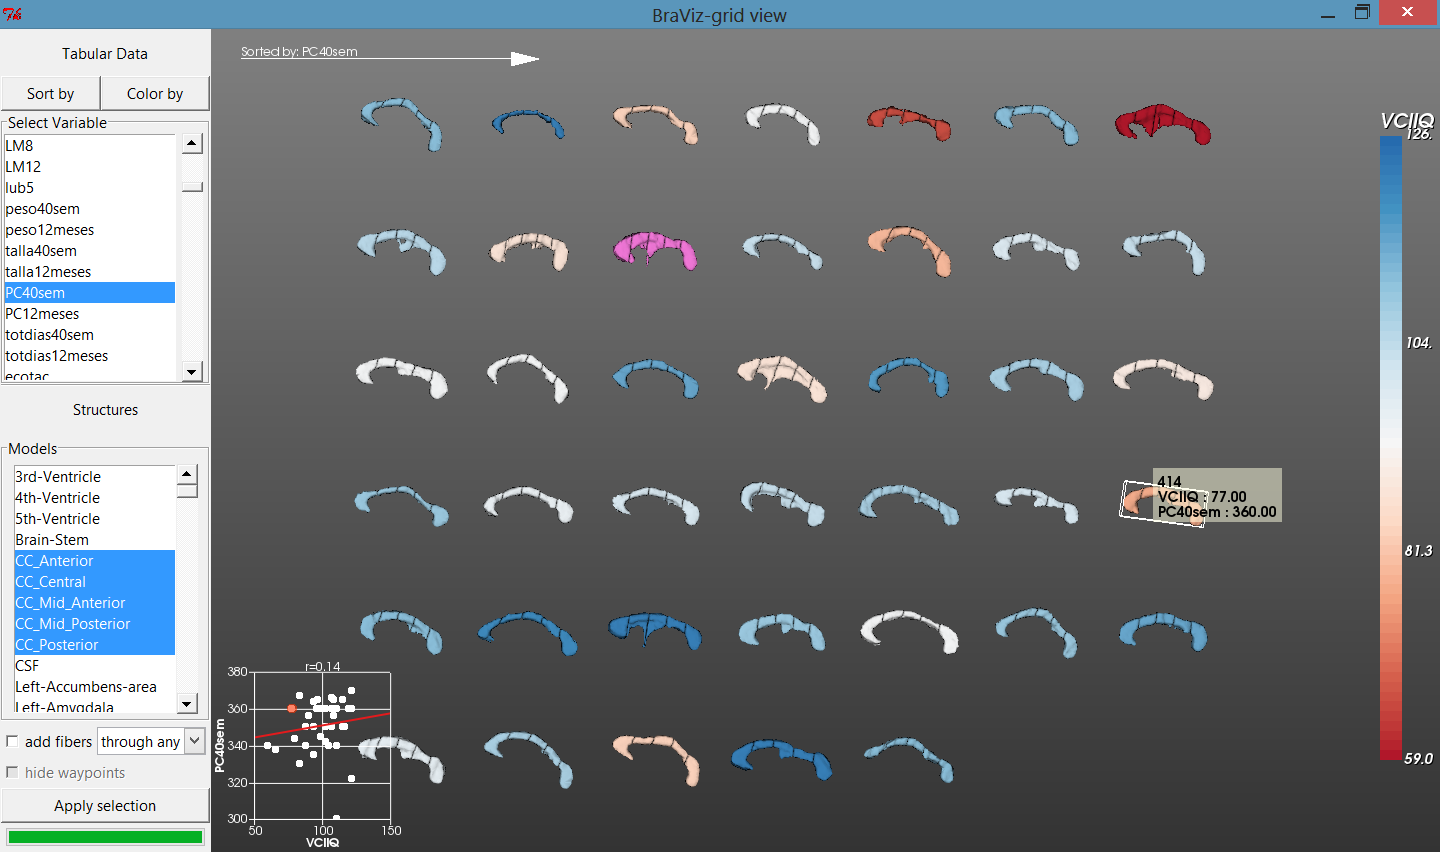
\includegraphics[width=0.9\textwidth]{historic/grid_and_scatter.png} 
\caption{\label{fig_grid}Corpus Callosums of several subjects organized on a grid and colored with respect to clinical variables.
A scatter plot of these variables is shown at the bottom left}
\end{figure}

Another proposal for showing relationships between structures and clinical variables is shown in figure \ref{fig_star_1}. In this case structures and data are separated in three groups. This grouping is done by the main categorical variable in the study (see chapter \ref{chap_kmc}). Clinical data is shown using a spider plot, where each subject is represented as a polygon and each variable is an axis. Structures are shown on the same space using alpha-blending. By mixing all the structures in this way the average shape for the group appears. Also notice variables are organized in a tree like structure on the top left, and the description of each variable appears when the user hovers on its name. This tree also showed FreeSurfer structures and allowed the user to add the volumes and areas of such structures to the star plot. As in the previous case there was an integration between the numerical variables and the structure, and clicking on one would highlight the corresponding subject on both views.

\begin{figure}
\centering
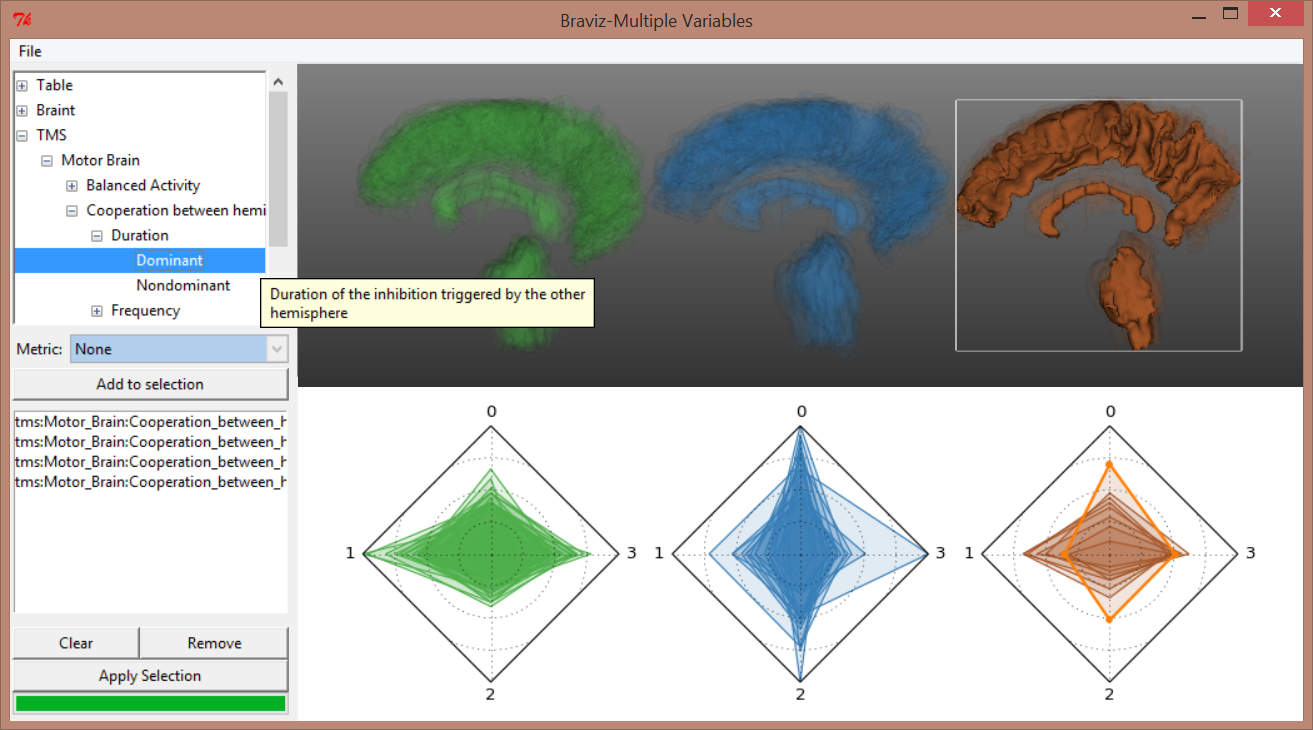
\includegraphics[width=0.9\textwidth]{historic/mini_star.png} 
\caption{\label{fig_star_1}This application allowed comparing several structures and variables between groups of subjects.}
\end{figure}

The application shown in figure \ref{fig_tms_1} was developed for a very specific task: analyzing the relationship between TMS metrics with fibers. The application shows at the left a list of tms variables organized in a tree, a selection between dominant and non-dominant hemisphere, and the option to add males or females to the sample. In this case the application would know if a given subject is right handed or left handed, and display the values for the dominant or non-dominant hemisphere. At the bottom of the screen the values for the whole sample would be shown with the current subject on the right. The picture at the top of the screen would display the motor fibers where the current metric only involved one hemisphere, and the corpus callosum (see figure \ref{fig_tms_2}) where the current metric involved both hemispheres. The user could click on a bar on the bottom display and select that subject.
It was also possible to show aggregated measures for the three groups on the bottom display as seen in figure  \ref{fig_tms_2}. By doing this the expert could quickly evaluate the relationship between the visual appearance of tractography and values of tms metrics. 

\begin{figure}
\centering
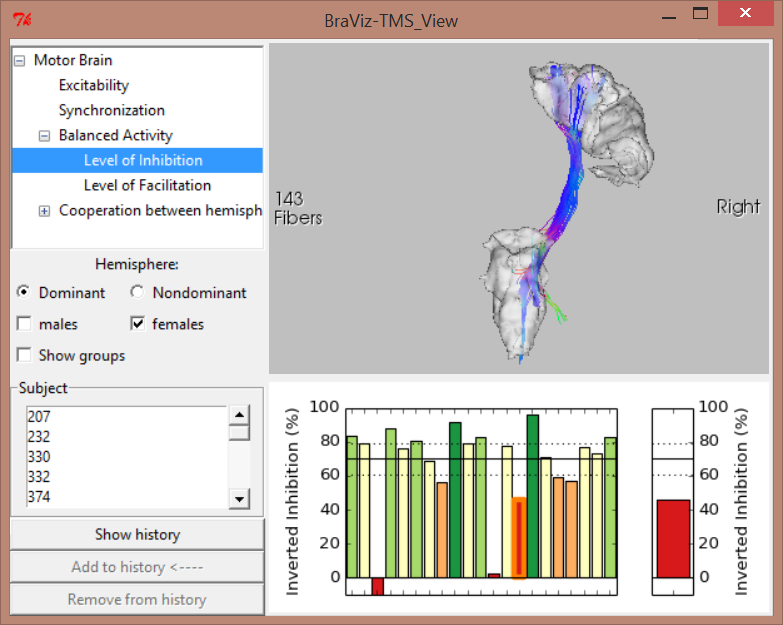
\includegraphics[width=0.9\textwidth]{historic/mini_tms.png} 
\caption{\label{fig_tms_1}An application tailored at analyzing TMS variables relationship with tractography}
\end{figure}

\begin{figure}
\centering
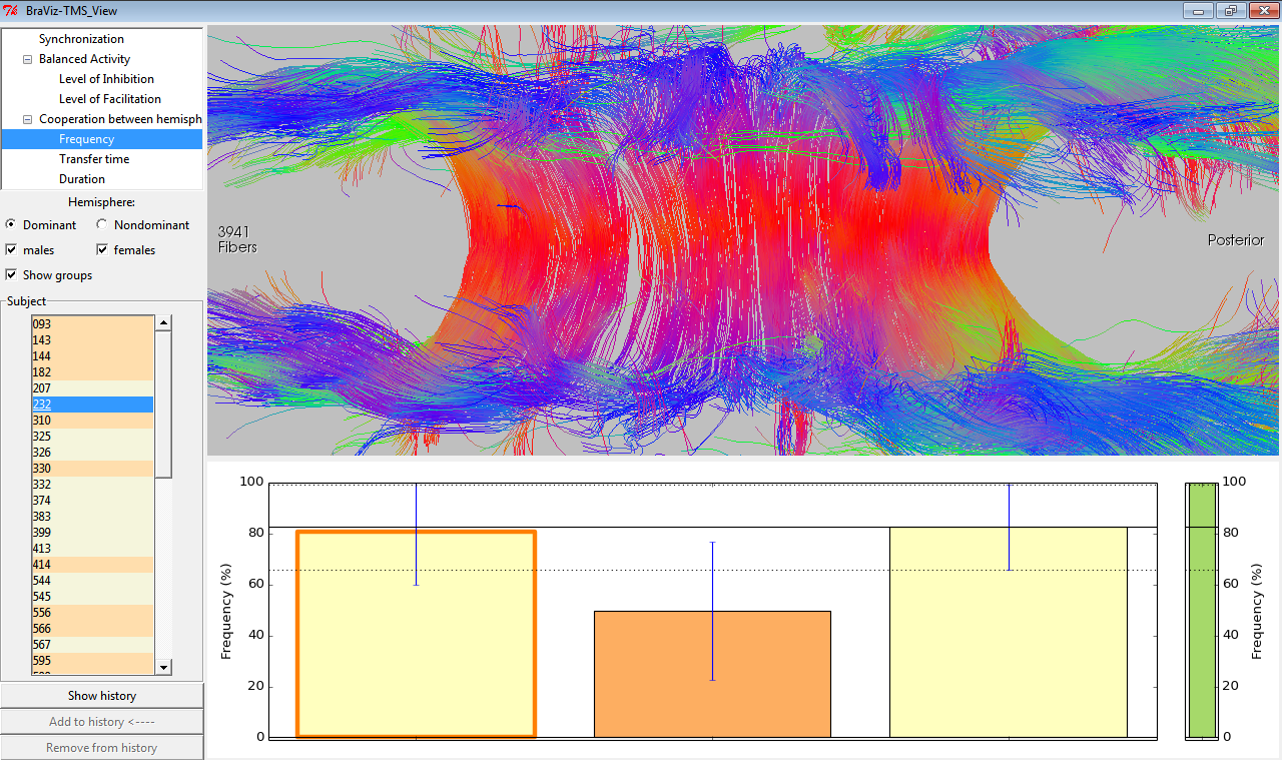
\includegraphics[width=0.9\textwidth]{historic/tms_2.png} 
\caption{\label{fig_tms_2}Another view of the TMS applications, this time showing the fibers of the corpus callosum.}
\end{figure}

Finally, we created a menu in order to group all applications and provide users with a direct access point to all of them. Before this, we had a collection of icons in a folder, but users found it complex. Trough the menu they can see a picture of each application, and therefore find the one they need without even reading.

\begin{figure}
\centering
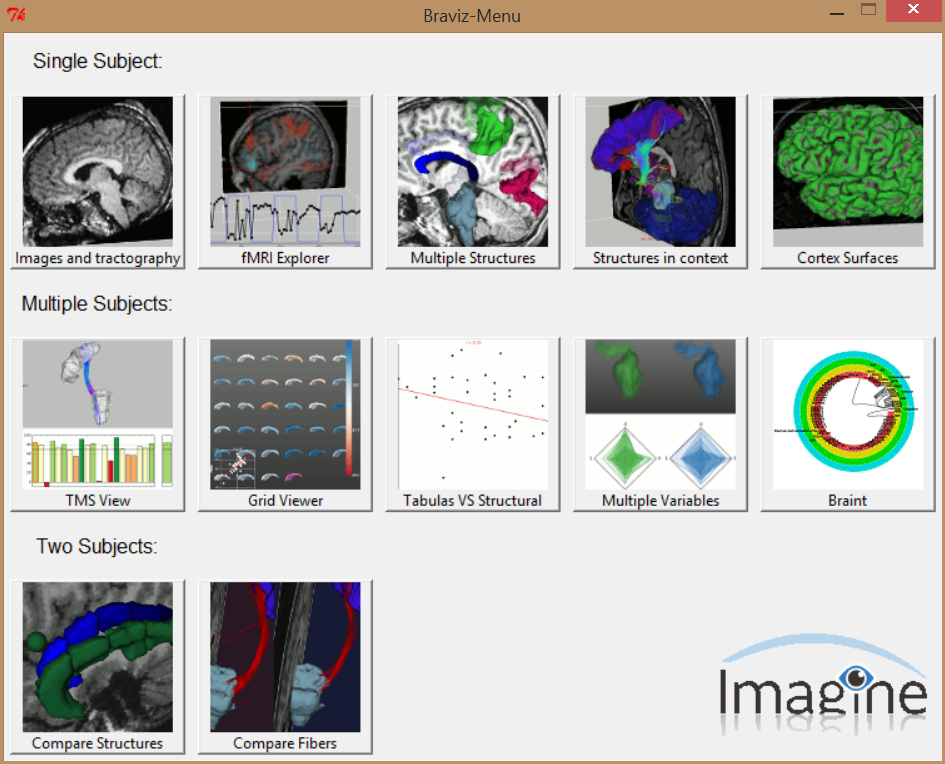
\includegraphics[width=0.9\textwidth]{historic/braviz_menu.png} 
\caption{\label{fig_menu_1}A menu was provided to give an overview of the available applications and provide simple access.}
\end{figure}

By this iteration we had more confidence in the underlying data analysis steps, and therefore were able to propose a wide array of solutions. We got closer to our goal of analyzing groups of subjects and integrating clinical variables with structural data. The features users liked the most were

\begin{itemize}
\item Seeing the same display for different subjects
\item Associating locations in the image to areas in an Atlas
\item Relating Volumes, Areas and Lengths of fibers to clinical variables
\item Quickly seeing relationships between clinical variables
\end{itemize}

As it can be seen the interest in the analysis of clinical values was increasing. In fact the favorite feature from the grid viewer in figure \ref{fig_grid} was the scatter plot at the corner. We were somehow disappointed for the lack of interest in the 3D graphs, but those were the opinions of the users. In fact they mentioned that hardly anything could be seen in the alpha blended images from figure \ref{fig_star_1}. In other views they were happy to be able to see the data, but they demanded even more for numerical measures where statistics could be applied. Therefore the main goal for the next iteration was improving the support for clinical data.

%Feedback

\subsection{Braviz, Second Version}

%- Braviz Qt
%-- sample applications

The first version of Braviz provided a robust infrastructure for displaying spatial data on multiple coordinate systems, however its ability to handle clinical variable was still limited. From the last iteration we realized that in order to efficiently use the data we needed some analytics on the variables. We also required a better infrastructure to store and manipulate this variables. Another limitation of the previous prototype was that work could not be saved or restored. Measurements derived from segmented structures or fibers were separated from clinical variables. Finally, all of the applications operated independently without any connection. This version of Braviz addresses those limitations. 

In order to store and manage clinical variables and those derived from spatial data a database was integrated in the system. This database is also used to let user store and retrieve data. Details of the database will be given on section \ref{sec_tech}. Applications were coordinated by sharing the same database, and by passing messages between them. The model described in chapter \ref{chap_model} was mature by this moment, and was the basis for this implementation. Section \ref{sec_arch} will provide a closer look at how the model is realized into this platform, but first we will take a look at some of the features of this version.

\begin{itemize}
	\item Centralized storage of variables and user data
	\item Importing and Exporting variables to/from spreadsheets
	\item Coordinated applications, can focus on the same subject on all applications
	\item New QT based user interface
	\item Create new variables based on spatial data and add them to the database
	\item Statistical processing based on R
	\item Create, use and share custom sub-samples
	\item Save and restore the state of applications
\end{itemize}

We took all of the different data viewers of the previous iteration and combined them into a single viewer, called \emph{subject overview}. This viewer can be used to show all the different kinds of data that are available on the same space. Several of the possibilities are shown on figure \ref{fig_subj_viewer_mosaic}. The main interface of this application is shown in figure \ref{fig_subj_overview_2}. Notice that below the main view now we can find the values of several values for the current subject. Another feature is that the viewer lets the user calculate scalar metrics based on the objects in the scene, and add this values to the database as a new variable.

\begin{figure}
\centering
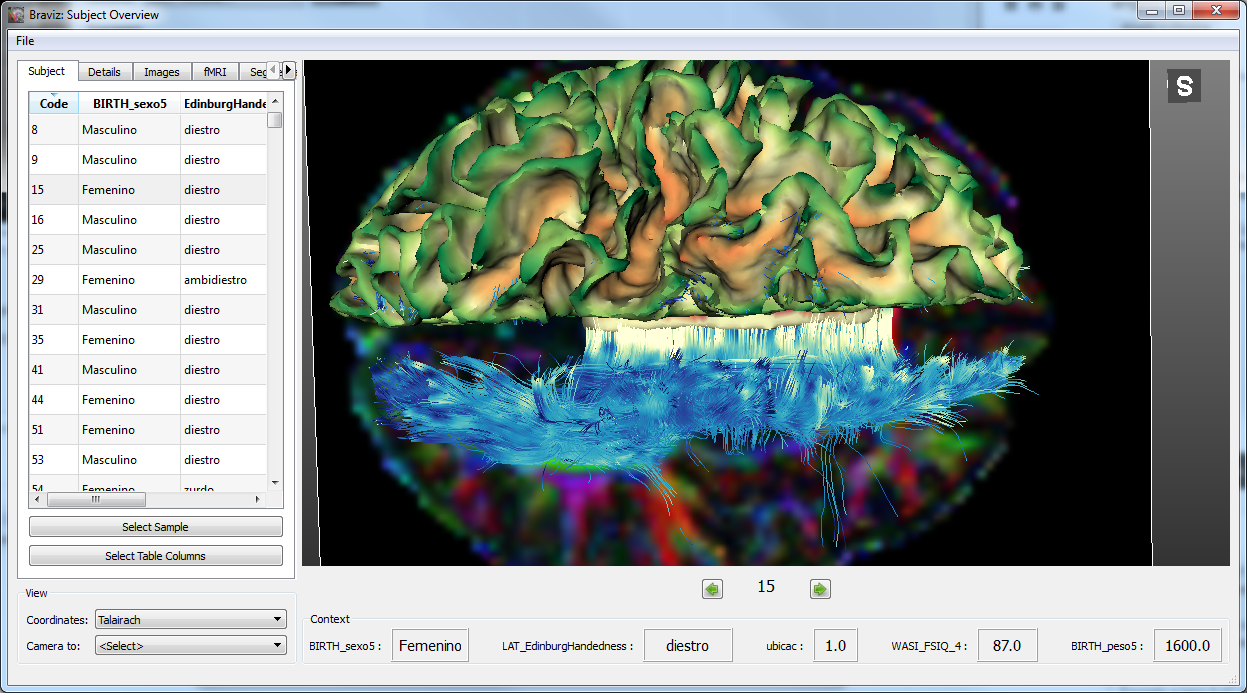
\includegraphics[width=0.9\textwidth]{braviz_qt/subj_overview_full.png} 
\caption{\label{fig_subj_overview_2}The new subject viewer integrates all of the data-types from previous version on the same application, therefore allowing all types of combinations.}
\end{figure}

\begin{figure}
\centering
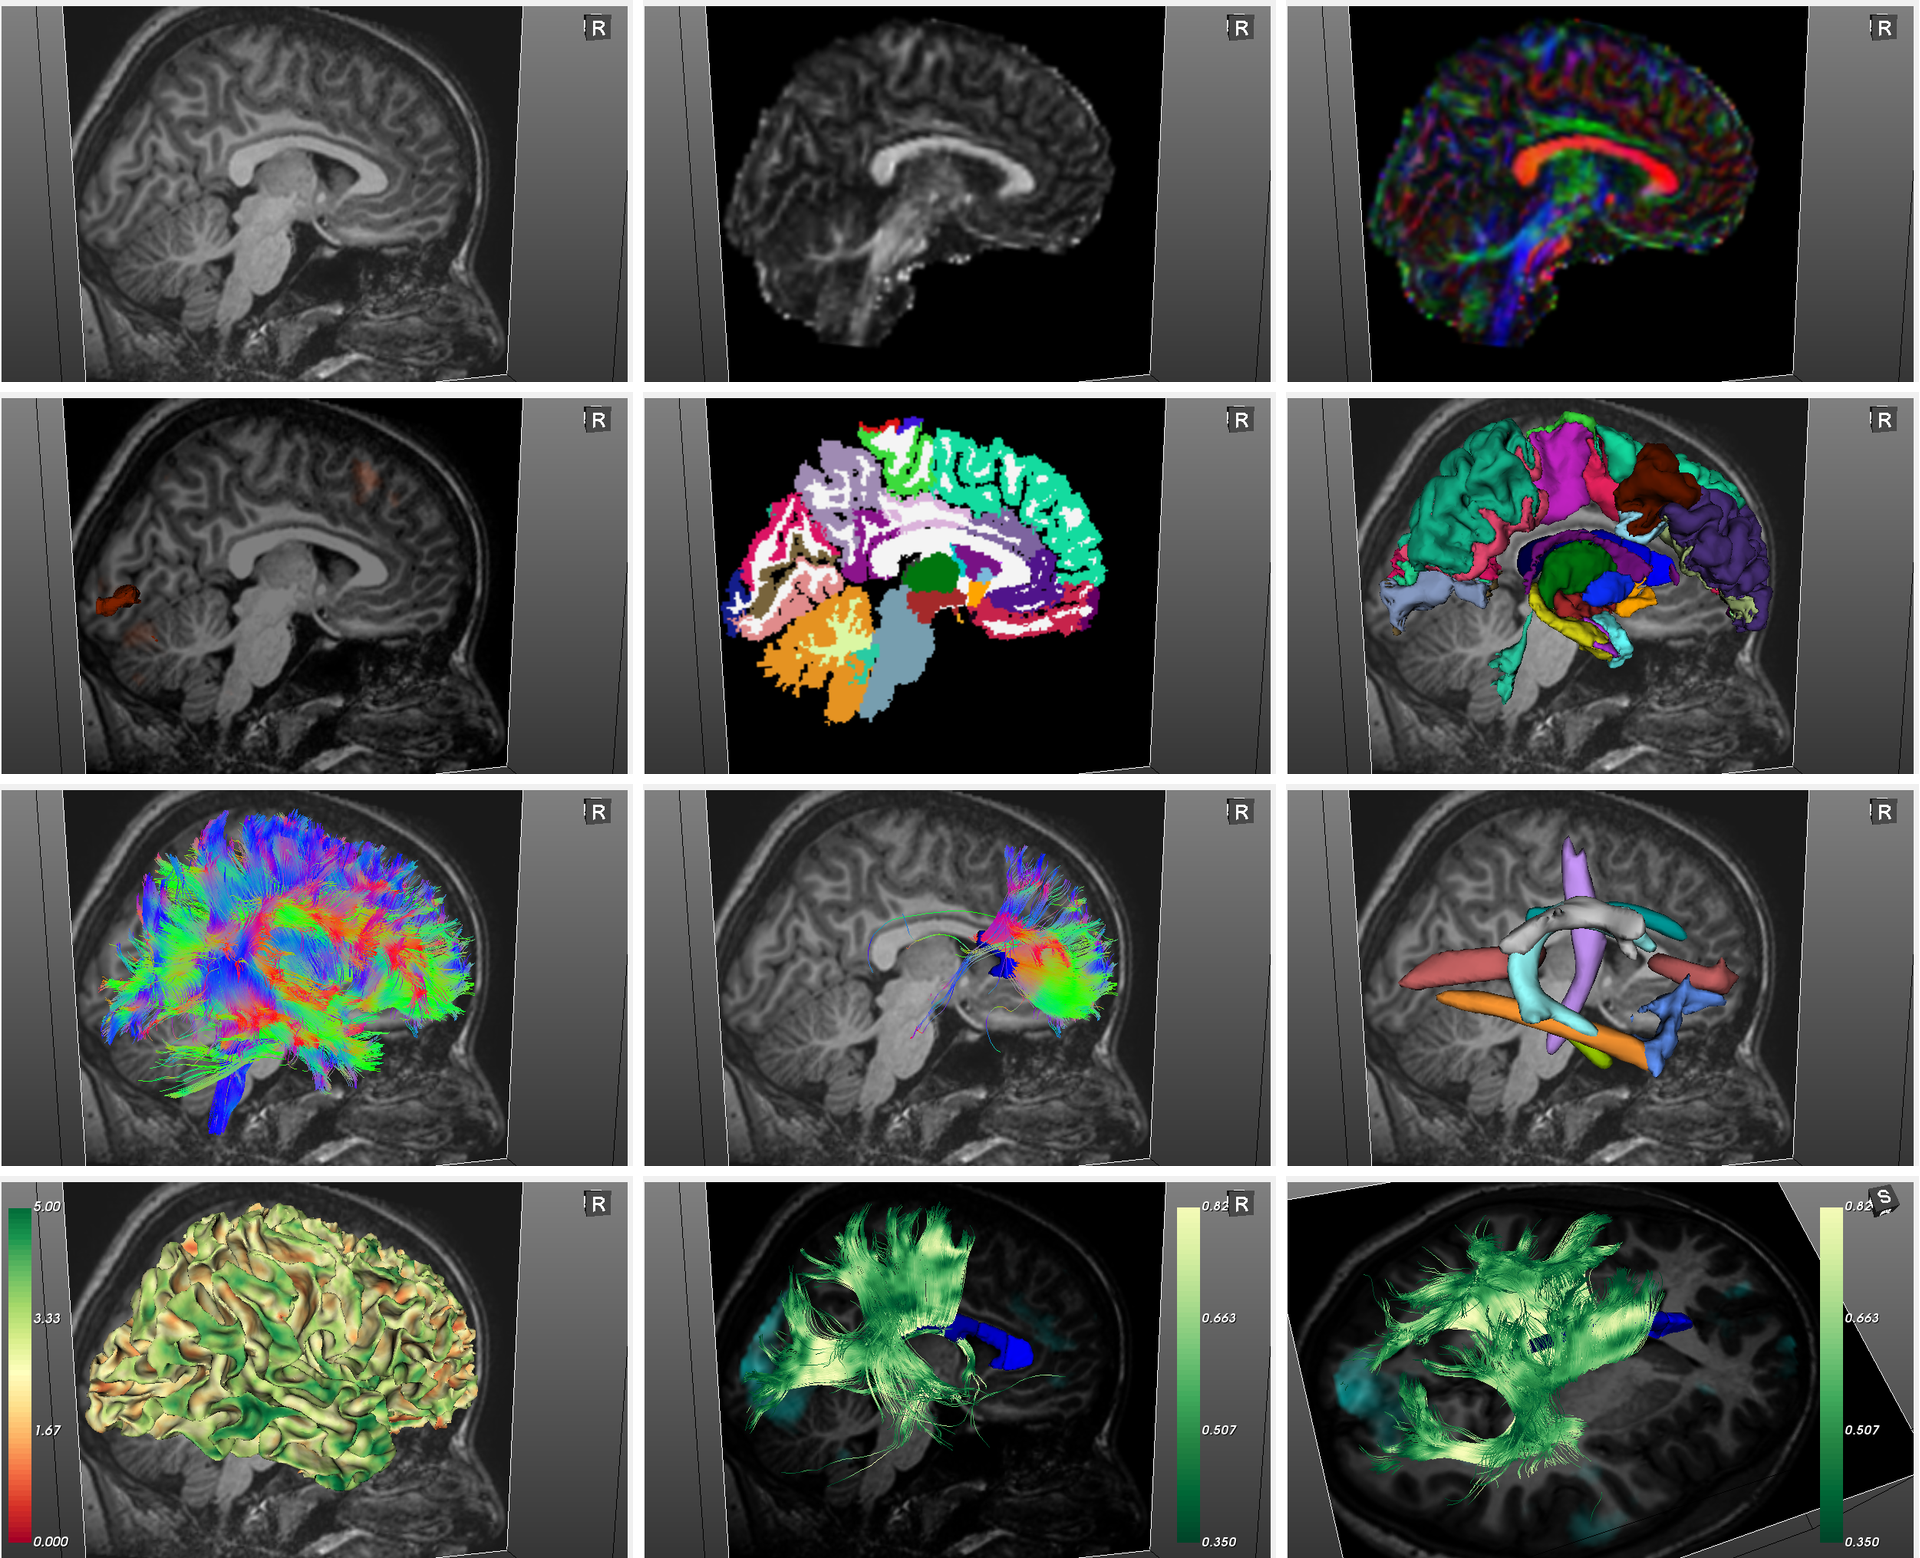
\includegraphics[width=0.9\textwidth]{braviz_qt/subj_viewer_mosaic.png} 
\caption{\label{fig_subj_viewer_mosaic}Examples of visualizations that can be achieved with the new subject viewer.}
\end{figure}

The application shown in figure \ref{fig_sample_overview_2}, called \emph{sample overview}, lets the expert look at several subjects at the same time. Subjects are arranged in rows based on a nominal variable and from left to right based on a numerical value. The values of this variables are also shown on the bar plots at the right. Each bar is linked to one 3d viewer, and by selecting a subject on one of the view it will be highlighted on the other one. As before it is possible to manipulate the camera on one viewer and copy it to the rest. Notice that we abandoned the idea of alpha blending in favor of multiple views that we expect will be easier to interpret. If more details from a single subject are required, the user can right click on the small picture, and from the context menu select \emph{show in other viewers} or \emph{show in new viewer}. The first option will highlight the subject on all opened viewers, while the second one will launch a new subject overview subject configured in the same way as the small viewer.

\begin{figure}
\centering
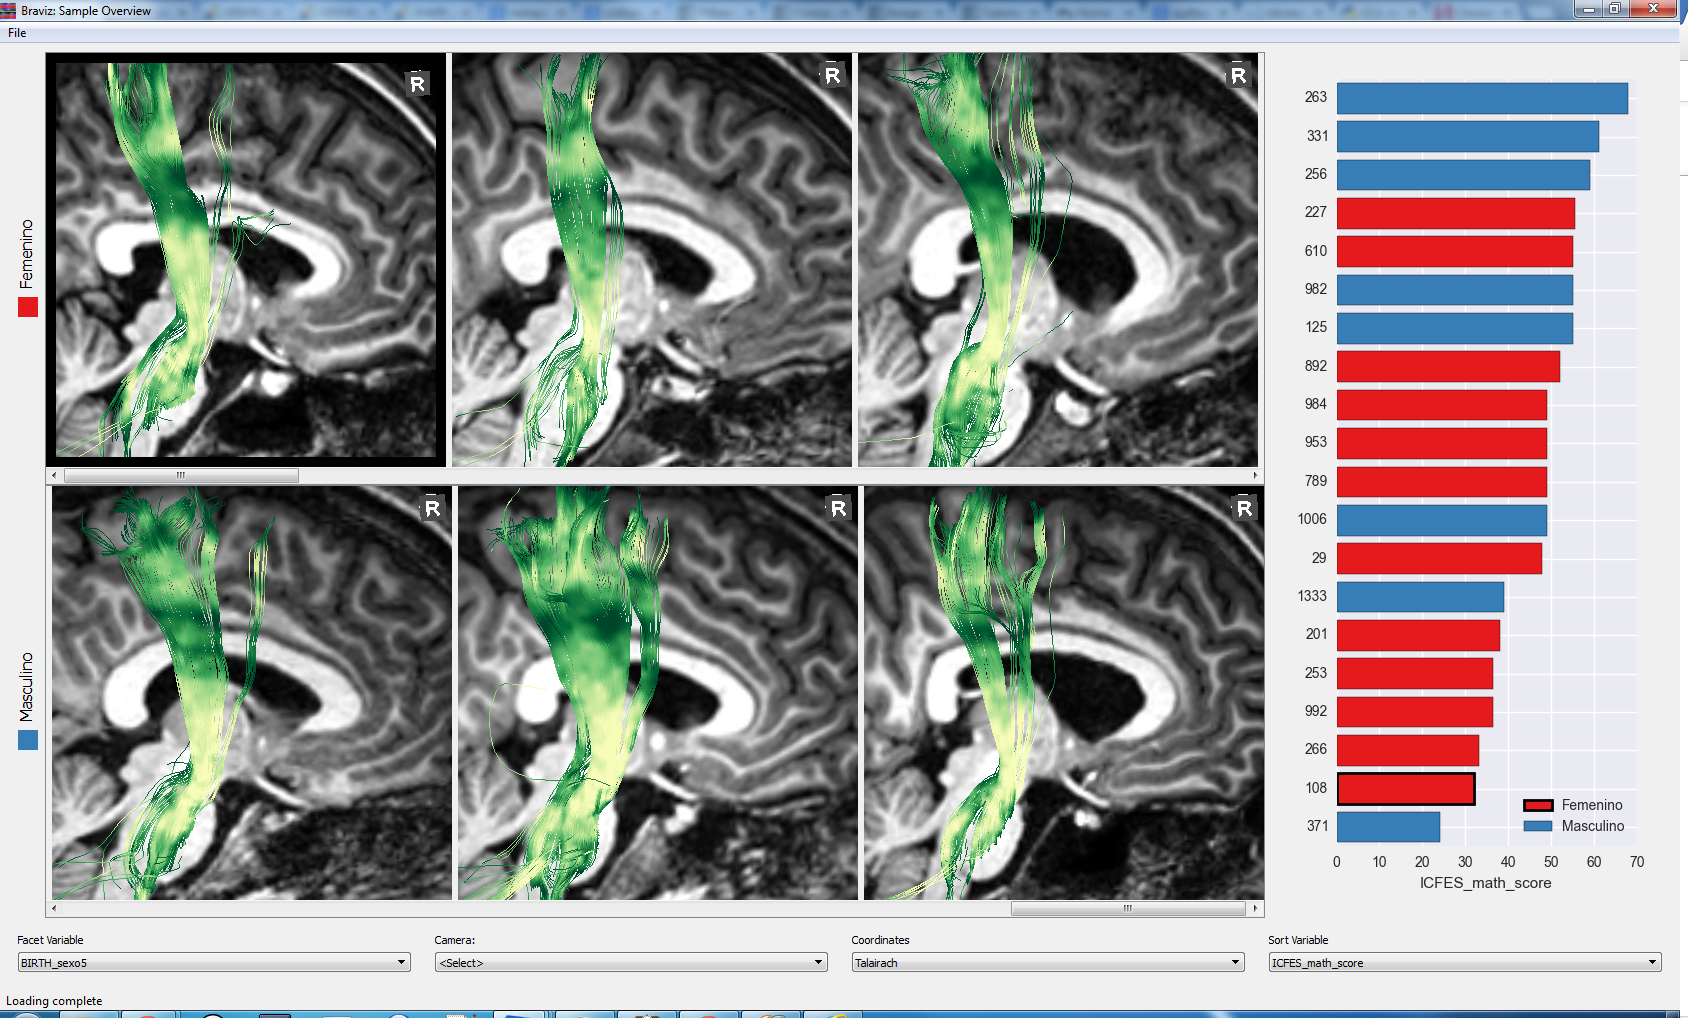
\includegraphics[width=0.9\textwidth]{braviz_qt/sample_overview.png} 
\caption{\label{fig_sample_overview_2}Multiple subjects can be visualized at the same time in small multiples, a nominal variables is used for rows and a numerical value for left to right order.}
\end{figure}

In order to select variables in all of the applications, dialogs similar to the one shown on figure \ref{fig_var_select}. This dialog shows a list of variables that can be filtered, and for each variable provides a description, a type and a plot. In the case of nominal variables the labels for each level are also shown, while on numerical value the expected range of the variable and the optimal value is shown. Notice that this information can be modified by the user. 

\begin{figure}
\centering
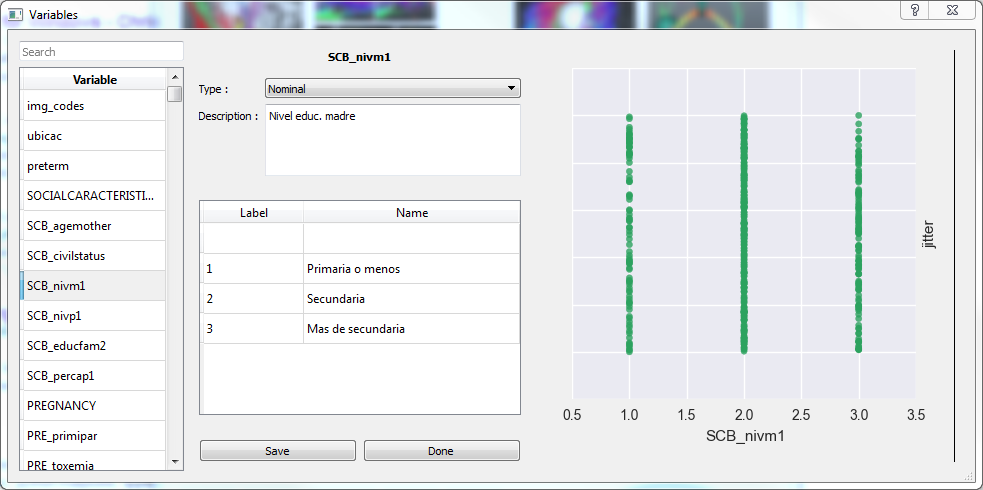
\includegraphics[width=0.9\textwidth]{braviz_qt/var_select.png} 
\caption{\label{fig_var_select}The standard dialog for selecting variables, notice the middle panel contains information about the variable while the right plot provides an overview.}
\end{figure}

The database of variables is a central component of this version, and as such we added features to perform typical statistical analyses on them without having to leave the platform. Figure \ref{fig_anova_2} shows an interface for performing anova  analysis using the data on the database. The user just selects an outcome, regressors, interactions and a sample. Samples can be created by filtering the population or other samples. An important advantage of doing the analysis here is that points in plots are also coordinated with other applications. This means that it is possible to right click on a point in a plot and make all currently open applications focus on that subjects, this includes the \emph{subject overview} application.

\begin{figure}
\centering
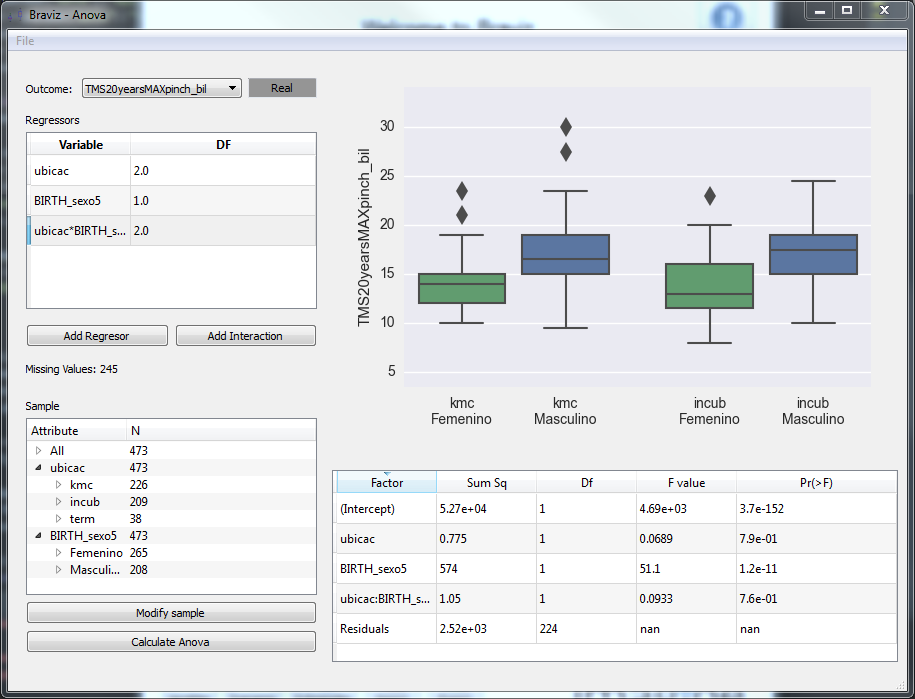
\includegraphics[width=0.9\textwidth]{braviz_qt/anova.png} 
\caption{\label{fig_anova_2}Anova analyzes on the variables in the database can be performed and visualized on this application. Data-points in the plots are coordinated to all other open applications.}
\end{figure}

Figure \ref{fig_lm_2} shows a similar application tuned for linear regressions. In this nominal variables are encoded using dummy variables, and the effects of each variable can be analyzed in the presence of the other variables. 

\begin{figure}
\centering
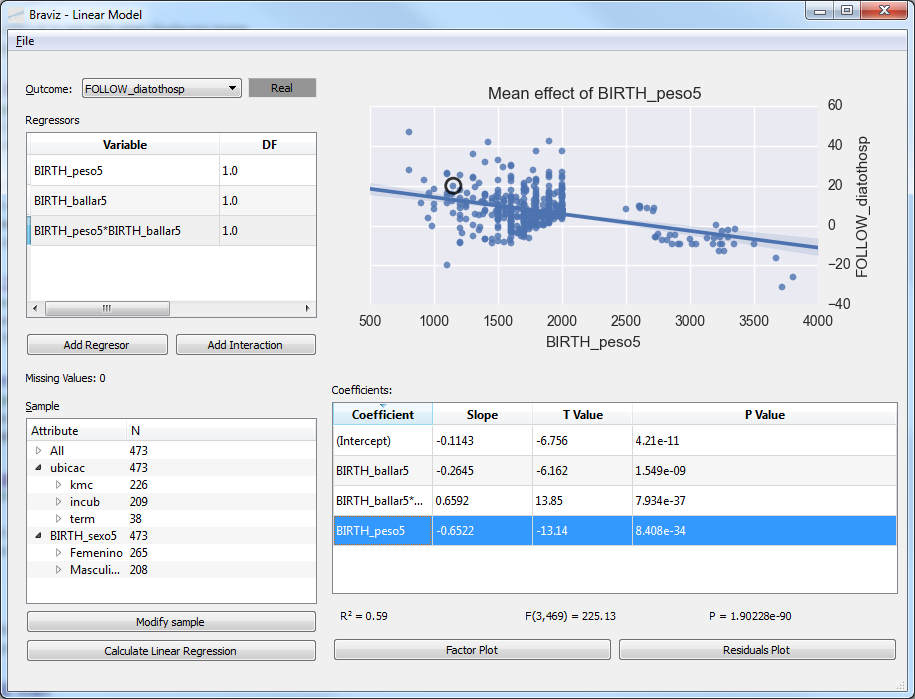
\includegraphics[width=0.9\textwidth]{braviz_qt/linear_model.png} 
\caption{\label{fig_lm_2}An application for fitting linear models on the variables on the database, the effect of one variable after correcting for the others can be visualized. Notice the highlighted subject in the plot.}
\end{figure}

Finding correlations between variables is a common task for researchers, and thus we developed the application shown in figure \ref{fig_correlations}. It features a correlations matrix in the middle, on the left side is a list of all variables in the project which can be added or removed from analysis with a click. Finally, when the user clicks on a square of the matrix a scatter plot of the two variables is shown at the right. This scatter plot also allows users to select a point and see the corresponding subject on other views, and it reacts to messages sent for this purpose from other applications. Another feature is that individual points can be added or removed from the sample just by clicking on them, in this way anormal points that have a large influence on the regression can be temporarily removed from the analysis. The reduced sample that is created trough this process can be shared to other applications to perform other analysis.

\begin{figure}
\centering
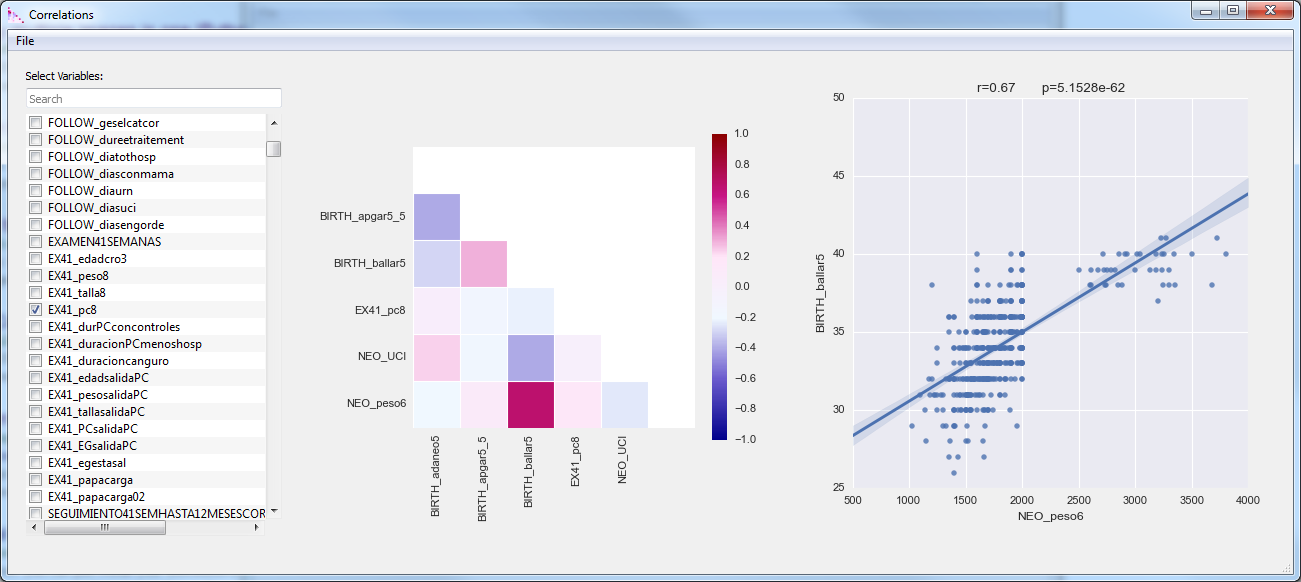
\includegraphics[width=0.9\textwidth]{braviz_qt/correlations.png} 
\caption{\label{fig_correlations}With this application it is straightforward to analyze correlations between variables.}
\end{figure}

The fMRI viewer from the previous iteration was upgrade to the one shown on figure \ref{fig_fmri_2}. This new version now loads complex experiment designs and contrasts directly from SPM files, which gives instantaneously an intuition of experiment structure, and makes mistakes evident. The new application also lets the user select multiple timelines at the same time, group them together, and make comparisons between groups. 

\begin{figure}
\centering
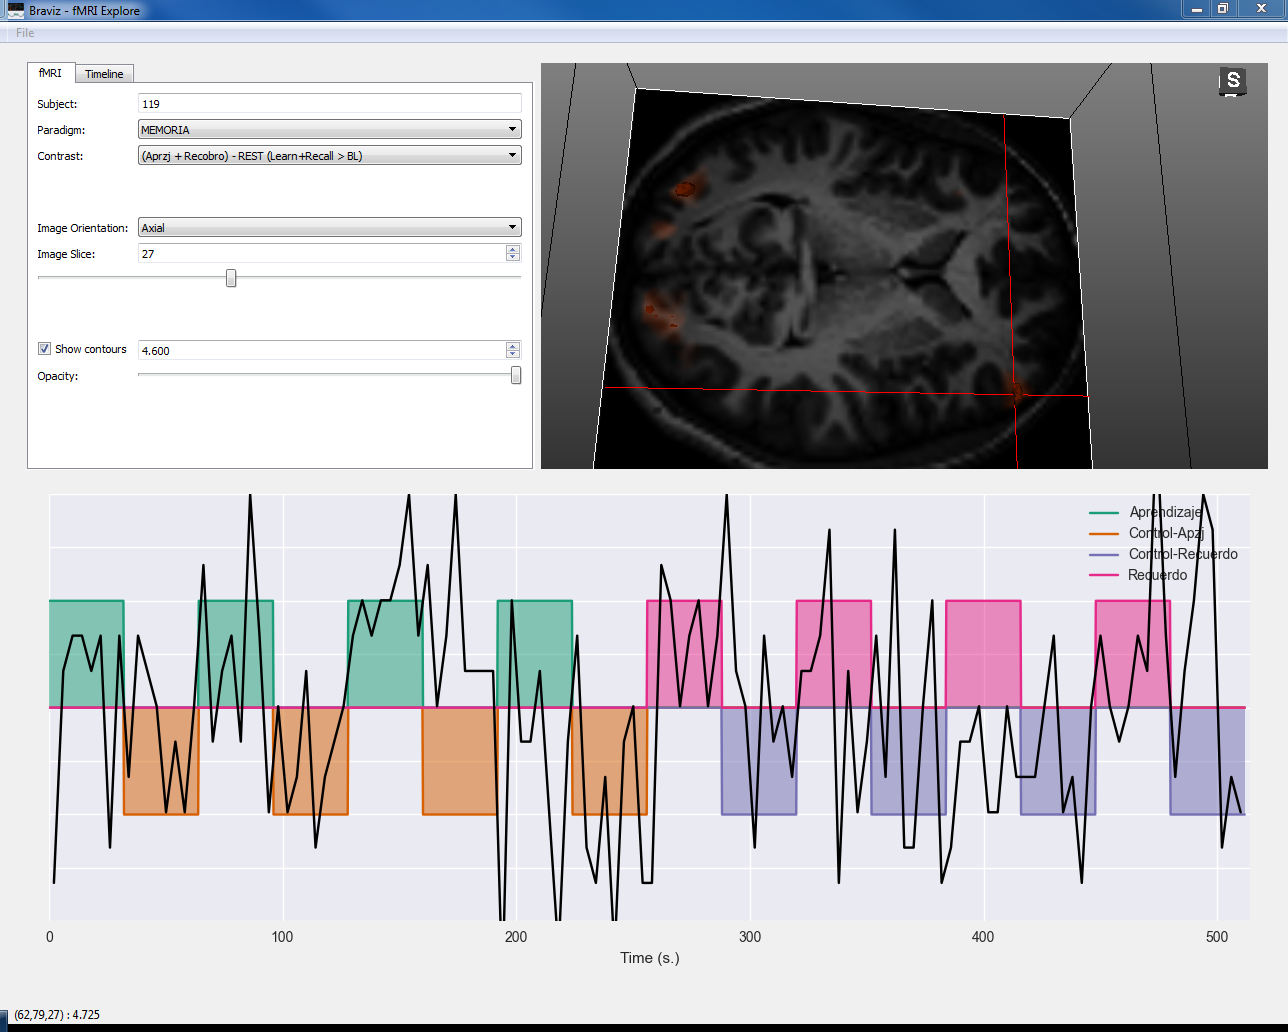
\includegraphics[width=0.9\textwidth]{braviz_qt/fmri.png} 
\caption{\label{fig_fmri_2}New version of the fmri explorer, now more complex experiments can be analyzed and timelines from different locations and subjects can be saved and compared.}
\end{figure}

While most of the applications of this iteration use QT for the graphical interface, we were also interested in web based technologies. Figure \ref{fig_parallel_2} shows a parallel coordinates view of the variables in the database created with the D3 \autocite{bostock_d$^3$_2011} javascript library and running on a web browser. Each line on the visualization represents a subject, while each axis represents a variable. Even though this application is running on a web browser, it is still possible to synchronize it with the rest of the system. This means the user can right click on one of the lines and make all the other apps focus on that subject, and in the same way, a line will be highlighted when the user asks for so in any other application. The mechanisms for making this possible will be explained on section \ref{sec_tech}.

\begin{figure}
\centering
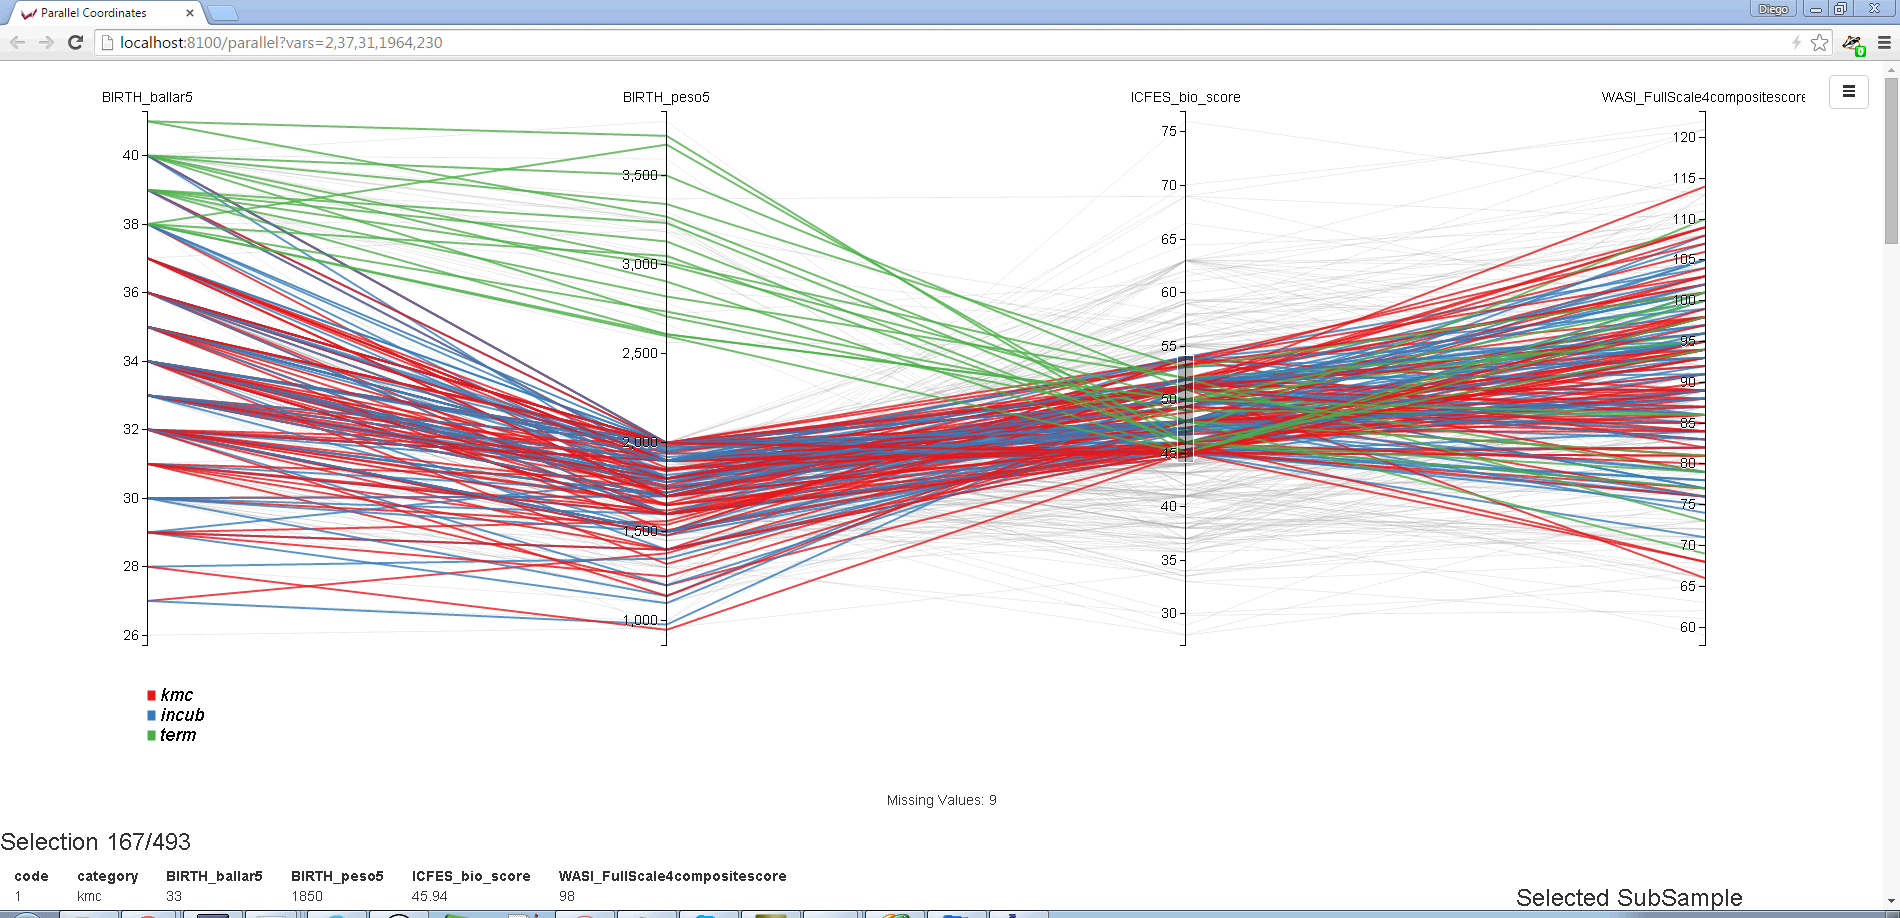
\includegraphics[width=0.9\textwidth]{braviz_qt/parallel.png} 
\caption{\label{fig_parallel_2}A parallel coordinates view of the variables in the database. Notice this visualization runs on a web browser.}
\end{figure}

Finally the menu, which acts as the entry point to the system, was also upgraded. Now in addition to the application launchers it includes utilities to import data into the database and export it, review and modify subsamples, look at the current variables and their meta-data, and review the saved states (scenarios) for all applications. From this last menu, it is possible to open any scenario, the correct application will then launch and load the saved state. Notice that the menu includes a first row with applications dedicated to manual or semi-manual measuring tasks. The objective of these applications is defining new geometrical structures or scalar measures that can be used in the rest of the system. It is possible to make linear measures on top of images, place spherical regions of interest based on images or surfaces while looking at the set of fibers that would result from that selection, and define custom fiber bundles by combining spheres and segmented structures trough logical operations. Examples of this will be given on chapter \ref{chap_kmc}.

\begin{figure}
\centering
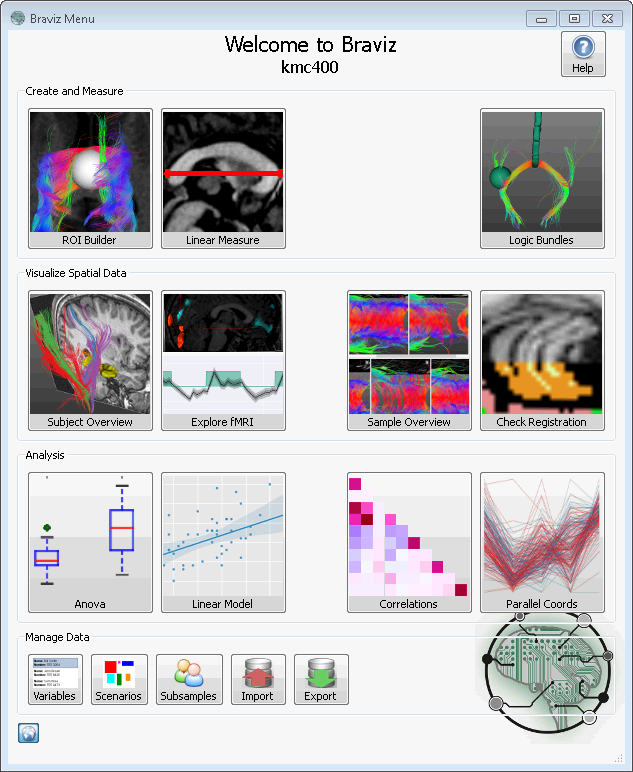
\includegraphics[width=0.4\textwidth]{braviz_qt/braviz_menu.png} 
\caption{\label{fig_menu_2}The menu for the new version of Braviz, notice the utilities on the bottom row.}
\end{figure}

% Sample applications
% Maybe recycle from paper , or from old draft on bitbucket


\section{Architecture}
\label{sec_arch}

%From model to implementation
%-----------------------------
%
%- architecture
%- common platform
%- coordinate system
%- skeleton of a application
%- database


Trough the user centered design process described in the previous section we arrived to the model described on chapter \ref{chap_model}. The proposal consists of a family of applications, each providing interfaces, visualizations and interaction mechanisms suited for specific tasks. However all applications share the same data and can communicate with other running applications. While they will be different from the user point of view, on the inside they share several operations, therefore it makes sense for them to share significant amounts of code. Another important requirement was that the whole system should adapt to different data storage mechanisms. 

The proposed architecture to implement these features is shown in figure \ref{fig_archi}. At the top of the diagram are the concrete applications. All of them make use of a library which provides all common braviz functionalities. Notice that each application can use a different subset of features from this library, as specified in figure \ref{fig_feature_solution}. In order to made the platform flexible, and adaptable to different data storage solutions, all data access operations are isolated trough the "`Project Reader"' layer. The current implementation uses files stored in disk, but we had used this layer to adapt to two different disk layouts. In the future this layer could be used to read spatial data from a database or web service. 

\begin{figure}
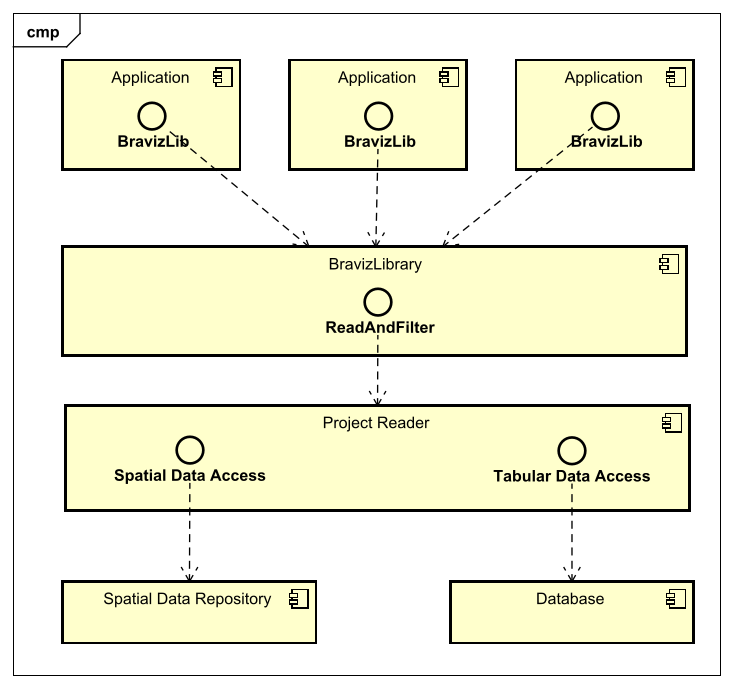
\includegraphics[width=\textwidth]{braviz/appArchitecture}%
\caption{\label{fig_archi} The architecture of Braviz Applications. The bottom of the diagram shows the underlying data storage, which is expected to be different for every project. The "`Project Reader"' layer serves as an isolation layer, when data storage mechanisms change only this layer needs to be adapted.}
\end{figure}

The library itself is divided into three modules

\begin{itemize}
	\item Read and Filter: Provides functions to access data and manipulate spatial data. This module loads the appropriate project reader based on a configuration file. However project readers themselves can use the other facilities in the module in order to transform the data into the expected format.
	\item Interaction: Provides re-usable widgets and interaction mechanisms, including communications with other applications in the family.
	\item Visualization: Provides several visualization elements, both for spatial data and tabular data.
\end{itemize}



\subsection{Read and Filter}

The \emph{readAndFilter} modules is in charge of providing the right data for all the other components. This mainly corresponds to the \emph{Data Sources} feature in\ref{fig_feature_solution}, and some basic \emph{Geometric Processing} operations, mainly related to data filtering and coordinate space transformation. 

Spatial data is exposed to the top layers via a declarative API; where the type of data, subject, coordinate system, and other parameters appropriate for the data type are passed to a function. Inside the function loads and applies all the required transformations. Each project reader must implement this API and must do the concrete operations required in the specific data-set to return the requested objects. Some examples of a call to this function can be seen in listing \ref{listing_read_and_filter_api}.

\begin{listing}
\inputminted{python}{code/read_and_filter_1.py}
\caption{Example of the Braviz spatial data reader API}
\label{listing_read_and_filter_api}
\end{listing}

The complete documentation can be found on the Braviz website. Notice that changing the coordinate system or the current subject is trivial if variables are used as arguments in all queries. Readers can also implement caching mechanisms in order to improve performance of future queries.  

Notice that it is possible to request specific sets of fibers by setting way-points in the query. This mechanism only supports getting bundles of fibers that cross several way-points or which cross any of them. More complex bundles can be requested by implementing specific functions inside the project reader, or by reading its description from the database. 

The types of data available for each project is not always the same. For this reason this method must also be able to inform applications which kinds of data are available. For this purpose most data types include an index parameter as can be seen on listing \ref{listing_read_and_filter_indices}.

\begin{listing}
\inputminted{python}{code/read_and_filter_indices.py}
\caption{Getting lists of available data}
\label{listing_read_and_filter_indices}
\end{listing}

Applications and functions from other modules may assume that this function exists and behaves as expected, and in this way applications that work across different projects can be built. This API can also be used in an interactive console in order fetch data on the fly.

Project readers themselves are likely to share several operations. For this reason the module provides reusable functions wrapping input and output, format changes, transformations between coordinate systems and computation of scalars.

The spatial data repository should not be writable by the Braviz system. In this way users won't fear altering their raw data while using Braviz, and the platform will be easier to use together with other systems. However there should be another location where the results from expensive operations can be stored in a persistent cache. 

Complementing this source of spatial data is a database which contains several objects which can be manipulated by end users. This include

\begin{itemize}
\item Variables values and metadata
\item Saved application state
\item Subsamples
\item Subject Annotations
\item User defined fiber bundles
\item User defined geometrical objects (ROIs, Lines)
\end{itemize}

The concrete way in which these objects are stored depends on the project, but all reading and writing into the database should also be limited to this modules. More details about the currently implemented schema will be given in section \ref{sec_tech}


\subsection{visualization}

The visualization module provides reusable interactive visualizations. These are divided in two families: spatial data viewers based on VTK and statistical data viewer based on Matplotlib or D3. 

Spatial data viewers are made from several \emph{managers} specialized for dealing with each of the different data types. All managers draw to the same renderer, but each of them keeps the objects associated to specific kinds of data. In order for the full viewer to behave correctly it is important to keep all managers in the same coordinate system and the same subject. The currently available managers are 

\begin{itemize}
	\item ImageManager: Displays an image in a plane. The user can click on the image to get the values and coordinates of the current voxel. The manager keeps track of the current image modality, orientation and slice.
	\item FmriContours: Displays contoures for fMRI statistical maps. The manager keeps track of the paradigm and contrast, and the level of the template. A custom lookup-table can be used to color the contours.
	\item Model Manager: Displays segmented structures. Keeps tracks of the available models and the currently selected models. Can also return scalar values associated to the current models, and allows specifying models by laterality ("`dominand or non-dominant"') or side ("`left"' or "`right"').
	\item SurfaceManager: Displays freeSurfer surface reconstructions and its associated scalars. As the model manager it can handle subject laterality. Users can click on top of the cortical surfaces and get the value of the associated scalar. 
	\item TractographyManager: Displays tractography bundles colored according to direction, fa, md or using one different color for each bundle. Bundles can be defined using a list of models joined by \emph{and} or \emph{or}, or loaded from the database. 
	\item TraculaManager: Displays tracula bundles as surfaces.	
	\item Others: spheres, lines, planes or other objects should be in separate managers.
\end{itemize}

Concrete viewers are created by adding the required managers and writing the code that coordinates them. Also not all of the available configurations of each manager need to be exposes. This provides flexibility to create a viewer fit for each application.


For statistical visualization a qt widget the library provides a qt-widget that can display scatter plots, box plots, bar plots, and others. All of these implement tooltips and context menus for each data point and the ability to highlight a subject of group of subjects in the plot. Statistical visualizations can also be created using javascript libraries, specially D3. This is achieved by serving pages and data trough the Braviz web server. More details will be given in section \ref{sec_tech}.

\subsection{interaction}

The interaction module provides communication between applications and access to data processing functions. Communications are achieved by installing a communications client on each applications, which connects to a server usually found on the main menu application. Applications send messages trough the client, which are then relied to all running applications. When a message is received the client lets the application handle it. Currently there are a few types of messages available, but the protocol allows easy extensions

\begin{itemize}
\item Subject: Indicates applications that they should switch focus towards a particular subject
\item Sample: Indicates applications that they should work with different sub-sample
\item Log: Communicates the system of important user actions that should be stored into the analysis log
\end{itemize}


Statistical data processing is achieved by calling \emph{R} functions trough the rpy2 interface. All associated \emph{R} code should is contained in this module. Currently the available operations are restricted to fitting anova and linear models and calculating the importance of each variable towards predicting another by using a random forest model. New functions will be added to this module as they are required by applications. 

Spatial data can be processed using VTK, python scientific libraries or both. Currently the module provides functions to calculate values of an image inside a surface and calculating geometric descriptors of surfaces as volume or lengths of main axes.

This module also provides several Qt models, dialogs and widgets that can be reused on applications. This includes dialogs for saving and loading samples and scenarios and for selecting variables. Models are available to represent samples and structures. Finally there are convenience widgets for common applications as selecting samples or selecting images and fMRI paradigms and contrasts.

\subsection{applications}

The applications that are currently part of the system are listed below, together with its main components. This will show how the variability of the system can be materialized into a wide arrange of applications. 

\begin{itemize}

\item \emph{Roi Builder}: Lets the user define spherical ROIs using images or cortices as context. It includes a 3D viewer which can display images in 3-orthogonal planes, brain cortices, a sphere and the fiber bundles that go trough the sphere. It can provide the mean value of an image inside the current ROI. ROI locations for different subjects can be approximated by making use of registered coordinate systems.

\item \emph{Linear Measure}: Lets the user make linear measures on top of an image. It provide a viewer with three orthogonal planes and a line defined on top of a certain plane.

\item \emph{Logic Bundles}: Lets the user define fiber bundles by combining ROIs and segmented structures with logical operations (\emph{and}, \emph{or} and \emph{not}). It provides a 3D viewer where the bundle can be previewed together with tree orthogonal planes and brain cortices. Scalars associated with the bundle can be calculated.

\item \emph{Subject Overview} (Figure \ref{fig_subj_overview_2}): Provides a fully configurable 3D viewer with images, segmented structures, fMRI contours, tractography, Tracula bundles and cortical surfaces. It can calculate scalars from bundles or segmented structures. Also provides annotations and values for the current subject on selected variables. Communicates to other applications when the current subject changes and responds to subject messages by switching to that subject.

\item \emph{Sample Overview} (Figure \ref{fig_sample_overview_2}): Provides multiple 3D viewers which are associated to different subjects together with a bar plot. The configuration of each viewer is copied from one created in \emph{Subject Overview}. Viewers are arranged in a grid where columns are levels of a nominal variable and sorted from left to right based on a numerical variable. Bars are connected to the corresponding viewer. By right clicking on a subject either on a subject or bar, it is possible to communicate to other applications that they should focus on it. The applications also reacts to subject messages by highlighting the given subject.

\item \emph{Explore fMRI} (Figure \ref{fig_fmri_2}): Includes a 3D viewer that shows an fMRI image and contours. At the bottom is a time-line which shows the current contrast and the bold signal associated with the current coordinates. It is possible to get this signals from multiple locations or multiple subjects. This signals can later be grouped together in order to compare patterns between groups. The application communicates subject changes and switches to a subjects when asked to by a message.

\item \emph{Check Registration}: Provides a viewer with a single plane where two different images can be viewed using a checkerboard pattern. 

\item \emph{Anova} (Figure \ref{fig_anova_2}): Lets the user fit Anova models based on variables in the database. Provides an statistical viewer that can show box plots, scatter plots or Anova diagnostics. By right clicking on a point in the plot the user can communicate to other applications that they should switch focus to the corresponding subject. When a subject message is received, the corresponding message will be highlighted in the plot.

\item \emph{Linear Model} (Figure \ref{fig_lm_2}): Lets the user fit linear models where nominal variables with more than two levels are encoded using dummy variables. It has a statistical plot that can show scatter plots, diagnostics or regression plots. The plot can be used for communications in the same way as the one in \emph{Anova}.

\item \emph{Correlations} (Figure \ref{fig_correlations}): Displays a correlation matrix with selected variables and scatter plots with correlation values. In the scatter plots subjects can be removed or added back to the analysis. The modified sample can be shared with other applications. The scatter plot also includes the communication properties of the \emph{Anova} plot.

\item \emph{Parallel Coordinates} (Figure \ref{fig_parallel_2}): This application provides a D3-based parallel coordinates display with variables from the database. Filters can be applied on each axis and the resulting sample can be shared with other running applications. It is also possible to right click on a line in order communicate other applications they should focus on that subject, likewise the application will receive subject messages and highlight the indicated subject.

\end{itemize}

All but \emph{Parallel Coordinates} are stand alone Qt applications. However in the future we expect to have more web based applications. Also notice all of them can save and restore their state from the database. Applications with a concept of sample can save and load samples into the database. They also provide access to the sample creation dialog where samples can be modified. Sharing samples to all applications requires explicit actions in the part of the user, as otherwise this could be disturbing. On each application users can choose if they always accept received samples, always reject them, or ask every time. 

Chapter \ref{chap_kmc} will show examples of how this applications are used in a real project. This will clarify the role each of them play and how instant communication can enhance analysis.

%¿Maybe a table indicating which features are used in each application?

%Show variability

\section{Technical Details}

\label{sec_tech} 

%Technical details
%------------------

%- libraries

This section provides an overview of the technical aspects of the current Braviz implementation. This section will describe the technologies used inside the current application and give details of how data is read and stored and how communications between applications is achieved. 


\subsection{Dependencies}

One of Braviz design principles was not reinventing the wheel. Fortunately several high quality, robust and open source tools for data analysis are available. We make use of third party libraries whenever we can, and stay focused on interaction and visualization. The consequence is that Braviz has a somehow long dependencies list. 

As mentioned before, the main language used for the implementation is Python. It was chosen because it lets us have a fast development cycle. The language is concise, which means less coding is required to implement a feature. Additionally because it is an interpreted language it is easier to debug, and features can be tried in the interactive console before writing long term code. Finally, several scientific, data management and visualization libraries are available, with a strong community behind them.

The full list of Braviz dependencies on python packages are

\begin{itemize}
\item numpy \autocite{van_der_walt_numpy_2011}: Python numerical library, provides high performance numerical arrays and vectorized operations between them.
\item scipy \autocite{jones_scipy:_2001}: Python scientific library, provides algorithms for spatial data processing, statistics and input/output of matlab files.
\item pandas \autocite{mckinney_data_2010}: Provides high performance data-frames, which are perfect for storing, exchanging and manipulating tabular data.
\item VTK \autocite{schroeder_vtk_1998} : The visualization Toolkit, provides a framework for rendering high quality interactive 3D graphics. It is the most popular scientific visualization library, therefore by using it we increase compatibility with other tools. It is written in C, but bindings for several languages are provided.
\item matplotlib \autocite{hunter_matplotlib:_2007} : Python plotting library. Provides a wide variety of plots that can be used interactively. 
\item seaborn \autocite{michael_waskom_seaborn:_2015} : Provides a high level API on top of matplotlib for creating high quality statistical graphics using data-frames as input. 
\item nibabel \autocite{brett_neuroimaging_2006} : Provides input and output from a large array of file formats found in the neuroimaging ecosystem, including freesurfer, and nifti.
\item PyQt4 : Python bindings for the Qt user interface framework. 
\item rpy2  \autocite{gautier_rpy2:_2008} : Provides communications to R \autocite{team_r:_2012} from python, allowing us to use powerful statistical processing algorithms implemented in R. 
\item pyzmq: Python bindings for the ZeroMQ \autocite{hintjens_zeromq:_2013} protocol for communications between application using ip.
\item tornado : A python web framework, provides a robust web server which includes a powerful implementation of web sockets. 
\item psutil : A python utility to get attributes of running processes, including how much memory they are consuming.
\item savReaderWriter : A python library for reading data from SPSS files.
\item xlrd : A python library for reading data from excel files.
\item XlsxWriter : A python library for writing data to excel files.
\end{itemize}

In addition to the mentioned python libraries, Braviz makes use of the following R packages.

\begin{itemize}
\item ARM \autocite{gelman_arm:_2015}: Used to \emph{standardize} data before fitting the linear model.
\item CAR \autocite{fox_car:_2015}: Used to fit the Anova model using type 3 sum of squares.
\irem randomForest \autocite{cutler_randomforest:_2014}: Used to fit a a random forest model to the data in order to calculate which variables are more effective at predicting the outcome of a given variable.
\end{itemize}

% Data preprocessing
\subsection{Data Preprocessing}

It was mentioned before that Braviz can be adapted to several types of input data. Nevertheless for the current implementation we are using the following protocol for pre-processing spatial data. After data acquisition all dicom files were translated to the lab and went the following process. Raw data was also visually analyzed and problems with the acquisition were detected early. In some cases it was possible to recall the subject in order to get a new image, but in others data had to be discarded.

Anatomical MRI was processed through the freeSurfer \autocite{dale_cortical_1999} recon\_all pipeline. This generates a segmented image and reconstructions and parcelations of the cortical surfaces. The pipeline also generates an affine transforms to the Talairach space and several scalar values for both the cortical surfaces and subcortical structures. Segmented structures were reconstructed using the 3D-Slicer model maker plugin \autocite{aucoin_modelmaker_2014}. 

SPM's Dartel \autocite{ashburner_fast_2007} workflow was used to generate a template brain based on 40 ananatomical images, as well as non-linear registration between the anatomical images of all subjects and the template. 

Functional MRI series were processed in SPM \autocite{friston_statistical_2006} using the anatomical MRI as reference. This included realigning images, registering to the reference, smoothing, time filtering, estimating a statistical model for each voexel and calculating the score maps for each contrast. At the end of the processing several images, in SPM normalized space are obtained together with transforms from this space to the anatomical reference space. Data from the image realign process was also analyzed, and when the amount of correction applied was larger than a threshold an alert was given. In this case the images would be visually analyzed by an expert in order to decide if they should be excluded from further  analysis.

Diffusion Weighted Images were processed using the Camino Tractography toolset \autocite{cook_camino:_2006}, together with FSL \autcite{jenkinson_fsl_2012} and Dcm2Nii \autocite{rorden_mricron_2007}. The first step was converting the Dicom series to a 4D nifti image, together with two text files describing the diffusion parameters of each volume using Dcm2Nii. These files were converted to Camino format, afterwards a tensor model was fitted, and  following that, an FA image was extracted. This image was then registered to the anatomical MRI using the FLIRT tool (part of FSL). A brain mask from the anatomical image was extracted using FSL's BET. This mask together with freesurfers' white matter mask, were brought to diffusion space using flirt and the previously calculated transform. The white matter image was then used to derive seedpoints for a tractography reconstruction. The tractography results were cleaned to remove streamlines outside the brain mask, and to delete small stream lines. Finally these results were converted to VTK-format. An rgb DTI image, the FA image and a MD image were also extracted.  

Diffusion weighted images were also processed using the Tracula \autocite{yendiki_fully_2009} pipeline, which is included in freesurfer. This algorithms combines a probabilistic diffusion model with anatomical priors in order to reconstruct the main brain pathways. The output of this process is an image for each bundle containing the probability of it going trough each voxel, a file containing the more likely locations of all bundles, and a series of scalar metrics for each bundle.

The scripts using for the processing of data in the KMC project are available at \url{https://github.com/imaginebog/kmc_proc}. The results of all processing algorithms were saved into disk together with raw data following a the same structure for each subject. Notice that this process was not straightforward, and several corrections had to be made along the way. In the future it is recommended to use dedicated pipeline managing software as NiPyPe \autocite{gorgolewski_nipype:_2011} or LONI \autocite{dinov_efficient_2009}.

\subsection{Reading Spatial Data}
%- data input/output
%- transformations
%- coordinate systems

%  Dibujo esquema base de datos
\subsection{Data Base Schema}

%- messaging protocol
\subsection{Communications Protocol}

%  License
\subsection{License}


\chapter{The Kangaroo Mother Care Use Case}
\label{chap_kmc}
\label{chap_kmc400}

The Kangaroo foundation contributed significantly to the development of this project. Their research methodologies and data-sets on preterm children were the basis for the development of BRAVIZ, which they tested and used. In return the IMAGINE team helped in managing and processing image data, and its integration with clinical data. This chapter provides details of this collaboration and shows how the BRAVIZ platform provides value in a real study. The full methodology and results from the kangaroo mother care studies are found in \autocite{schneider_cerebral_2012} and \autocite{charpak_final_2015}.

\section{Kangaroo Mother Care}

%cual es el problema?
Low birth weight (LBW) is a mayor cause of child mortality \autocite{wardlaw_low_2005}, and on those who survive it can produce long term sequels and impairments \autocite{nosarti_neurodevelopmental_2010}. 

Kangaroo mother care (KMC) was developed by Edgar Rey in 1978 \autocite{rey_rational_1983} as an alternative to the conventional care method for infants born with low weight \autocite{conde-agudelo_kangaroo_2003}. It was initially conceived to deal with the lack of incubators and high rate of infections. The treatment is made up of three components.

The first one is kangaroo position, where the child is placed on the mother's or father's (or someone else's) chest, skin to skin, in an upright vertical position as shown in Figure \ref{fig_kmc_position}. This keeps the baby warm, and provides positive stimulation to the babie's brain through all senses. In kangaroo position the baby hears the mother's voice and her heart beat, senses her smell, feels her skin ans sees her face and her environment \autocite{tessier_kangaroo_2003}. In addition, the mother receives the stimulation she needs to increase milk production \autocite{charpak_kangaroo_2005}. This positions is maintained until the baby doesn't tolerate it any more, which indicates that appropriate temperature regulation has been achieved. 

The second component is breastmilk nutrition every two hours. The goal is to obtain a weight gain rate similar to what it would be in uterus. If the baby's growth is shown to be adequate the feeding schedule can be relaxed. In case the target weight gain can't be accomplished with breastmilk alone, a formula supplement may be added. This supplement should be administered via dropper or spoon so that it does not interfere with breastfeeding reflexes.

The final component is an early discharge from the hospital, with proper followup. This has the benefit of keeping the child away from infections, as well as providing an environment where strong bonds between the child and his family are more likely to form \autocite{charpak_kangaroo_2005}. 

\begin{figure}
    \centering
    \begin{subfigure}{0.45\textwidth}
        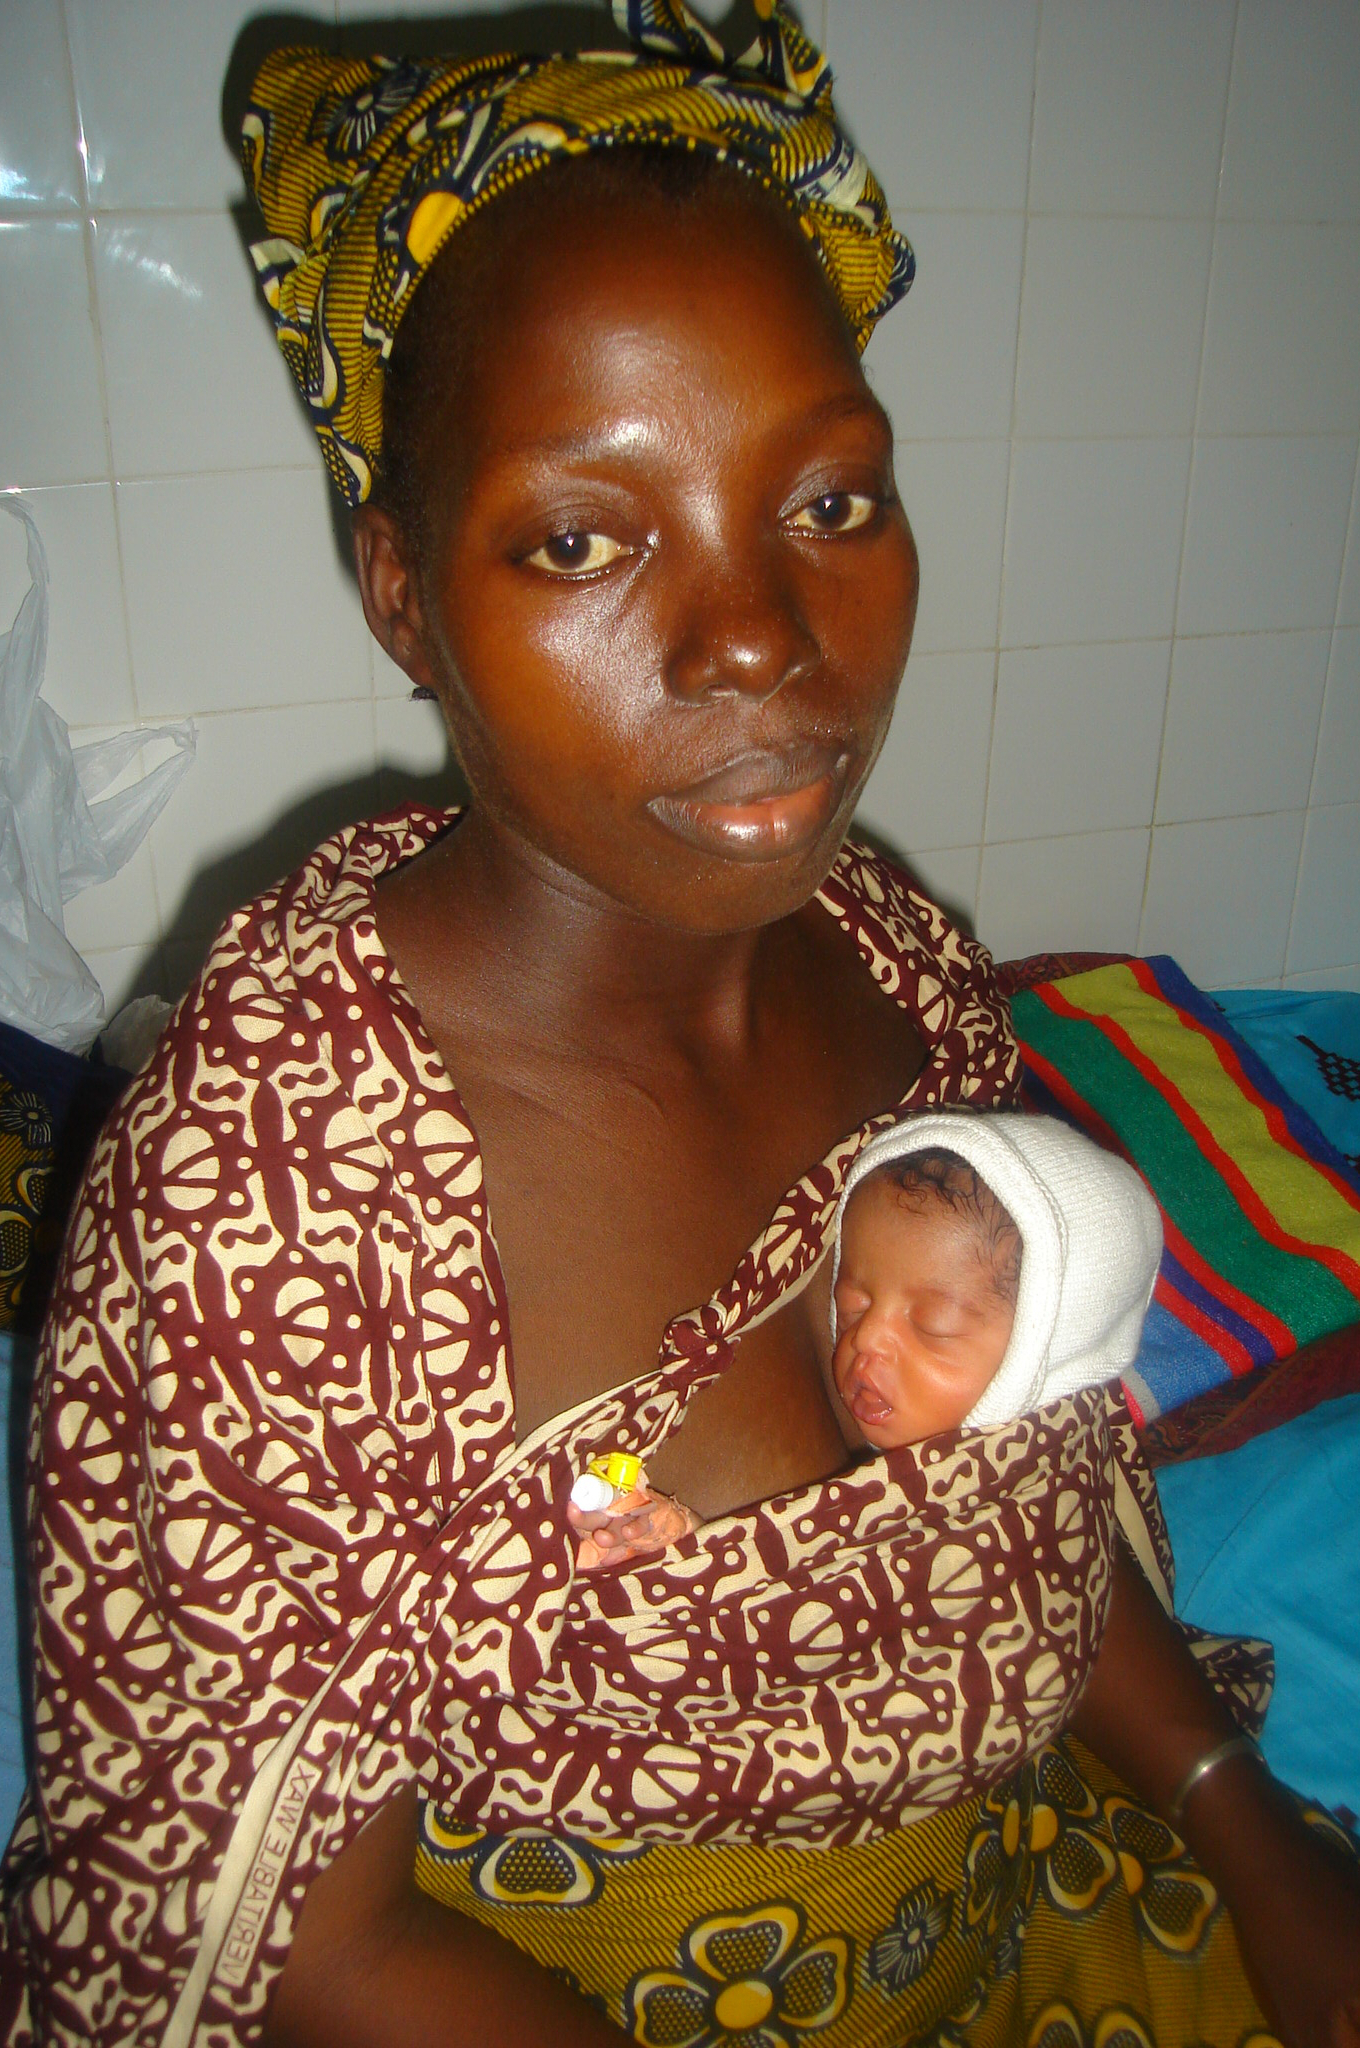
\includegraphics[width=\textwidth]{kmc400/221_trimmed}
    \end{subfigure} ~
    \begin{subfigure}{0.45\textwidth}
        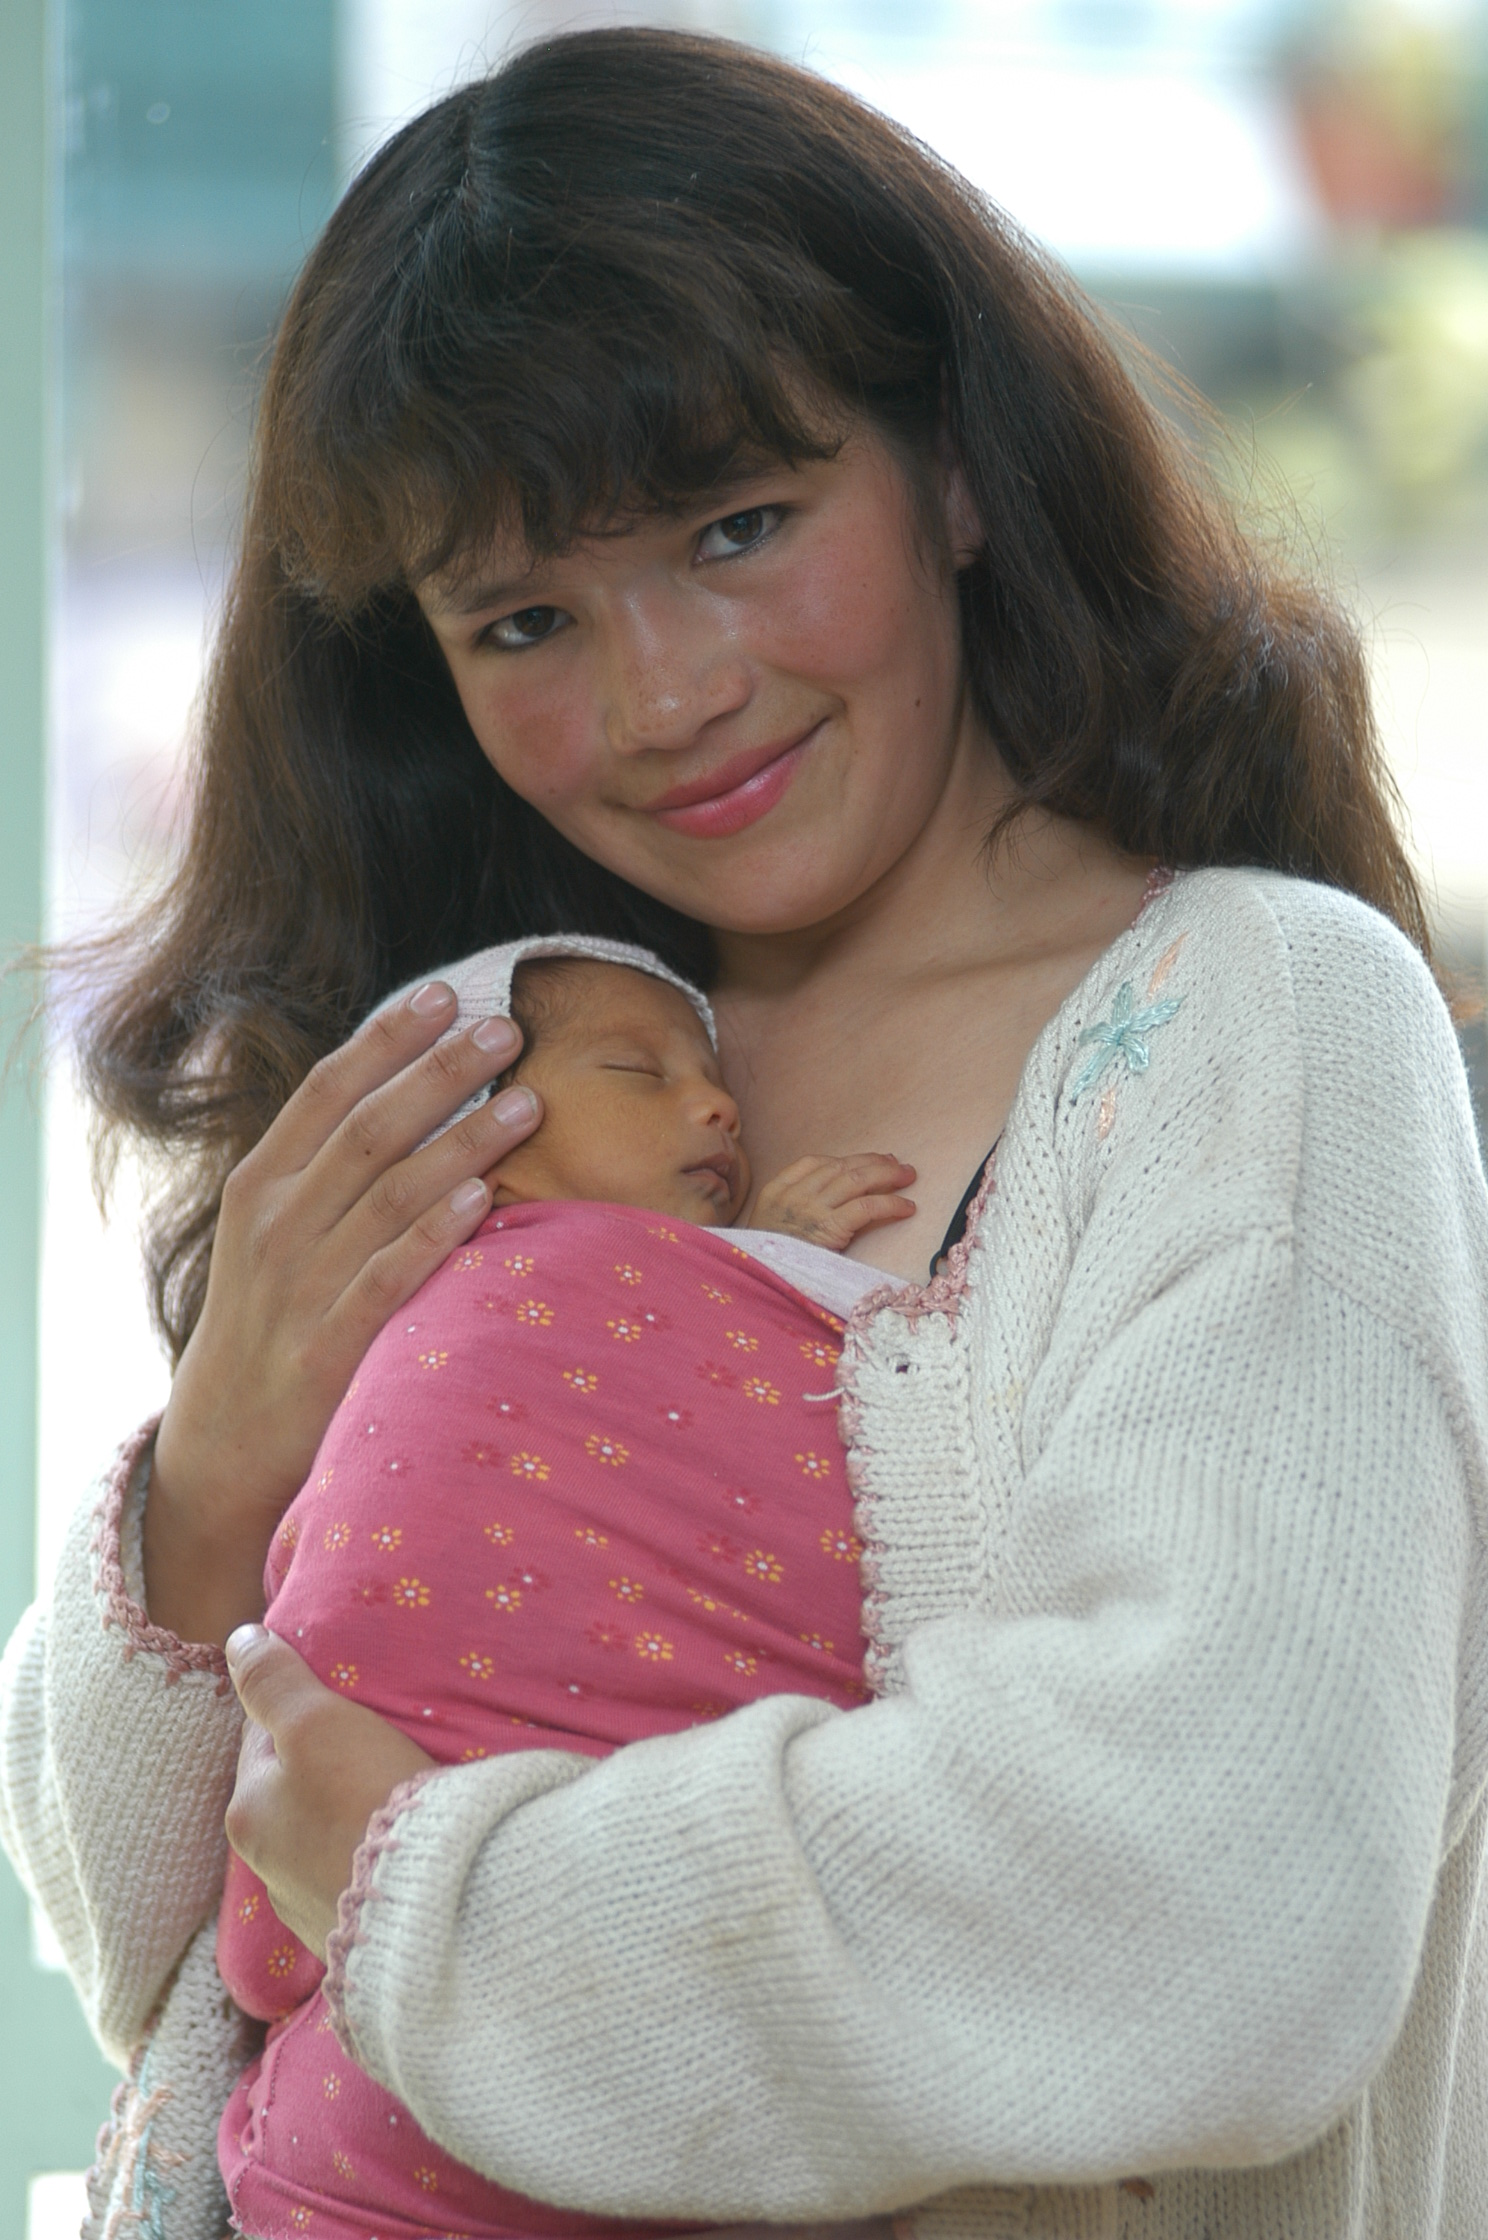
\includegraphics[width=\textwidth]{kmc400/0503canguro4d}
    \end{subfigure}
		\par \bigskip
		\begin{subfigure}{0.45\textwidth}
        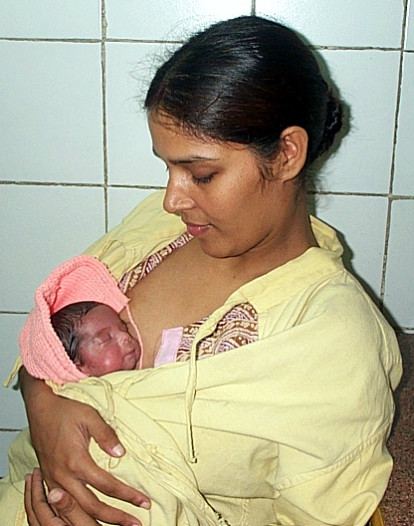
\includegraphics[width=\textwidth]{kmc400/Inde}
    \end{subfigure} ~
		    \begin{subfigure}{0.45\textwidth}
        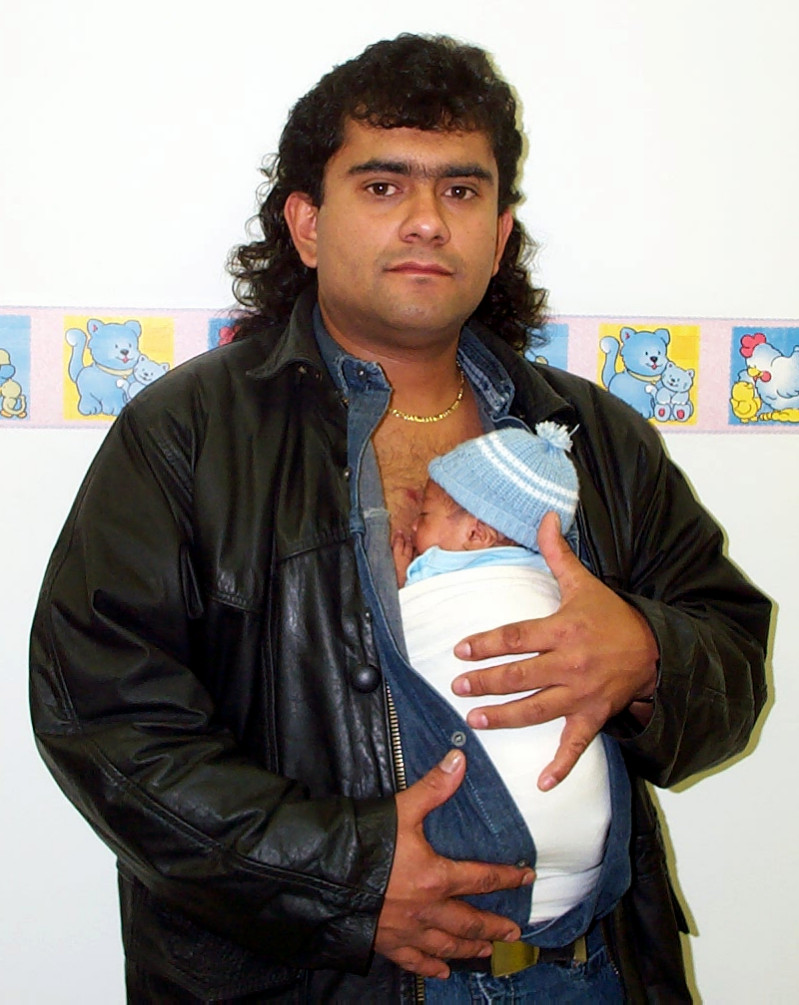
\includegraphics[width=\textwidth]{kmc400/papa2}
    \end{subfigure}
    \caption{Examples of the Kangaroo position, copyright belongs to the Kangaroo Foundation, used with permission}\label{fig_kmc_position}
\end{figure}

KMC has gone a long way since its invention \autocite{charpak_kmc_2011} and several refinements have been developed. For instance, the kangaroo position is now started as soon as the baby is born whenever its possible. Extensive research has been conducted on the method which has provided a better understanding of its benefits \autocite{the_cochrane_collaboration_kangaroo_2014}, and it  has been adopted by the world health organization as a major strategy to decrease neonatal mortality in low birth weight infants. The kangaroo foundation is present in 30 countries with 60 teams. 

%- What is KMC
%http://www.fundacioncanguro.co/en/quienes-somos.html
%(preguntar a Rejean y Nathalie)

\section{Randomized Control Trial}
%- The first randomized trial

A randomized controlled trial (RCT) was conducted between 1993 and 1996 to compare short and middle term outcomes of KMC in comparison to traditional treatment. The sample consisted of 746 infants born with low weight (less than 2000g.) at \emph{Clinica San Pedro Claver} in Bogotá. Eligible infants were randomly assigned to either KMC or traditional incubator treatment. KMC group remained on kangaroo position 24 hours a day and nurtured by breast feeding and an optional supplement (preterm infant formula) delivered by spoon or dropper, in order to guarantee a weight gain of 15 grams per kilogram per day until the reach of term. Children in the traditional group were kept in an incubator until they were able to control their temperature and were gaining weight at an acceptable rate, and discharged according to standard hospital practice. Both groups were followed until one year of corrected age. 

%-- What were the main findings
During this year there were fewer deaths in the KMC group as well as fewer visits to the hospital caused by infections. In addition, tests showed that mothers from the KMC group felt more competent with their babies. Griffiths and INFANIB tests showed higher cognitive development in the KMC group and this effect was more prominent on those born before 32 weeks of gestational age and those who went through ICU. There was also a high impact of KMC on the development of personal relations and on planning functions related to brain development \autocite{tessier_kangaroo_2003}. Details of this study and its findings can be found in \autocite{charpak_current_1996,charpak_kangaroo_1997,charpak_randomized_2001,charpak_kangaroo_2005}.


%\autocite{charpak_kangaroo_1997}
%\autocite{charpak_kangaroo_2005}
%\autocite{charpak_randomized_2001}
%\autocite{charpak_current_1996}

\section{Pilot Study}

%The pilot study
% - Data
% - TMS findings
% - IMAGINE

In 2009, thirty-nine children who were part of the original study were relocated. This sample was composed of children born at or before 33 weeks of gestational age, 21 belonged to the KMC group and 18 to the control group. In addition, 9 kids born at term at the same hospitaland with similar socio-economic background were recruited. 
The first step was performing full sight and hearing examinations and, in case of need, prescribing and manufacturing glasses or hearing aids. Then one month was given in order to let the children adapt to new glasses or hearing aids. 

Then they went through several neuropsychological tests including Wisc, VMI, and CBCL. 
Next a TMS experiment was performed where double pulse TMS was used to test intracortical inhibition and facilitation, and a single pulse was used to test interhemispheric inhibition. All measures were taken at the first interosseous, and both hemispheres were tested.
Finally magnetic resonance images (MRI) were acquired at \emph{Fundación Santa Fé de Bogotá} using a GE Sigma HD scanner of 1.5 Tesla. The protocol included structural T1 and T2 weighted images , DWI and six functional paradigms. 

%¿Que se hizo con estos datos?

%¿What tests?

%¿Resultados imágenes?

%¿Qué se hizo con las imágenes?

%¿Alguna otra publicacion?

Functional images were processed with FSL and DWI images were processed using MEDINRIA \autocite{toussaint_medinria:_2007}. Additionally several anatomical regions were segmented and measured manually. The KAB software platform described in section \ref{sec_kab} was developed to perform additional analyses on this dataset. This tool was appreciated by researchers as it provided a link between quantitative data and the spatial data from which it is derived. It also created an environment in which it was possible to think visually of the relationships between TMS, white matter structure and functional MRI. This dataset was also used for testing and validating the first versions of Braviz (see section \ref{sec_iterations}).

The TMS study in this pilot showed an important difference in kids that belonged to the incubator group compared to those in KMC and term \autocite{schneider_cerebral_2012} in inter-hemispheric inhibition. The latency of this inhibition also showed some interesting effects in the interaction between gender, hemisphere and group. This results indicate that KMC encourages brain plasticity and therefore reduce the negative effects of a preterm birth. 

% Parallel with braviz development in the previous section

\section{Saving Brains Project}

%Teams : images, psycho, economists, medical, eyes, social workers, 

% - Objectives
% - Data Collection
% -- Process
% --- how?
% --- when?
% -- Participants


%The saving brains project

Between 2013 and 2014, financed by Canada Grand Challenges, the kangaroo foundation started a project that involved relocating and recruiting 50\% of the subjects from the RCT that survived after the first year (between 340 and 430 subjects). Measures were taken in order to avoid selection bias in this sub-sample, specifically, comparing the distributions of relevant demo-graphical and clinical variables between the retrieved and not retrieved groups, as well as comparing them between the two groups (KMC and control) in the retrieved population. In case a selection bias was detected sensibility analyzes would be conducted on any results in order to mitigate the effects. 

Given budget restrictions it was not possible to perform magnetic resonance scans on the whole sample. However the initial RCT was stratified by birth weight, which allowed to make unbiased comparisons on each stratum. Therefore, it was decided to do imaging only on those participants which were born with less that 1800 g. 

By this time participants were between 18 and 20 years old. The study aimed at identifying if the KMC intervention had a long term effect protecting the brain against cognitive, social, and academic difficulties. Specifically, by analyzing data about brain maturation and structure, mental functions and behavioral patterns exhibited in family, school and work. 

Because there were no reference values for young adults available for some of the neuro-psychological and functional imaging paradigms that were to be acquired, a complementary sample of fifty subjects born at term on the same clinic where the RCT was performed was also retrieved. This sample was part of an observational study that occurred one year after the KMC RCT and i was meant only to provide reference values and not for direct comparisons with the other groups.

Relocating the subjects started by using the contact information from the original RCT; followed by searches in government databases and social networks, public media advertising and visits to the last known residency where information was sought from current inhabitants and neighbors. This labor was conducted by the social workers in the foundation, at the end managed to relocate 491 subjects, from which 441 could and were willing to participate in the new study. 


%phases of the study
\subsection{Data Acquisition Procedure}
 
As in the pilot study, the first stop for each participant is a vision and hearing examination, following by the prescription and acquisition of glasses or hearing aids if needed. After one month or habituation, data would be collected on tree different days.

The first day comprised a full medical evaluation where the medical history was collected and physical and neurological exams were performed by a pediatrician. During the exam, quality of life (Kidscreen-52) and Life habits surveys were administered. Subsequently a battery of neuro-psychological tests were administered by a psychologist. 

On a second visit the TMS experiment was conducted, and magnetic resonance images were acquired for subjects born with less 1800 g. of weight. 

Finally, the social worker and an economist visited the residency, place of work and school of the participant. In this visit an evaluation of the dwelling place was conducted, and questionnaires were applied to parents and best friend. If the subject was at school a class play test was performed in the classroom. Finally the economist retrieved information about the education and work history of the participant, and collected the necessary information and authorization to retrieve the results of the national high school test (saber-11).

In addition, data captured during the first year follow up were retrieved from the database. These included

\begin{itemize}
\item Social characteristics of parents
\item Pregnancy characteristics 
\item Type of birth
\item Weight, size and cranial perimeter at birth and during follow up
\item Hospitalization at birth and during follow up
\item Questionnaire of mother competence
\end{itemize}

Data was captured in paper and online using standarized forms. and then entered into an Microsoft Access Database specifically implemented for the project. Data cleaning and quality control processes were performed regularly during data acquisition. These included double data entry for selected variables and manual comparison of database values and raw data. Periodic exploratory analyzes were also conducted while data was being acquired. These allowed to quickly detect outliers and missing values, which could be caused by problems on data input. For this process SPSS was used together with BRAVIZ. The visualizations provided by the software and the capability of identifying individual points on plots provided an efficient way of detecting strange values.

Data acquisition for this project took about two years. After it was completed analysis of the data began. The first task was comparing demographic and biological variables from early life in the effectively retrieved sample with the full RCT sample in order to detect possible sampling bias. No problems were found at this stage. Afterwards \emph{crude} (unadjusted) comparisons were made for all metrics between the KMC and control groups. Then there was an analysis of possible confounders and effect modifiers (mediators and modulators); followed by the corrected comparisons between the two groups. 

Next, additional exploratory analyzis began. It is at this stage where BRAVIZ could make the most difference, especially when spatial data is to be considered. This process is not finished yet, and possibly there is much this data sets could tell. The following sections will take a closer look at the different dimensions of the study.

\subsection{Neuro-psychology and Environment}

In order to assess mental functions and behavior of subjects several neuropsychological tests were applied to participants. The majority were self-reports but some were filled by parents, best friends and classmates. The applied tests are listed below, full details are available at \autocite{uriza_reporte_2015}.

\begin{itemize}
	\item Cognitive
	\begin{itemize}
		\item WASI II: Abbreviated intelligence test
		\item TAP: Attention and memory test
		\item CVLT: Episodic memory
	\end{itemize}
	\item Life Quality
	\begin{itemize}
		\item Kidscreen: Health related quality of life questionnaire.
		\item Life habits questionnaire
		\item IPPA; Inventory of parents and peers attachment
	\end{itemize}
	\item Mental Health
	\begin{itemize}
		\item CES-D: Depression self report
		\item Conners: Attention deficit and hyperactivity disorders
	\end{itemize}
	\item Behavior
	\begin{itemize}
		\item ABCL: Adult Behavior checklist, completed by parents and best friend
		\item ASR: Adult Self Report
		\item Rosemberg: Self-esteem questionnaire
	\end{itemize}
	\item Neurosensorial 
	\begin{itemize}
		\item Edimburg laterality inventory: Dominant hand for multiple tasks
		\item Nine Holes Peg Test: Manual dexterity
		\item Beery Visuo-Motor Integration: Assesses integration between visual and motor abilities by copying images from a booklet.
		\item VMI: Visual perception and motor integration.
	\end{itemize}
	\item Environment
	\begin{itemize}
		\item Home: Family environment
		\item RCP: Revised Class Play, schoolmate relationship
		\item Evaluation of dwelling space
	\end{itemize}
\end{itemize}

The preliminary analysis of the data does not show any direct relationship of the treatment to any of the cognitive measures at adulthood. However it does show that during the first year there is a direct impact on the development quotient (DQ) measured by the Griffith. The hypothesis is that KMC creates positive changes in the family which have a direct implication on the DQ. At twenty years the IQ is highly related to the DQ at childhood and  environment variables (HOME), which are partially affected by the KMC intervention, as well as behavior and mental health variables. The working hypothesis is that KMC improves the familiar and home environment for the kid, which in turn creates a better environment for him to grow and develop, leading in the long term to a better performance in school and society.

\subsection{Economics}

The Research Group in Economics from Universidad del Rosario got involved in the project in order to analyze the education and labor history of the cohort, with the main question being if the KMC intervention affected these outcomes. For this purpose they created a questionnaire, based on validated questions from previous studies and the National Department of Statistics (DANE). This questionnaire was applied to each participant at the end of the domiciliary visit. The instrument also inquired about the schools to which the participant attended, the performance at those schools, and if currently the participant was studying or working, what kind of studies were they pursuing and what kind of work were they performing. Note that this study was approved by an ethics committee, where data protection measures were considered. The questionnaires were tabulated by a professional at the foundation and verified by the Economics group. Finally the results were merged with other variables of the study.

Additionally, participants gave their authorization to fetch the results of the last state high-school test (Saber-11) they completed. This test is applied to all students of the country when they are about to finish high-school, and it comprises sections on mathematics, language, social studies, philosophy,  natural sciences and English.

Analysis began by taking a broad look of the effect of the intervention on key variables, as the current wage and performance in Saber-11 using linear regression in the Stata software. At the next stage, the analysis was performed using additional variables as controls, chosen based on economics theory and previous experience of main researchers. This showed some interesting aspects in the results, which were discussed with the rest of the Kangaroo team. From this discussion, ideas of possible explanations and additional variables that should be taken into effect emerged. Ongoing work is analyzing specific subgroups inside the sample. 

Early results show that apparently KMC affects the way in which parents make choices, leading to KMC parents being more disposed to increase the number of years that children attend preschool. As many of the participants have not yet entered the workforce, results about wages can't be conclusive. Nevertheless an analysis restricted to those already earning a salary shows that KMC subjects have higher hourly wages. Additional analysis are still required to better understand the economical and educational outcome of this sample.  The complete discussion of the methodology and results from the Economics team will be published soon.

It is important that the analysis was carried out mainly through tables generated by Stata. Generating graphics in this software required additional steps, and therefore was only done to present the results. However when inquired about the possible benefits of using more graphics during the analyzes they expressed that they are used to reading tables and are very efficient at it, and usually, the amount of variables used in economics is limited and standardized. Nevertheless they appreciated BRAVIZ because it gave them access to spatial data, in which they didn't had any previous experience. They also recognized that interdisciplinary studies have much more variables than what they are used to, and therefore visual analysis will be very valuable for them in the future.


\subsection{Transcraneal Magnetic Stimulation}

%TMS details
TMS examination was carried out using two Magstim 200 stimulators coordinated by the Magstim Bistim. Subjects were comfortably sited in a chair with the arm in a pillow. An electrode connected to a EMG was connected to the first dorsal interosseus muscle. The TMS coil was located on top of the motor area of the opposed hemisphere. Optimal location for the coil was determined by the operator by searching the location that would induce a higher response on the EMG. For this procedure the stimulator was configured at 80\% of maximum output, if the hotspot could not be found at this level output power would be raised. The next step was estimating the motor threshold, this is, the minimum output power required in order to induce a response in the muscle on half the attempts. A test was next performed at 120\% of the threshold, this output would be used as baseline.

%	\begin{itemize}
%		\item Rest motor threshold
%		\item MEP (Motor Evoked Potential) Latency
%		\item Intra-cortical inhibition
%		\item Intra-cortical facilitation
%		\item Inter-hemispheric inhibition
%	\end{itemize}

Intracortical inhibition was tested by applying two pulses, the first one at 80\% of the threshold and the second one at 120\% of the threshold, separated by 3ms. For testing intracortical facilitation two pulses, at 80\% and 120\%, were used, but in this case separated by 15ms. These tests were repeated 10 times each, and performed on both hemispheres.

For testing interhemispheric inhibition the subject was asked to apply pressure with the thumb, first at maximum strength, and then maintaining it at 50\% of the maximum level. Afterwards a single pulse, at 200\% of the motor threshold , would be applied on the same side as the target muscle, this pulse would generate a response on the opposite side but also would cause an inhibition in the active muscle. 

%TMS processing
The signal captured by the EEG machine includes an artifact generated by the TMS pulse. An example signal can be seen in figure \ref{fig_tms_signal}. This signals are analyzed with the help of matlab scripts in other to determine the latency between the artifact and the motor evoked potential (MEP) or the inhibition; as well as the amplitude of the MEP in both cases, and duration of inhibition. Calculate the different in MEP amplitude between the baseline and intracortical inhibition or facilitation trials is a key measure. The time it takes for the signal to arrive from the motor cortex to the muscle is related to the distance it has to travel, therefore it is common to correct latency values with subject height. All these measures were calculated, averaged across all the trials, and added to the main study database.

\begin{figure}
	\centering
		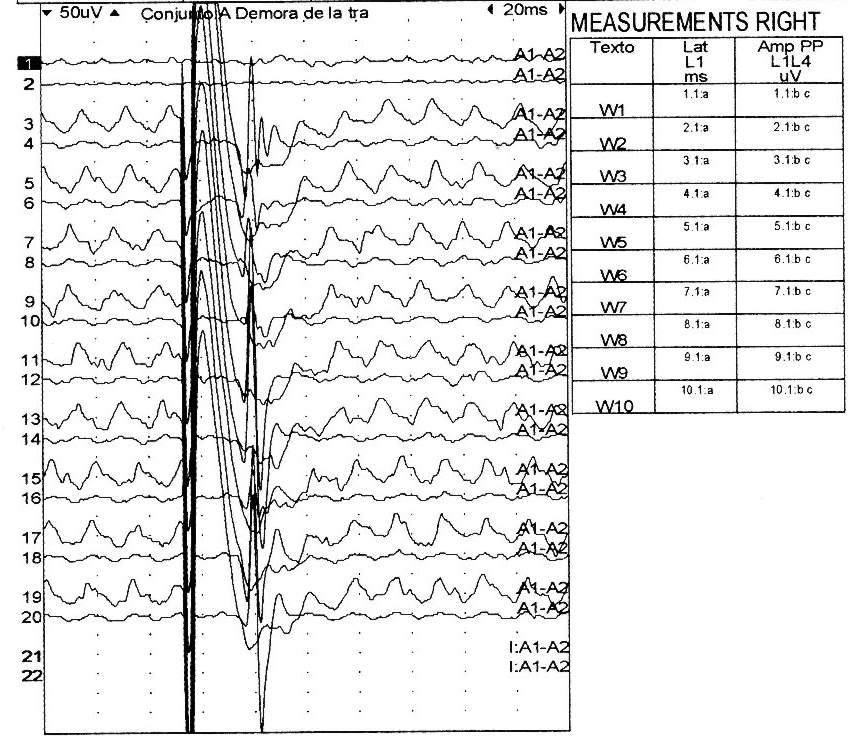
\includegraphics[width=0.5\textwidth]{figures/kmc400/tms_signal}
	\caption{A sample signal acquired during a TMS experiment.}
	\label{fig_tms_signal}
\end{figure}
 

\subsection{MRI Imaging}

%Autocite reporte interno Pablo y Felipe

% - Data Processing
% -- Pipeline
% -- Quality Control
% --- Early assessment
% --- Processing errors
% --- Pathologic Data
% -- Bundles Statistics
% -- Geometric descriptors

MRI image acquisition was done at the San Ignacio University Hospital using a Phillips Achieva 3 Tesla scanner with a eight channels head  antenna. A sequence resembling MPRAGE was captured in order to provide Freesurfer the most appropriate contrast for automatic segmentation. Additionally a volumetric T1 image and a Flair sequence and a T2 image were captured to provide additional anatomical context. A high quality diffusion weighted sequence was also captured as one of the main goals of the study was analyzing white matter structure. Tables \ref{tab_mri_params} and \ref{tab_fmri_params} show the detailed acquisition parameters used for each sequence. 
\begin{table}
	\centering
	\footnotesize
		\begin{tabular}{lrrrrr}
				\toprule
				Sequence&MPRAGE	&Flair	&T1 3D &DWI\\ 
				\midrule
				Sequence Type	&GR	&IR	&GR &SE\\ 
				Dimensions	&3	&2	&3 &2\\
				Slice width	&1	&5.5	&1 &2\\
				Repetition time	&8.52	&11000	&7.76 &8610\\
				Eco time	&4.13	&125	&3.724 &83.41\\
				Slice spacing	&1	&6.5	&0.5 &2\\
				Phase Encoding Steps	&251	&243	&220 &112\\
				Echo train length	&187	&31	&220 &59\\
				Filed of view	&74	&100	&100 &100\\
				Reconstruction	Diameter&250	&220	&220 &224\\ \addlinespace
				Dimension x &250	&1024 &448  &128 \\
				Dimension y &256	&1024 &448 &128 \\
				Dimension z &160	&23 &310 &70 \\ \addlinespace
				Voxel Size x	&0.97 &0.49 &0.21  &1.75 \\
				Voxel Size y	&0.97 &0.49 &0.21 &1.75 \\
				Voxel Size z	&1  &0.5 &6.5 &2 \\ \addlinespace
				Gradients   &    &    &    &    32 \\
				\bottomrule
		\end{tabular}
	\caption{MRI sequences acquisition parameters}
	\label{tab_mri_params}
\end{table}


\begin{table}
	\centering
	\footnotesize
		\begin{tabular}{lrrrrr}
	\toprule
	Paradigm &Attention	&Coordination	&Memory	&Grip &Fear\\ 
	\midrule
	Sequence Type	&GR	&GR	&GR	&GR &GR\\
	Volumes	&90	&90	&128	&125 &495\\
	Dimensions	&2	&2	&2	&2 &2\\
	Slice width	&3	&3	&3	&3 &3\\ \addlinespace
	Repetition time	&2000	&2000	&4000	&2000 &2300\\
	Eco time	&28	&28	&28	&28 &30\\
	Slice spacing	&3	&3	&3	&3 &3\\
	Phase Encoding Steps	&80	&80	&80	&80 &80\\
	Echo train length	&43	&43	&43	&43 &43\\
	Filed of view	&100	&100	&100	&100 &100\\
	Reconstruction	Diameter&240	&240	&240	&240 &240\\ \addlinespace
	Dimension x &80	&80 &80 &80 &64 \\
	Dimension y &80	&80 &80 &80 &64 \\
	Dimension z &40	&40 &40 &40 &32 \\ \addlinespace
	Voxel Size x	&3 &3 &3 &3 &3.8 \\
	Voxel Size y	&3 &3 &3 &3 &3.8 \\
	Voxel Size z	&3 &3 &3 &3 &3 \\
	\bottomrule
		\end{tabular}
	\caption{Functional MRI sequences acquisition parameters}
	\label{tab_fmri_params}
\end{table}

Five f-MRI paradigms were used in this study: Attention, coordination, memory, grip and fear. These paradigms were selected because previous studies  showed that preterm kids have motor, attention, memory and emotion management alterations \autocite{nosarti_neurodevelopmental_2010}. Because each participant could only remain inside the scanner for a limited time, not all paradigms could be applied to all subjects. Two groups were created, the first one went through grip, coordination, attention and memory; while the second one through grip, coordination and fear. 

The grip paradigm had a block design where subjects were asked to apply pressure with thumb on the side of the index finger, and in this way activating the first dorsal interosseus muscle, the muscle targeted in the TMS test. The coordination paradigm also had a block design but this time the task was opening and closing one or both hands following the pictures presented on the screen. The attention paradigm used a block design as well. In this case the subject would be presented with seven points on the screen, and they were instructed to follow the tree red points. Next all points would become black and start moving around the screen. At the end the initial points would become red again and the participant would be asked if they arrived to the same final position. 

The memory paradigm was composed of two stages, both in block designs. During the first stage participants were shown couples of words and asked to memorize them. During the second stage participants were presented with a word they have seen before, and two options for the second word. They were asked to identify which word was seen before together with the first word.


The fear conditioning paradigm was event related and divided in two stages. In the first stage participants were randomly presented with two woman faces. Half of the time one of the faces was shown was accompanied by a loud horror scream.  During the second stage  both faces were shown again randomly, but this time there would not be any scream. After the presentation of each face at both stages participants would have to respond using a qualitative scale how anxious they were feeling.
\smallskip

% Data analysis
\subsubsection{Spatial Data Analysis}

Image data was pre-processed as described in section \ref{sec_preproc}. Anatomical images went through a VBM analysis in SPM comparing the two groups from the randomized study, using age and gender as control variables and \emph{Eigenvariants} for each subject in each region of interest were extracted and added to the database of variables. MPRAGE images went through the FreeSurfer recon-all pipeline and all output statistics (volumes, cortical thickness, surface areas, and cortex curvature) were as well added to the database. 

At this points all of the spatial artifacts  generated by freesurfer (segmentations, transforms and cortex reconstructions) were also available in BRAVIZ, and therefore it was direct to use python scientific libraries to perform additional analyzes. Script that went through all segmented structures, and for each one calculated the main, second and third axes, as shown in figure \ref{fig_jth_descs} were run. The lengths of these axes were added to the database as new variables.

% JTHP descriptors
\begin{figure}
	\centering
		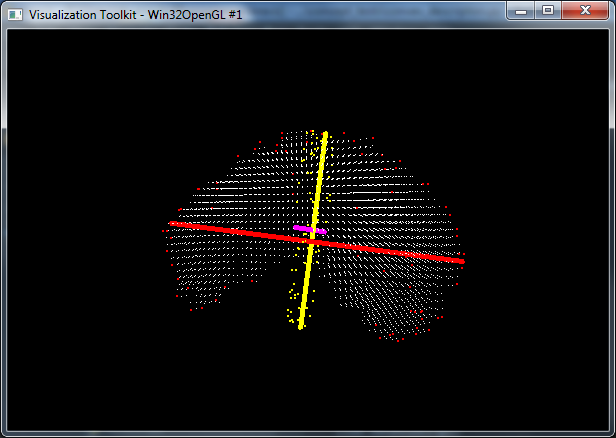
\includegraphics[width=0.9\textwidth]{figures/kmc400/desc_4}
	\caption{Illustration of the geometric descriptors calculated in python, white dots are the center of voxels that belong to a given structure, red points are those in the convex hull, the red line is the mayor axis of the structure, yellow points are the points in the structure projected to a plane perpendicular to the main axis, the yellow line is the mayor axis of this plane, finally the purple line is the axis perpendicular to the red and yellow axes.}
	\label{fig_jth_descs}
\end{figure}

DWI data was processed using Camino and the Free Surfer brain masks as references. Transformations between diffusion space and structural MRI space were calculated using \emph{FSL FLIRT}. From Camino, FA, MD and color DTI maps, were obtained together wit full brain tractography. All of these were integrated into BRAVIZ and made available for the experts. Using BRAVIZ based scripts, Free Surfer data was combined with tractography in order to isolate bundles going through particular structures. Mean FA, mean MD, mean length and number of tracks in these bundle were extracted.  While this could be achieved without BRAVIZ, it was certainly easier using the infrastructure provided by the software. Additionally BRAVIZ was used to let experts define spherical regions of interests and, based on them, define additional bundles of interest. The same scalar metrics mentioned before were extracted for these bundles. 

Free Surfer's Tracula pipeline was also ran on DWI images. Output statistics were exported into the database and the probability maps of the bundles were integrated into BRAVIZ for visualization. 

Functional MRI data was pre-processed in SPM.  After that a first level analysis was performed using specific contrasts for each paradigm, followed by a second level analysis using the main groups as regressor. The results from this analysis can be seen in \autocite{uriza_reporte_2015}. The BRAVIZ \emph{fMRI Explore} tool was particularly useful in the first level stage as it displayed contrasts in a direct and clear way. Figure \ref{fig_spm_contrast_error} shows a problem with a contrast, because the left and right conditions are not of the same length. This problem was quickly identified and corrected.

\begin{figure}
	\centering
		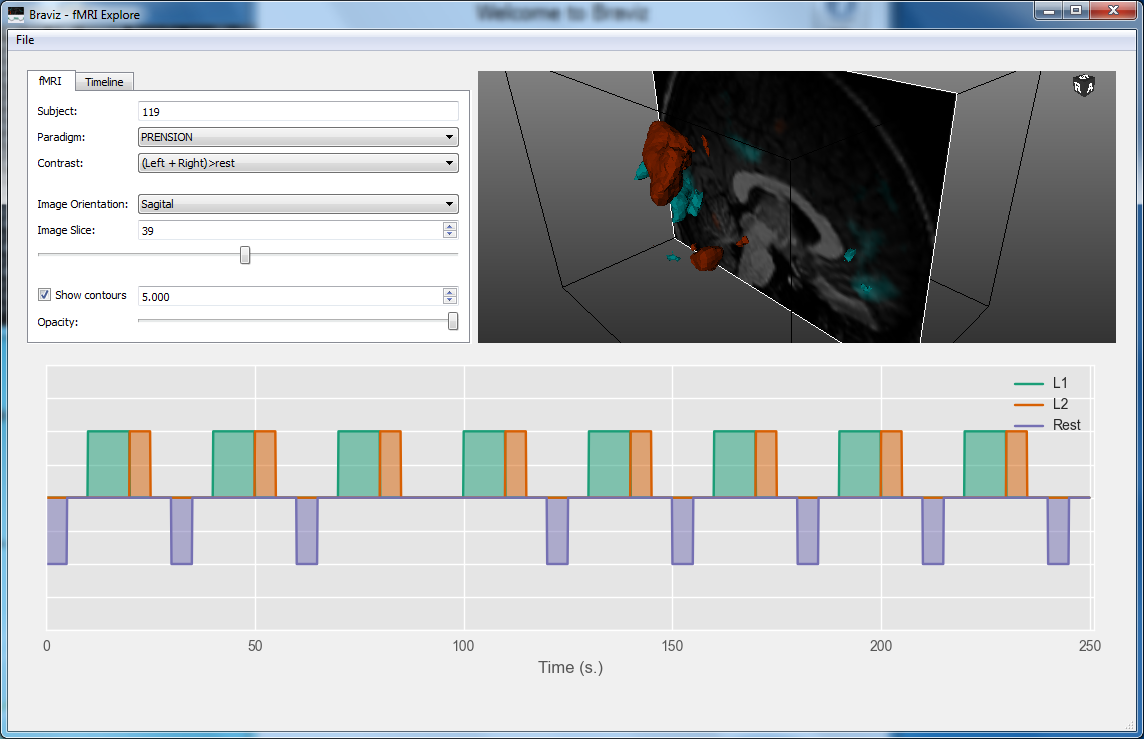
\includegraphics[width=0.9\textwidth]{figures/kmc400/erroro_fmri2}
	\caption{A problematic f-MRI contrast, L1 and L2 should have the same length.}
	\label{fig_spm_contrast_error}
\end{figure}
 

\subsection{Future Work}

The analysis of the data collected in this project is still far from finished. The crude analysis described above, which is simply regressing on each outcome variable against the exposition variable, is not enough. Reality is much complex and several factors must be taken into account to perform a meaningful analysis. It requires defining the sample carefully and choosing a meaningful set of confounders. Also it is interesting to look at relationships that don't include the exposure variables, in order to get a better understanding of the factors that affect the development of preterm kids. 

For the moment only basic analysis have been done on spatial data. The information that can be extracted using scalars is limited, and probably more interesting hypotheses can be discovered by making use of the totality of the data. However this will require advanced tools and methodologies. Several second level analyzes should be performed using the SPM framework, as well as TBSS analyzes and shape analysis. This will have to be complemented with visual analyses performed by domain experts and new visualization options that can work at this scale. It would also be interesting to analyze the raw data captured during the TMS experiments (EMG signals) in order to find additional patterns to the ones found using the derived scalars. 

Another challenge is looking at the behavior of the cohort through time. This is, analyzing the stability or variability of the different dimensions at the different epochs in which data is available, and looking at the factors which determine this changes.

All data collected during this study will be made available on request to interested researchers from around the world, with the objective of improving the understanding of the different factors that affected development of this cohort. This data must be used for hypotheses generation through exploratory analyzes, while confirming those hypotheses will likely require gathering additional data.

%Future
%Group analysis
%Mas analisis
%¿Se va a publicar la base de datos?


\section{Braviz Contributions}

%quality control
\subsubsection{Quality Control}

Gathering data and collecting it in a database in a project of this magnitude is large and complex task. Several steps are required and on each of them several things can go wrong. Data has to be continuously checked, validated and corrected as the project moves forward. This labor can benefit from automatic tools that check for values that are outside of range, are missing or which don't add up with other values. However large amounts of manual inspecting is also required. 

Anomalies in the data are much easier to detect when data is presented in graphical form than when presented in a table. A famous example of this is the Anscombe's Quartet \autocite{anscombe_graphs_1973}. BRAVIZ can be used to visually explore data even as it is been acquired. Visualizations can be created and re visited again when more data is available. By looking at plots from the data strange values immediately grab researcher's attention. This values can be instantaneously identified and verified from the raw data. Results from all analyzes are always accompanied by plots, which provides another sanity check. Any bizarre values will become evident and therefore the danger of believing results based on pathological data is drastically reduced.

Verifying image data is also simple using tools from Braviz. The setup used the most was several \emph{Subject Viewer} applications showing different critical slices of the image. An expert in radiology could then cycle through the subjects using the keyboard, and asses their quality. By using the platform it was possible to go over two hundred subjects in an hour. Images that appeared strange at first sight would be further evaluated by navigating in the 3d Viewer. Likewise quality of the registration between the different modalities could be checked by for example displaying the corpus callosum segmentation on top of an FA image or using the dedicated \emph{Check registration} application. 

%fibers analysis
\subsubsection{Fiber Bundles Creation}

As the project advanced, questions related to different pathways in the brain started to emerge. In order to answer these questions it was necessary to isolate in the tractography specific fiber bundles. Some of these could be defined using structures segmented by FreeSurfer, and therefore easily extracted for all subjects. However some of them required more precise location of regions of interest. 

The \emph{Roi Builder} application was created to streamline the placement of ROIs for each subject. An expert can specify the precise location for a region of interest in a single subject, using diffusion, structural and functional images, and results from segmentation as a basis. By having all images together in the same space, the correct location for the ROI can be better determined. Figure \ref{fig_thalamus_seed} shows how the lateral thalamic region can be seeded using three different image modalities.  This application also permits using additional region of interests to better isolate an specific group of fibers. This can be seen in Figure \ref{fig_thalamus_fibers} where the bundles from the lateral thalamus to the medial cerebral peduncle are isolated by using two different spherical ROIs. 

\begin{figure}
\centering
	\begin{subfigure}{0.3\textwidth}
		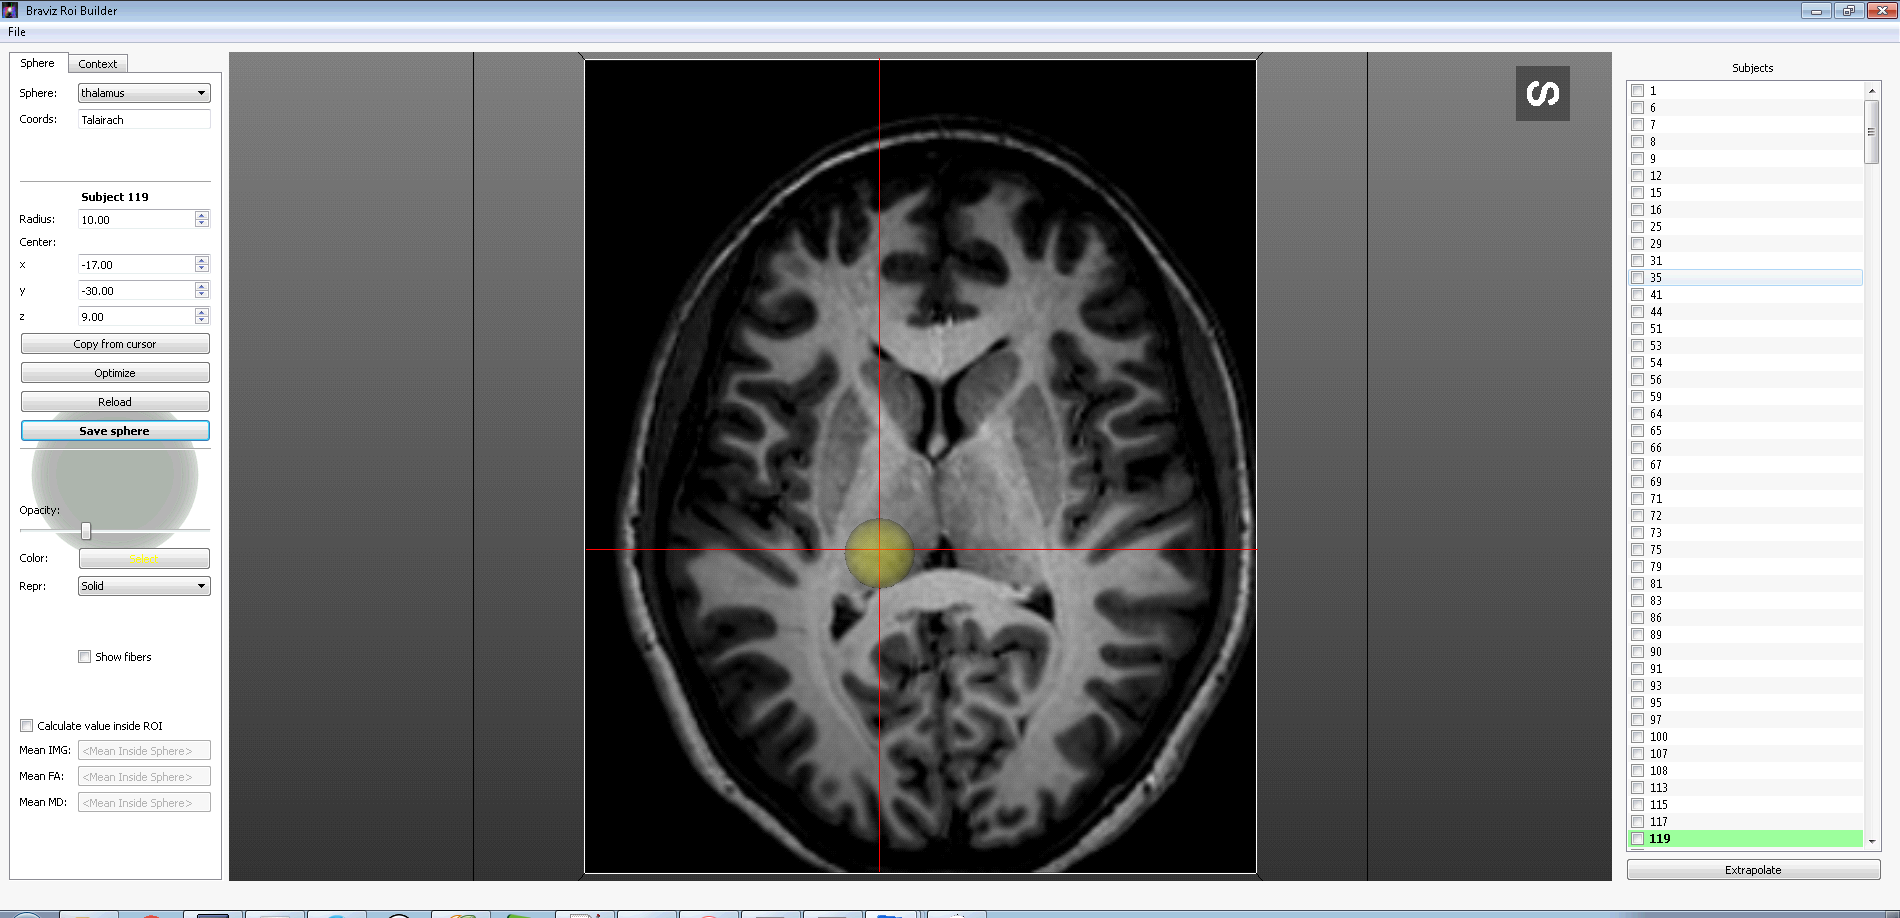
\includegraphics[width=\textwidth, trim = 450pt 50pt 500pt 100pt, clip]{kmc400/thalamus_mri}
		\caption{T1}
	\end{subfigure}
	\begin{subfigure}{0.3\textwidth}
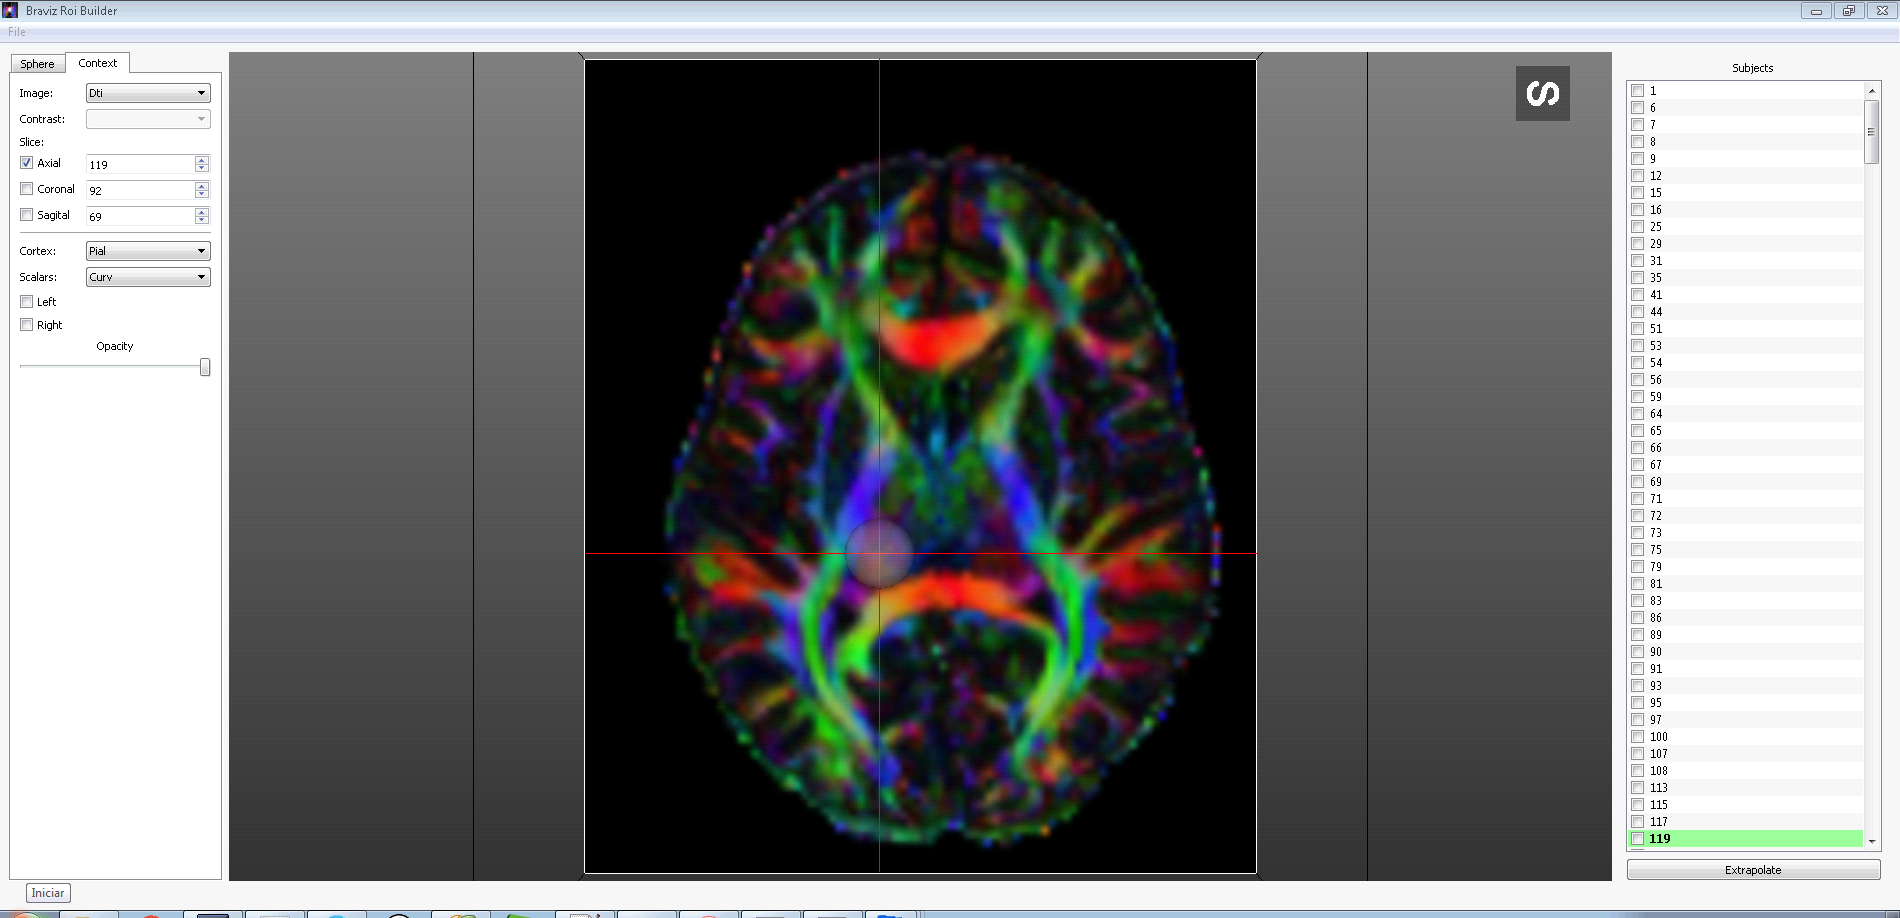
\includegraphics[width=\textwidth, trim = 450pt 50pt 500pt 100pt, clip]{kmc400/thalamus_dti}
		\caption{DTI}
	\end{subfigure}
	\begin{subfigure}{0.3\textwidth}
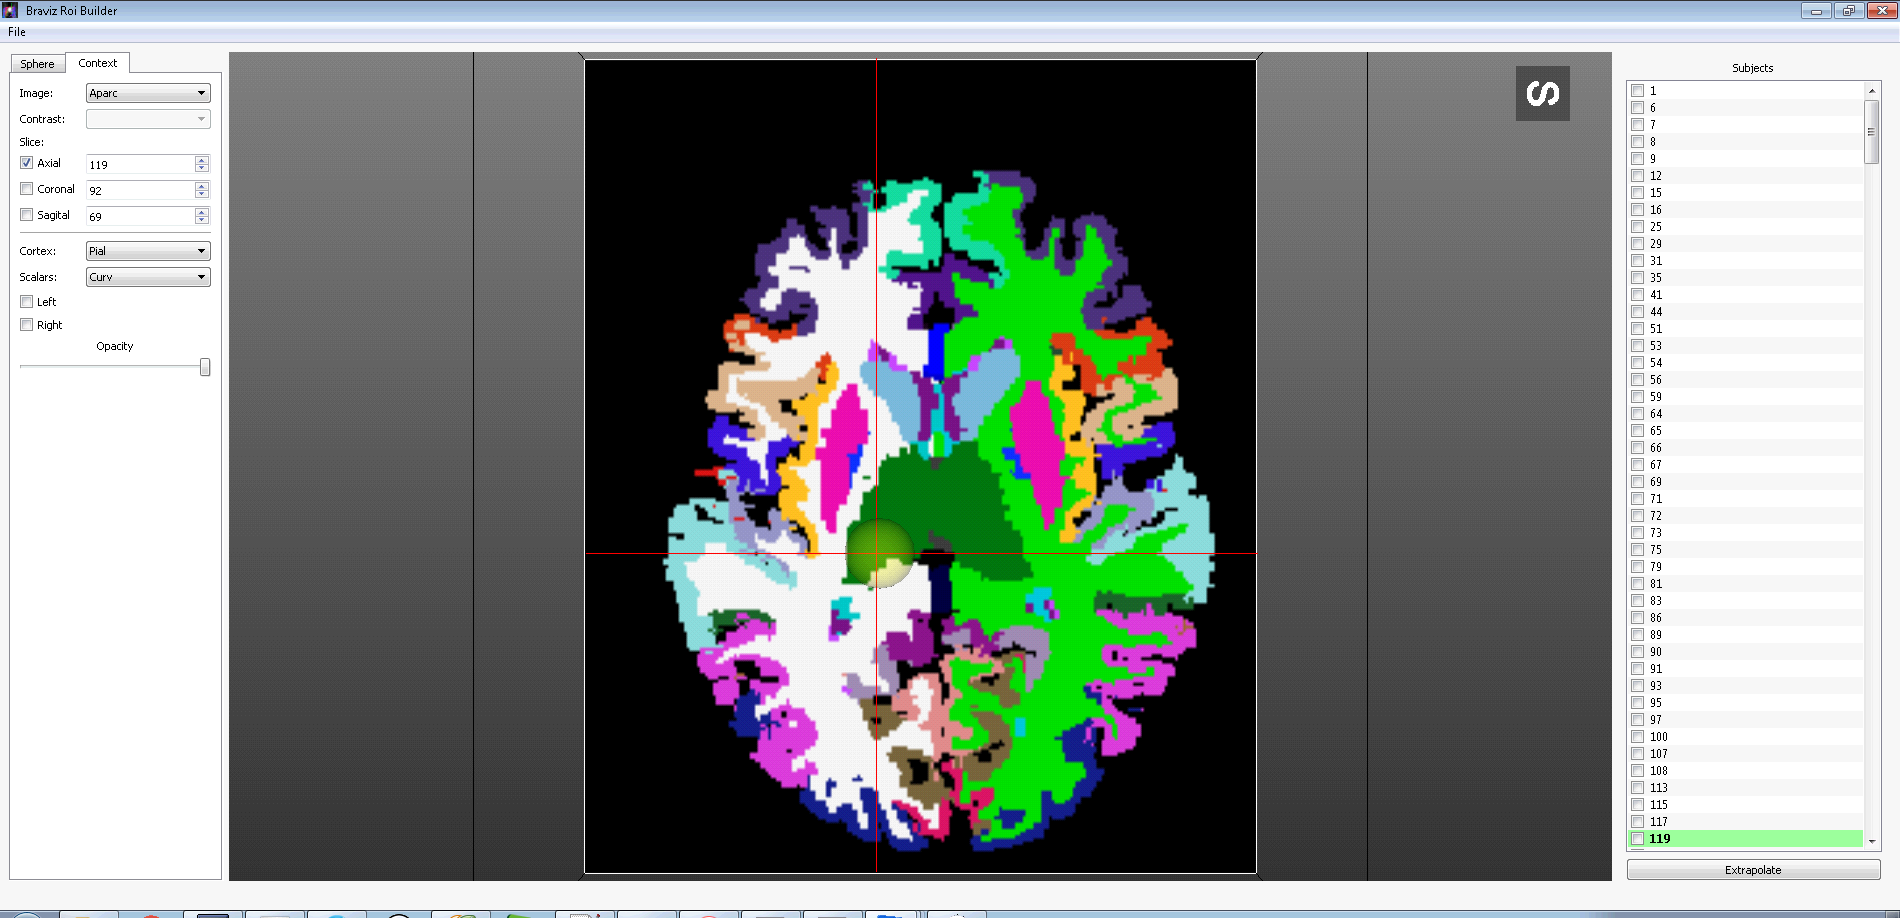
\includegraphics[width=\textwidth, trim = 450pt 50pt 500pt 100pt, clip]{kmc400/thalamus_aparc}
		\caption{APARC}
	\end{subfigure}	
\caption{Placing a region of interest in the lateral thalamic region
\label{fig_thalamus_seed}}
\end{figure}



\begin{figure}
\centering
	\begin{subfigure}{0.45\textwidth}
		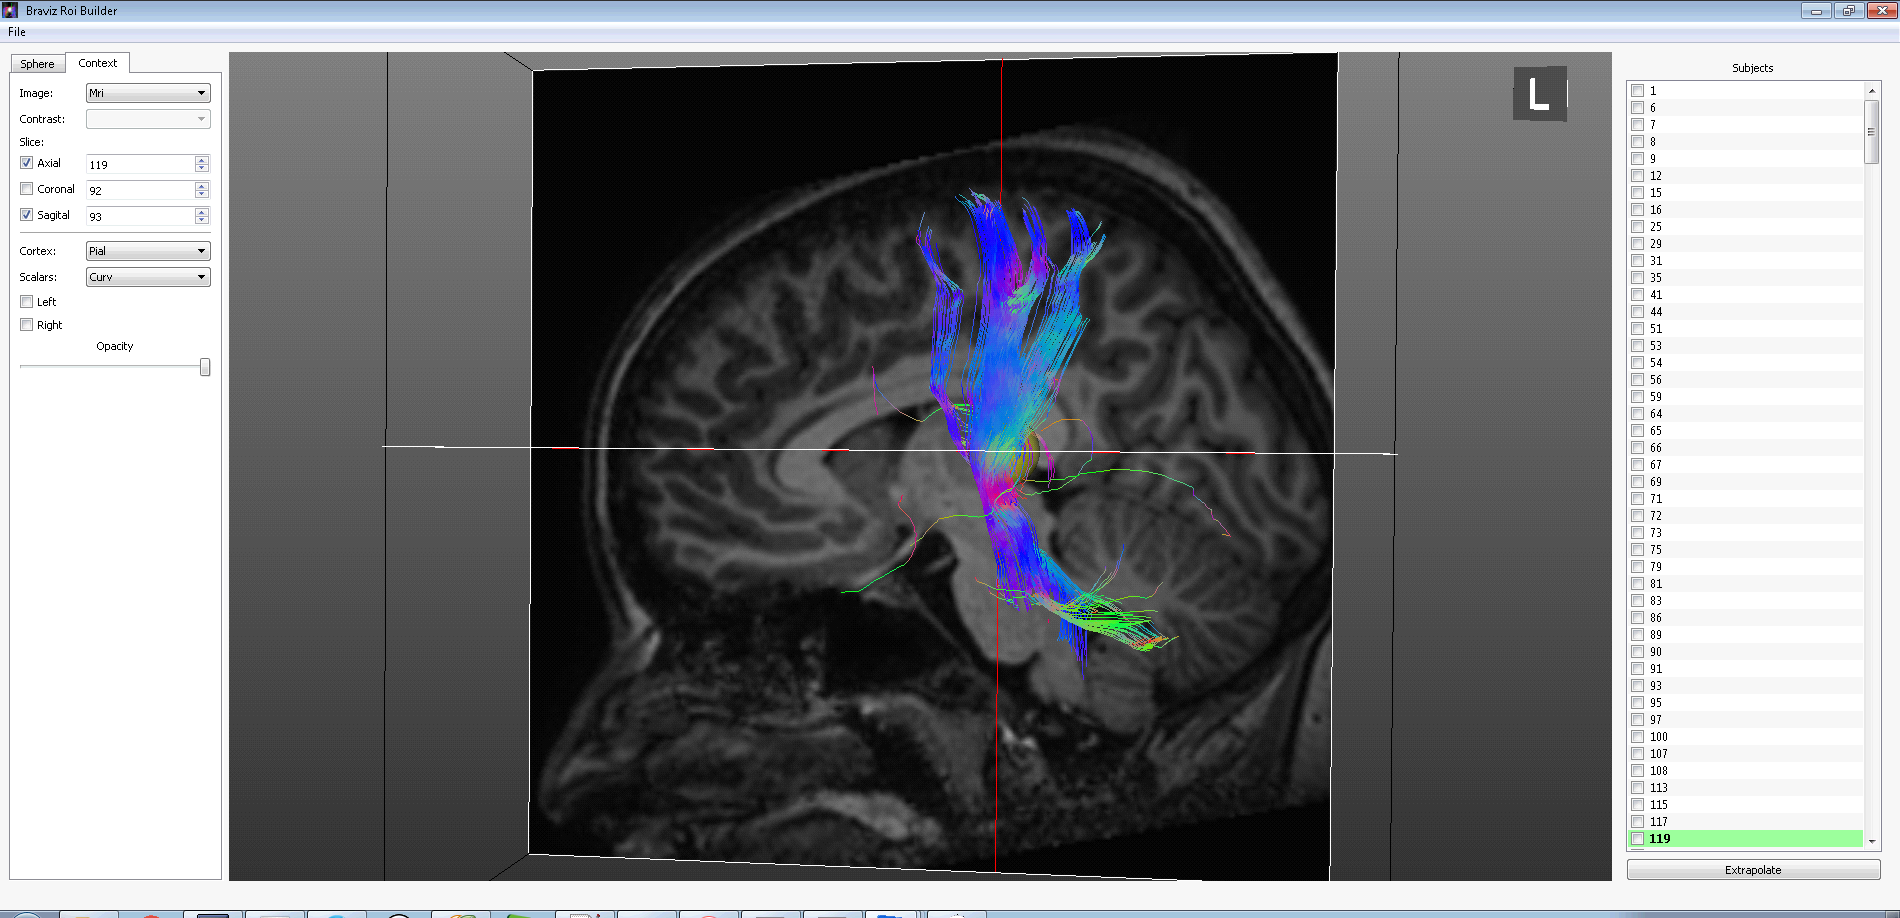
\includegraphics[width=\textwidth, trim = 450pt 150pt 400pt 100pt, clip]{kmc400/thalamus_side_fibers}
		\caption{}
	\end{subfigure}
	\begin{subfigure}{0.45\textwidth}
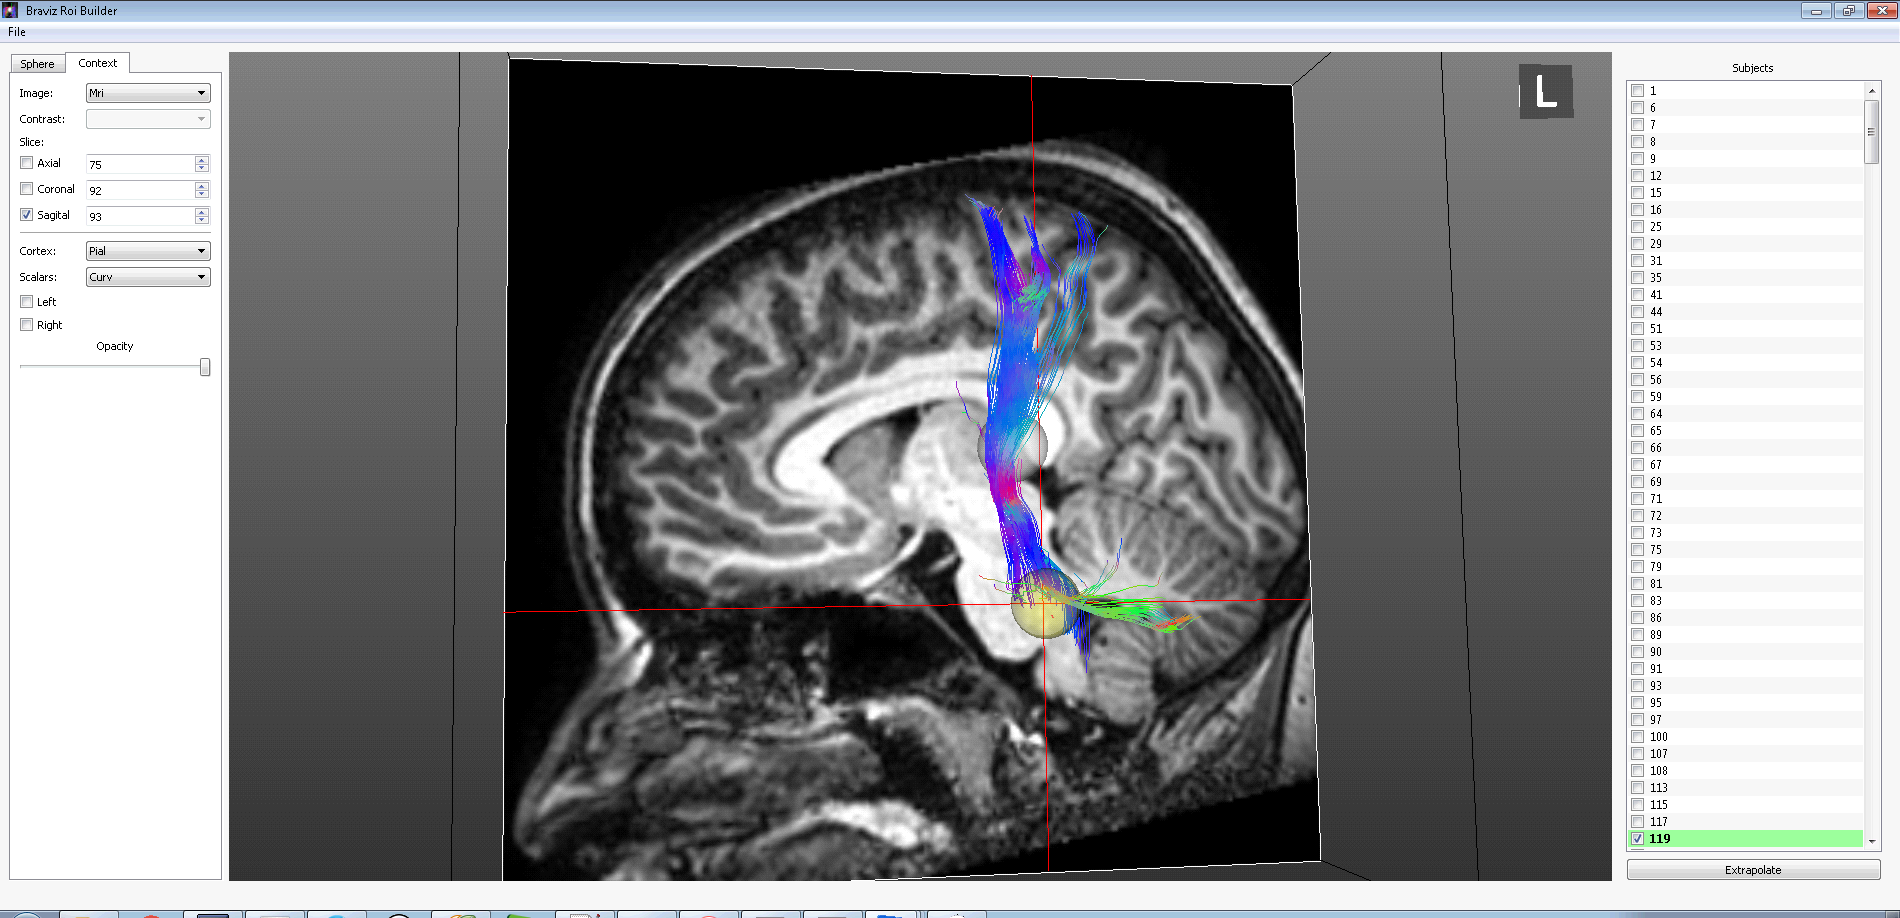
\includegraphics[width=\textwidth, trim = 450pt 150pt 400pt 100pt, clip]{kmc400/thalamus_side_fibers_peduncle}
		\caption{}
	\end{subfigure}
\caption{Combining two ROIs to better isolate a fiber bundle
\label{fig_thalamus_fibers}}
\end{figure}



Figure \ref{fig_fronto_occipital} shows how the fronto occipital tract can be isolated using two spherical ROIs. This tract is a long association way  important for visual memory. Two different subjects are shown, with different number of fibers on this tract. Both of them were born at 28 weeks of gestation and with weights close to 950 grams; however the one with the less dense tracts suffers from a neuro-sensorial alteration.

\begin{figure}
\centering
	\begin{subfigure}{0.45\textwidth}
		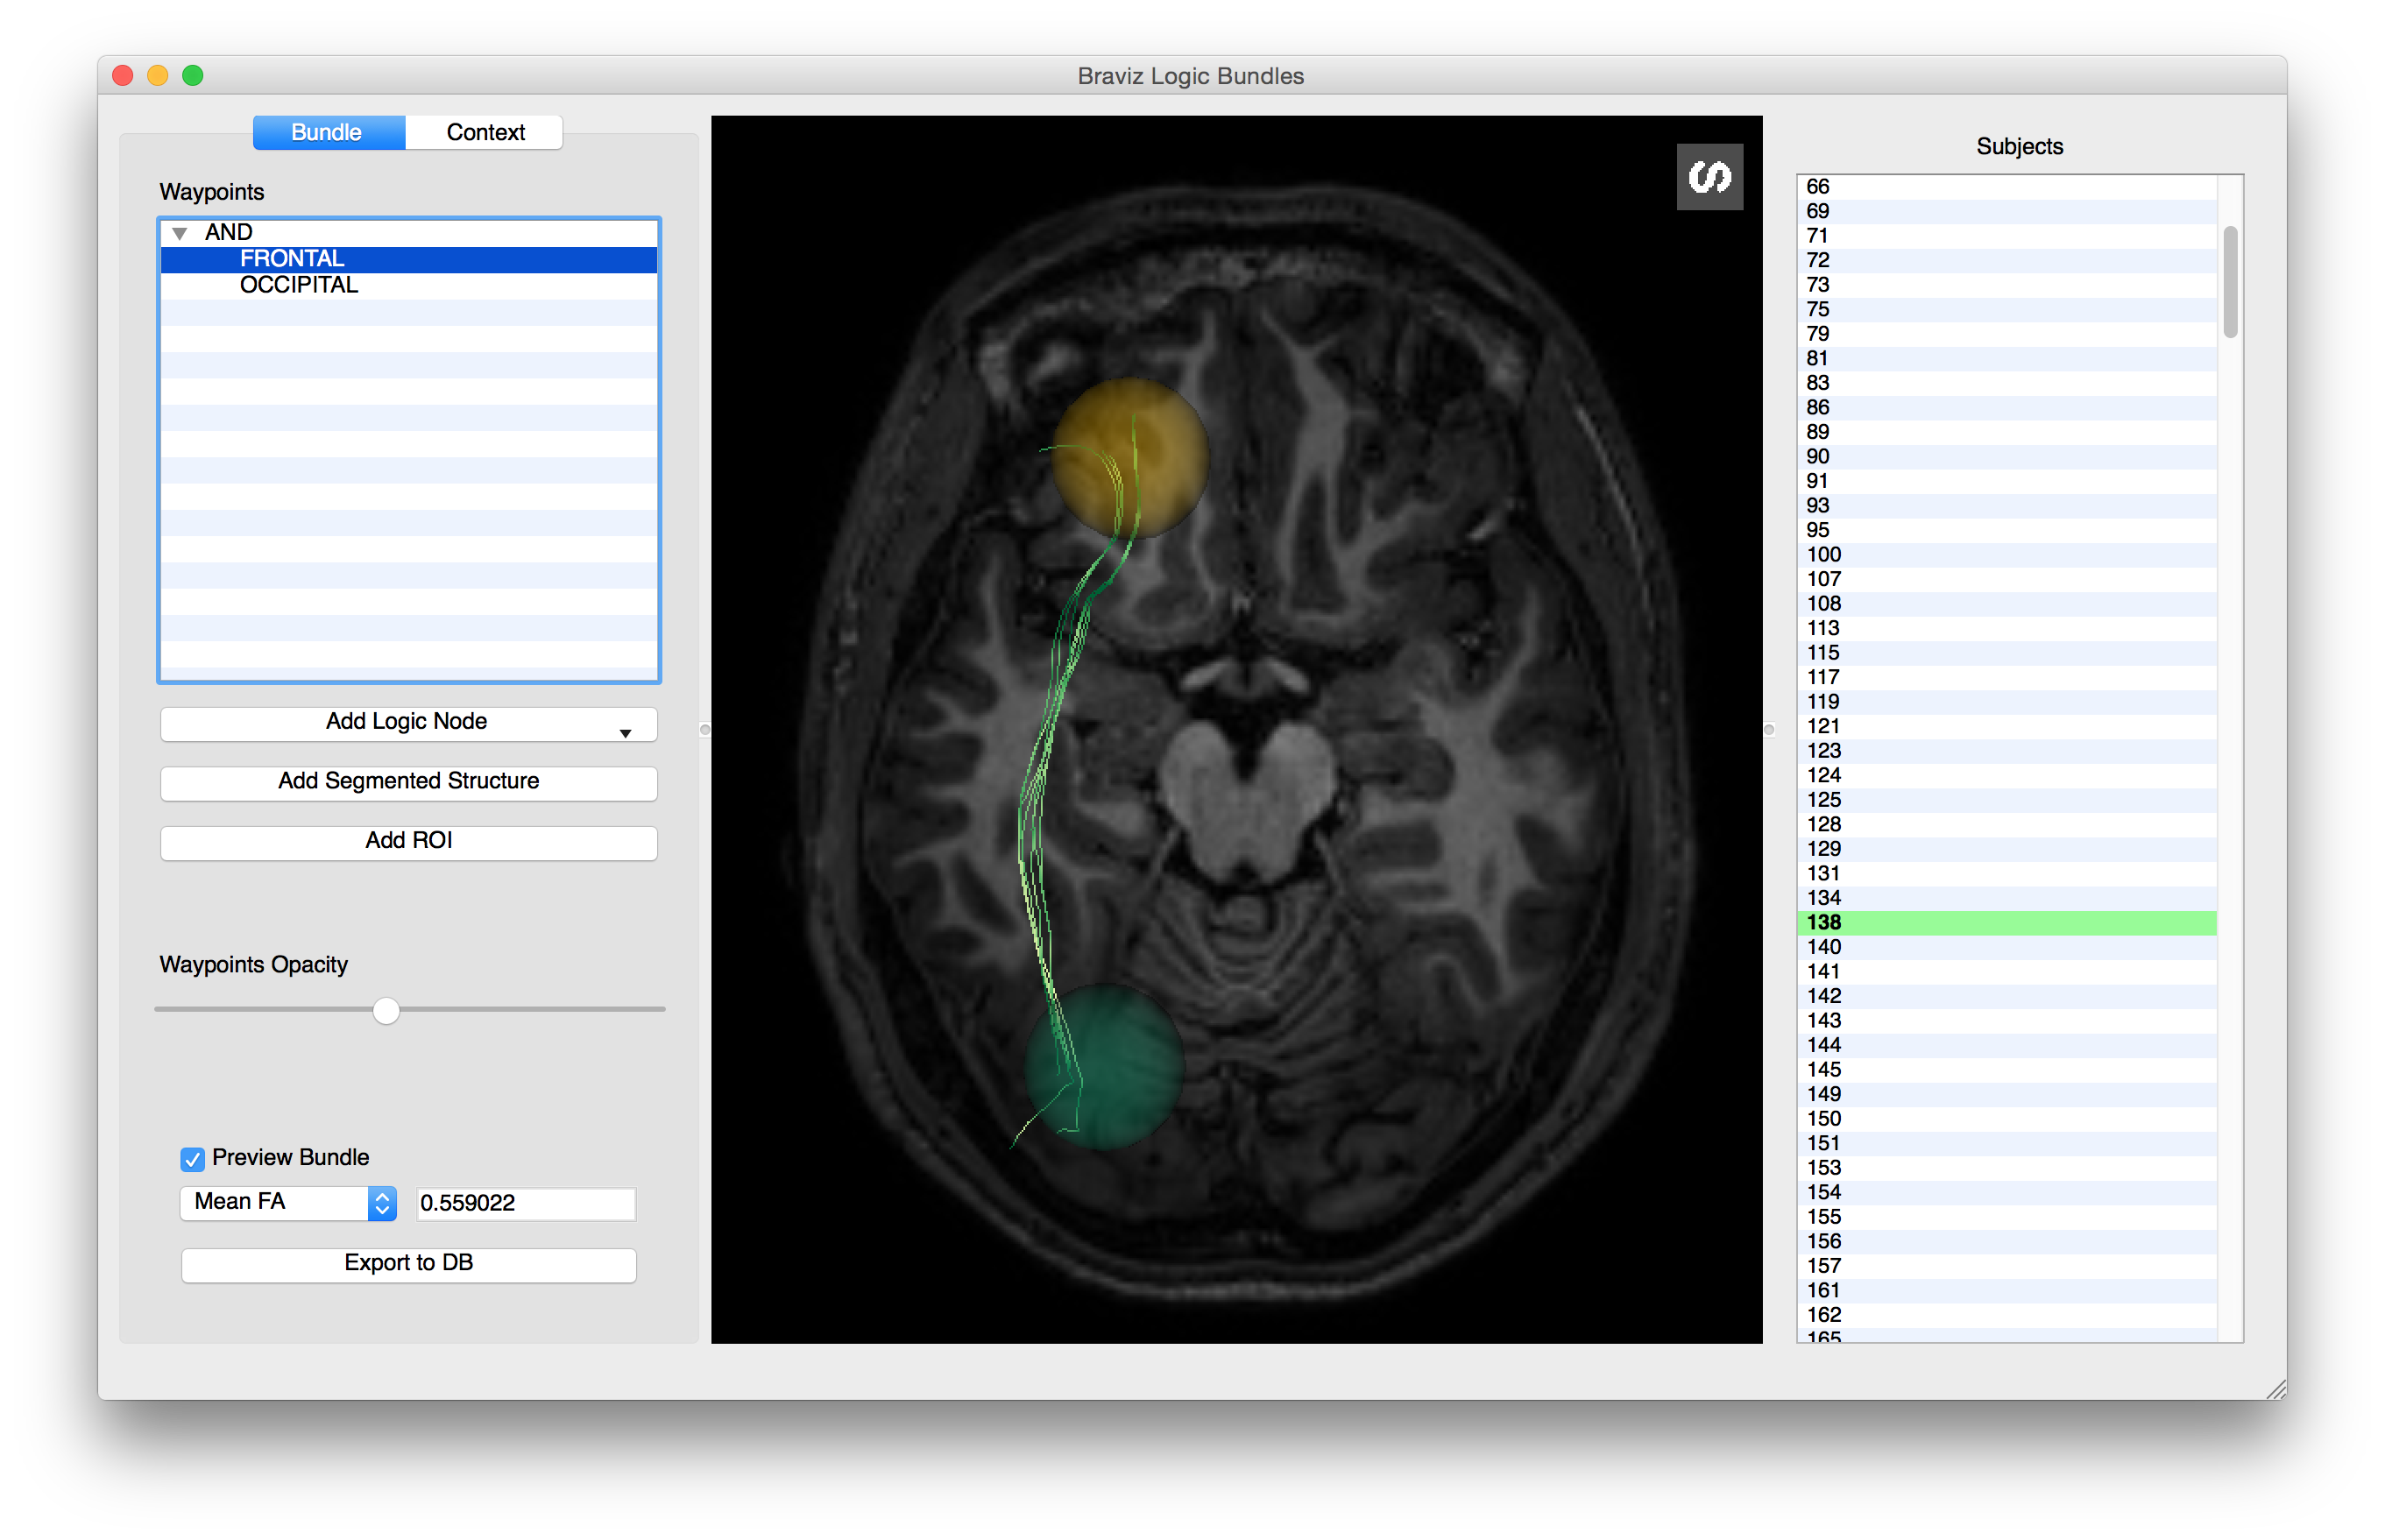
\includegraphics[width=\textwidth, trim = 450pt 150pt 400pt 100pt, clip]{kmc400/fronto_occipital_1}
		\caption{}
	\end{subfigure}
	\begin{subfigure}{0.45\textwidth}
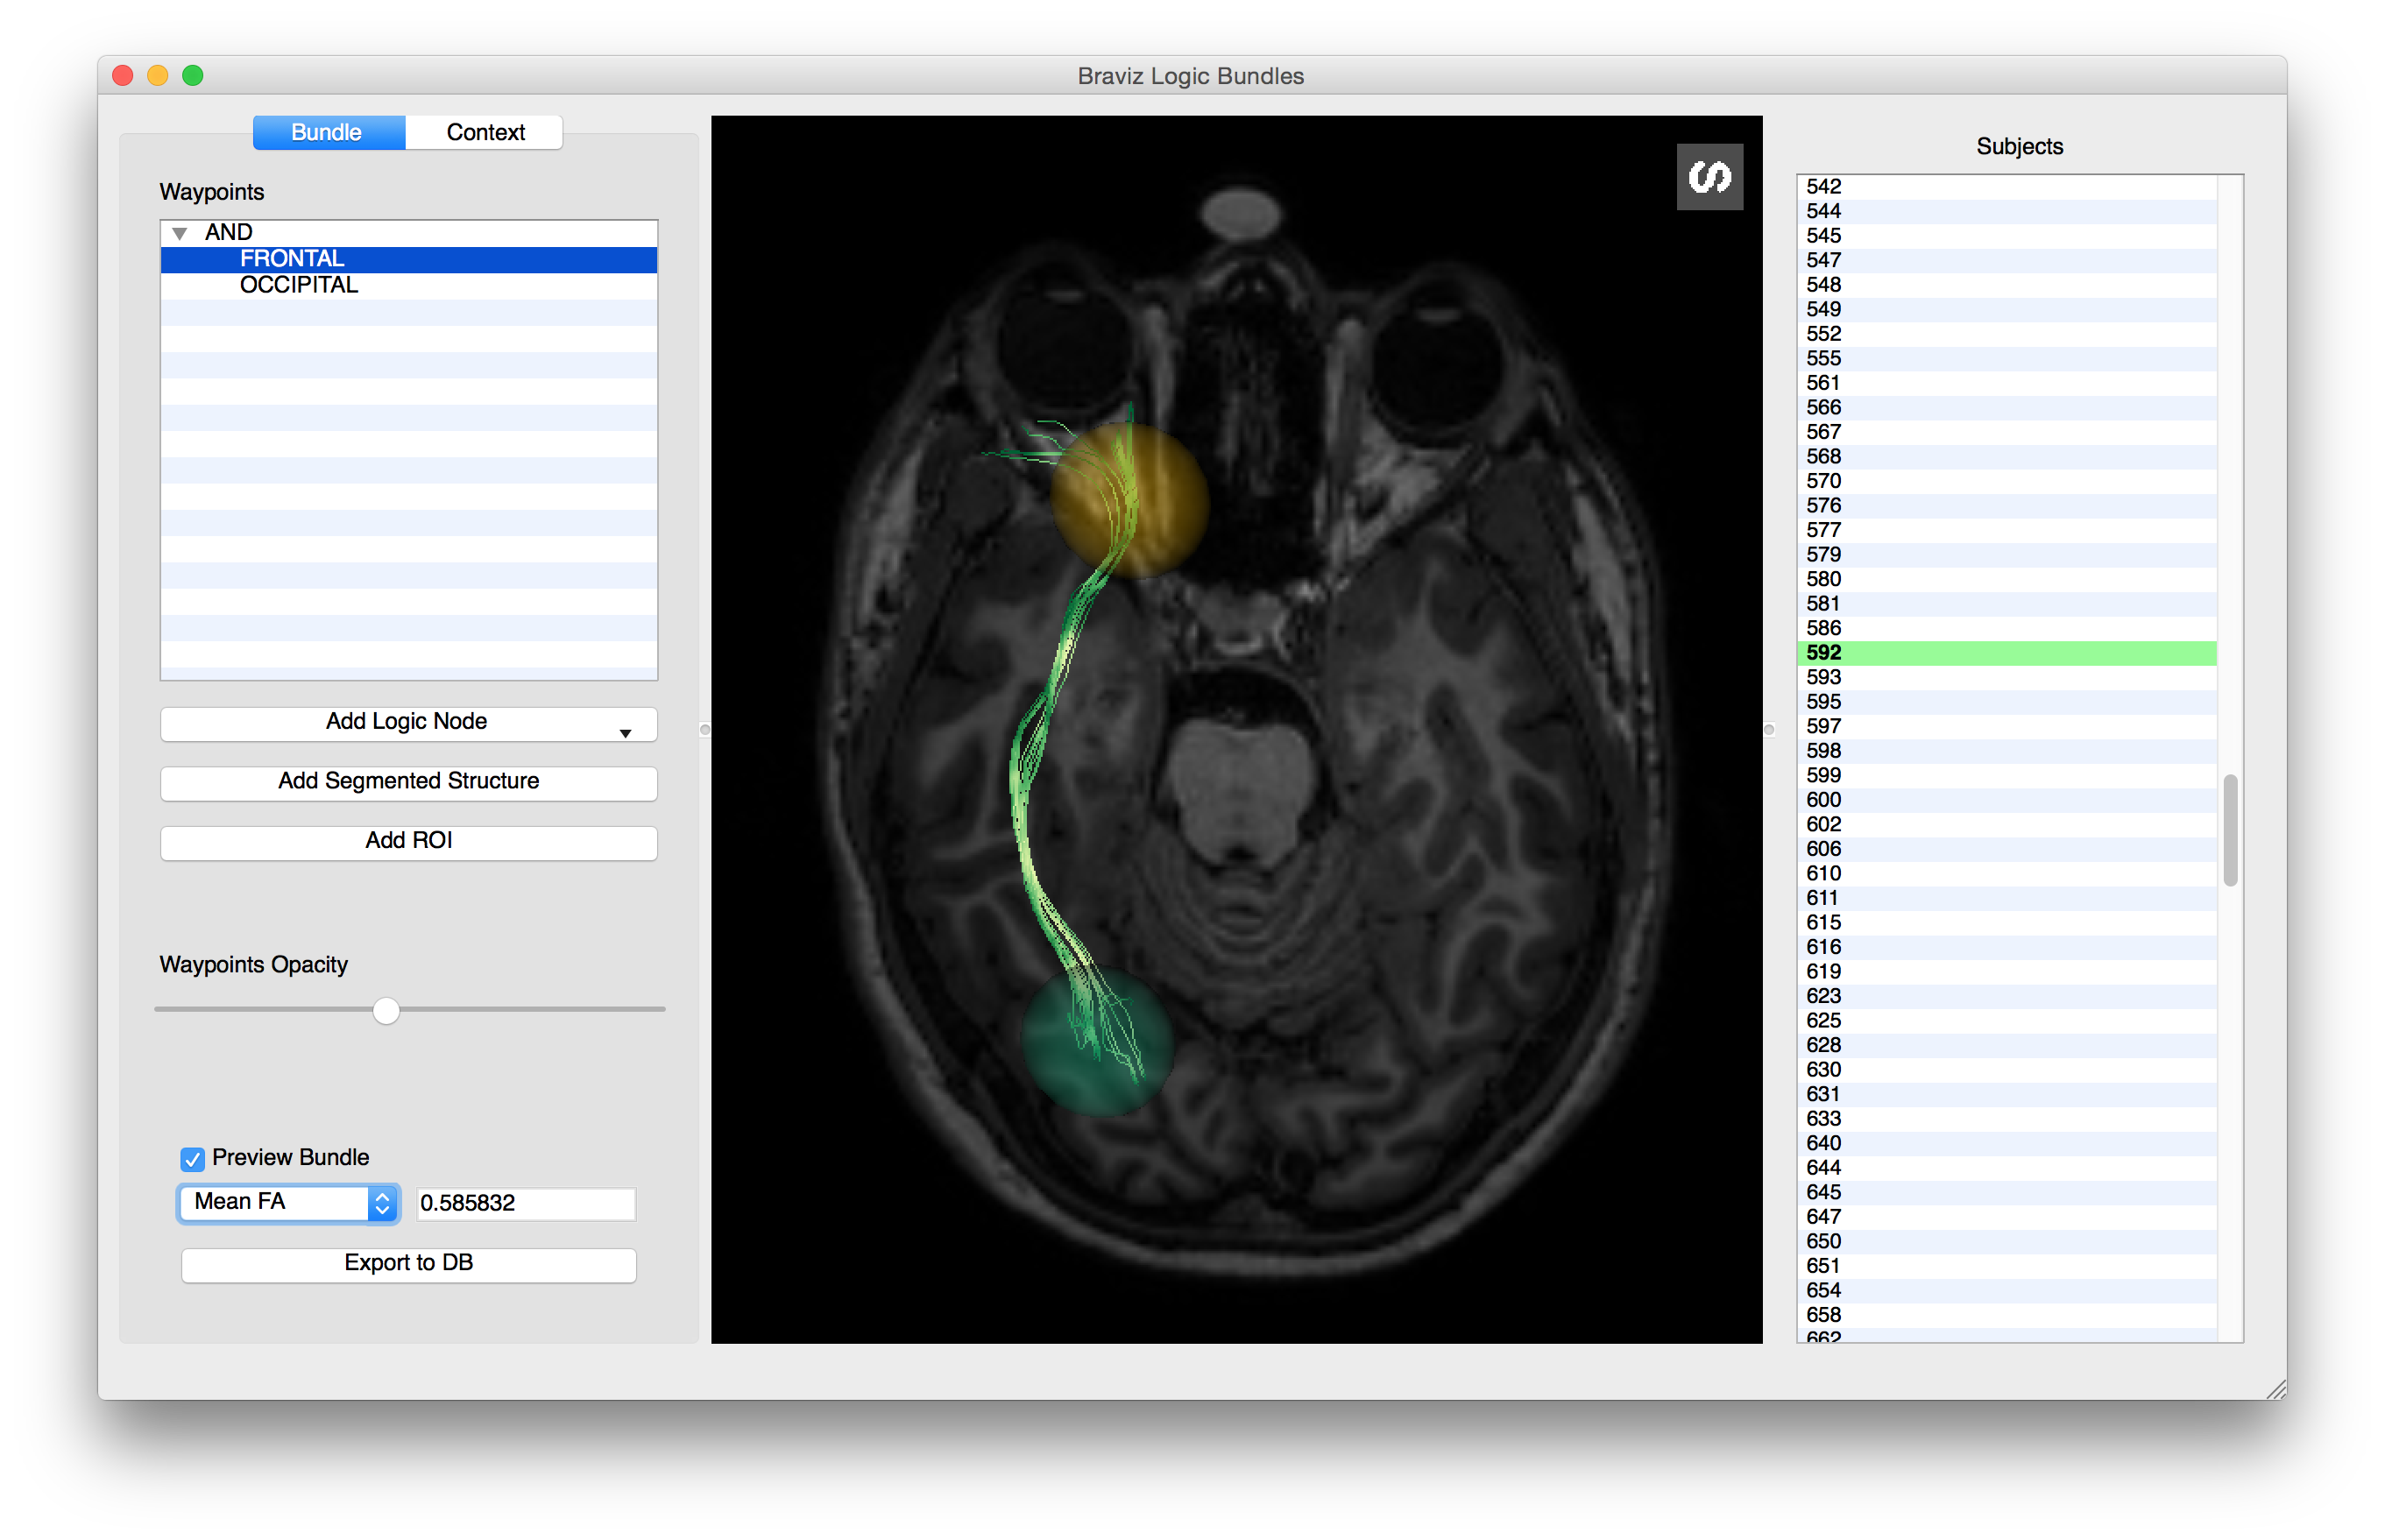
\includegraphics[width=\textwidth, trim = 450pt 150pt 400pt 100pt, clip]{kmc400/fronto_occipital_2}
		\caption{}
	\end{subfigure}
\caption{Isolation of the fronto occipital tracts using two ROIs, the subject in (a) suffers from a neuro-sensorial alteration
\label{fig_fronto_occipital}}
\end{figure}


The superior longitudinal fasciculus can be isolated by placing a single ROI in the coronal plane. Figure \ref{fig_long_fasc} shows the result of this operation and a comparison to the equivalent bundle identified by Tracula. 

\begin{figure}
\centering
	\begin{subfigure}{0.45\textwidth}
		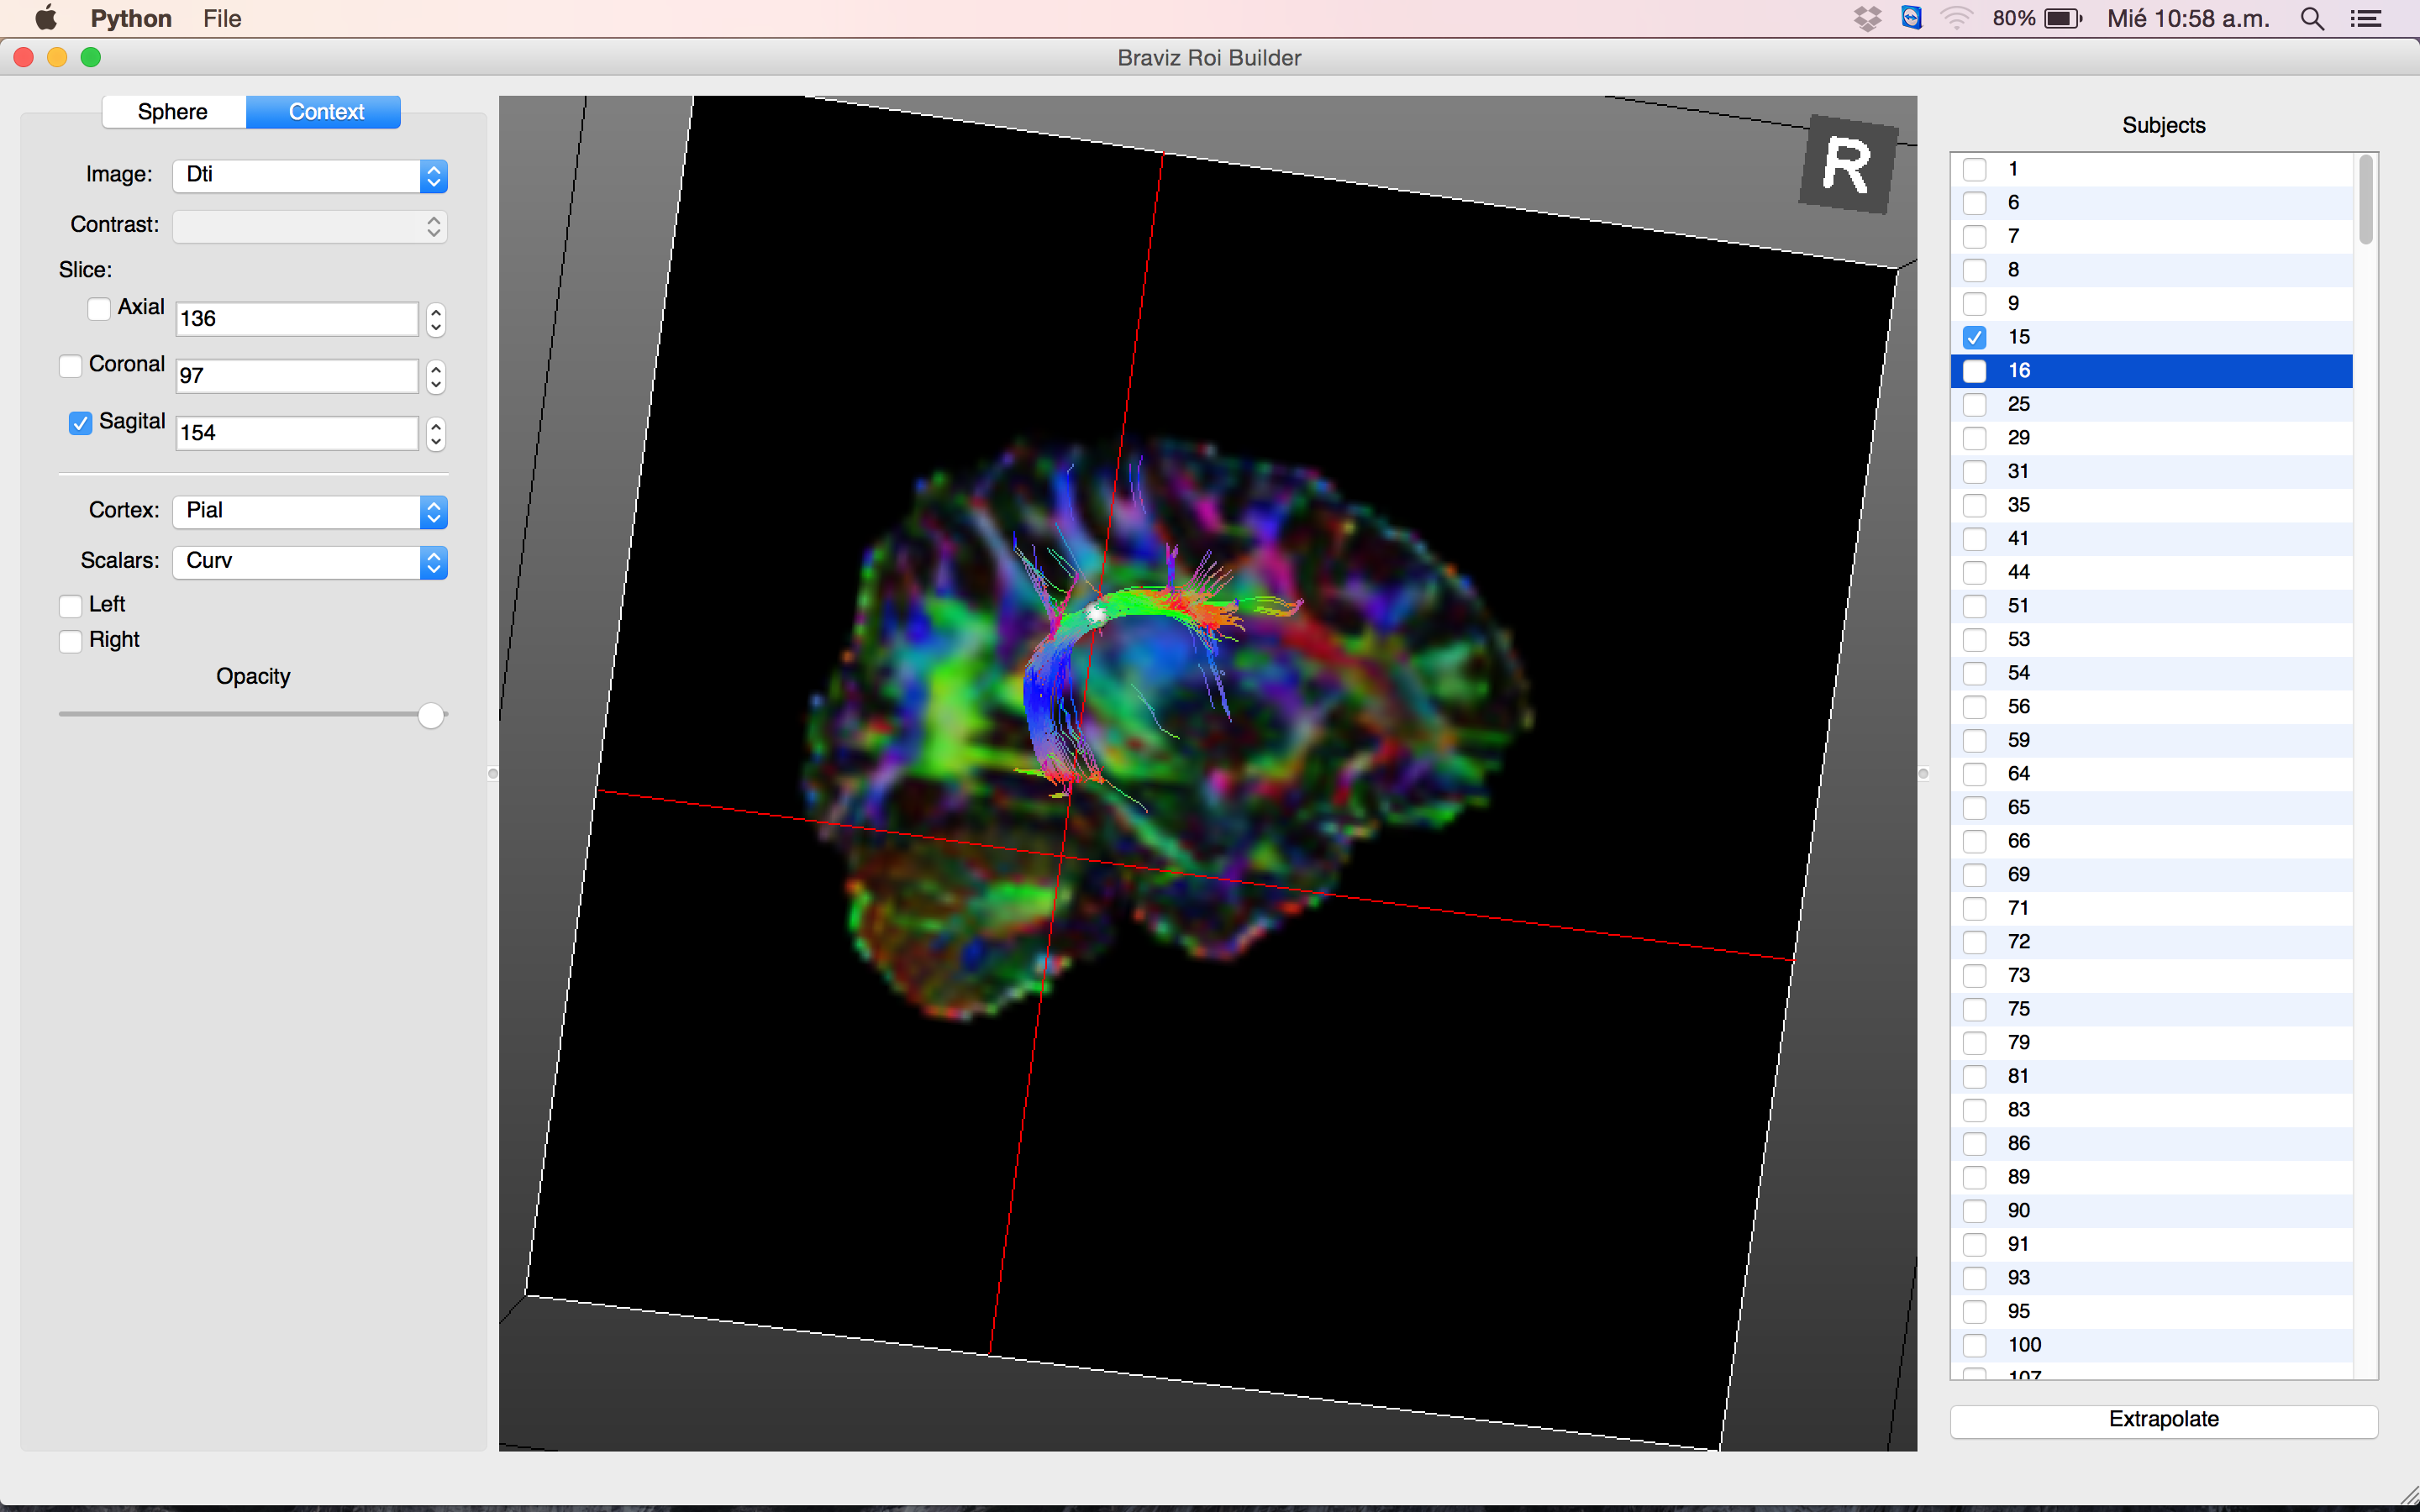
\includegraphics[width=\textwidth, trim=300pt 250pt 350pt 250pt, clip]{kmc400/long_coronal_seed}
		\caption{ROI placement}
	\end{subfigure}
	\begin{subfigure}{0.45\textwidth}
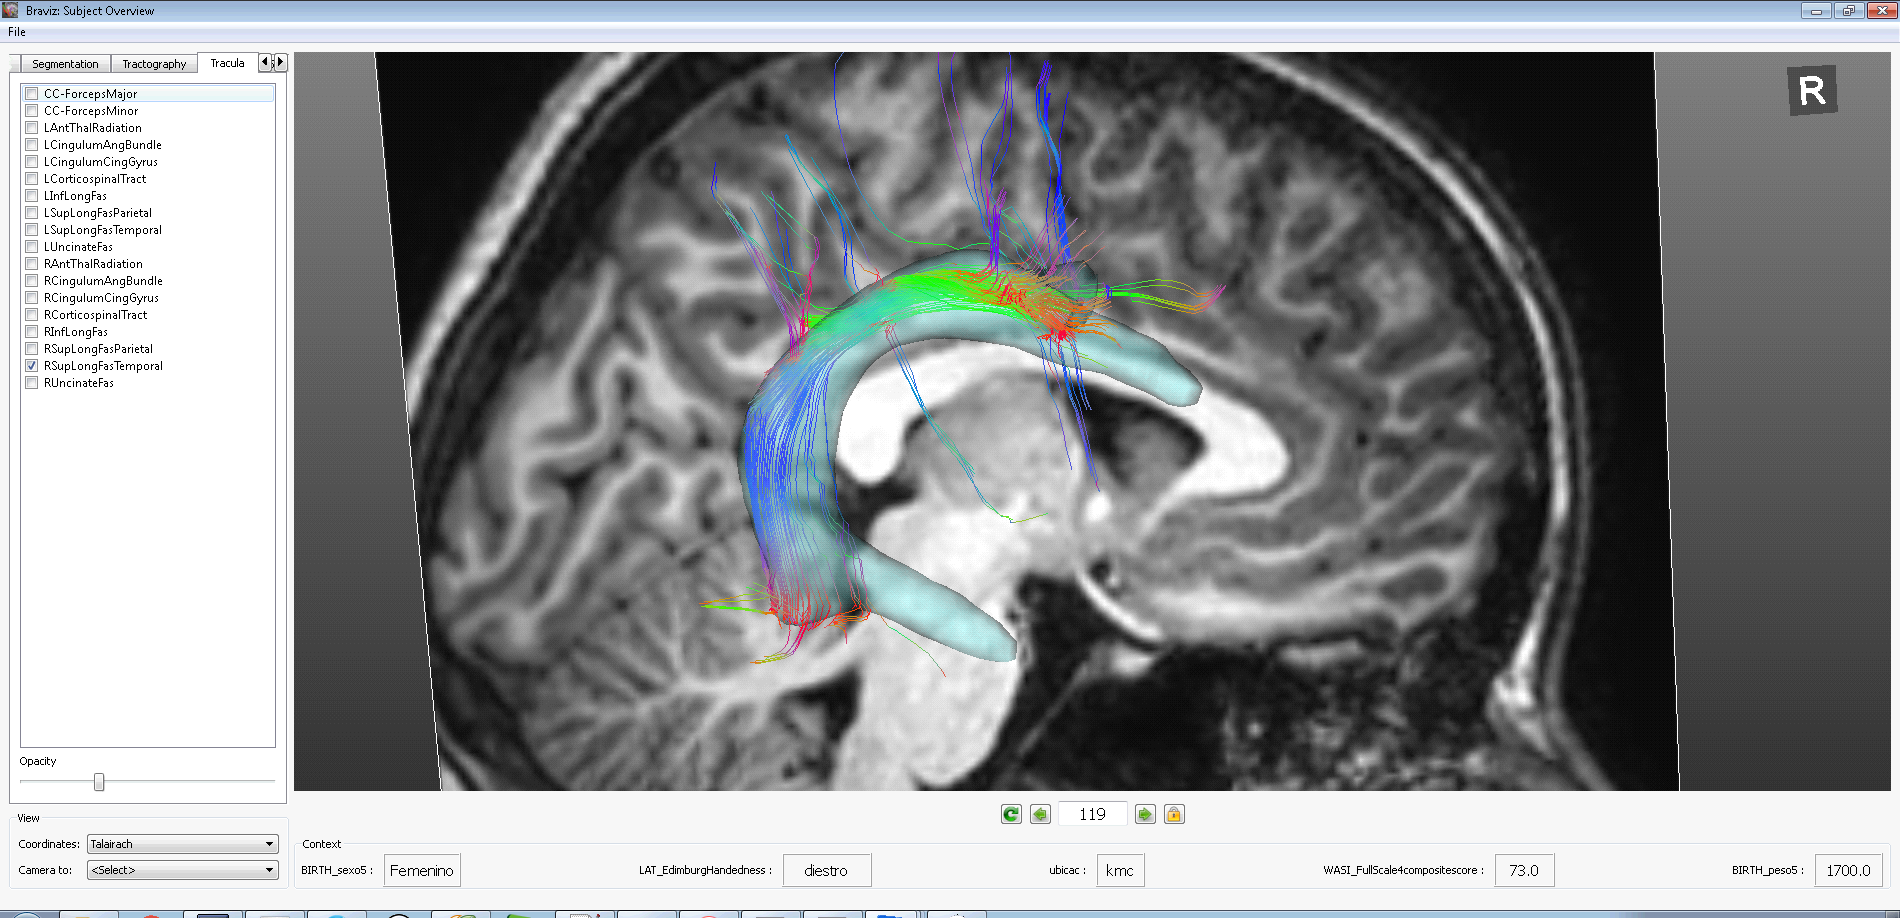
\includegraphics[width=\textwidth, trim = 250pt 100pt 50pt 20pt, clip]{kmc400/long_fas_tracula_roi}
		\caption{Comparison with Tracula}
	\end{subfigure}

\caption{Reconstruction of the longitudinal fasciculus using a region of interest.
\label{fig_long_fasc}}
\end{figure} 

After positioning the spherical region on one subject, the application can approximate the equivalent location for the rest of the sample by using the available linear and non linear registration transforms. These locations would then be revised and adjusted by the expert, but the interface was built to make this process as efficient as possible. All actions can be completed using hot-keys, including changing subjects, therefore the user interactions are limited to moving the mouse around a small area and hitting keys on the keyboard.

ROIs can also be used to measure FA, MD, T-score from a functional paradigm or any the value of any other image inside it. This was used in the study to measure diffusion characteristics at several points of interest, which are known to be at risk in preterm babies. These points were

\begin{itemize}
\item Optic Chiasm
\item Optic tract back of the chiasm at both sides
\item Corona radiata
\item Left and right tapetum
\item Left and right lateral geniculate nuclei
\item Posterior Thalamus
\end{itemize}

These values were used in statistical analyses throughout the study, both inside Braviz itself, and exported to the main SPSS database.

The \emph{Logic Bundles} application can be used to define bundles using segmented structures and ROIs as waypoints. Figure \ref{fig_papez} shows the fibers between the amygdala and the hippocampus, which is part of the Papez circuit. 

\begin{figure}
\centering
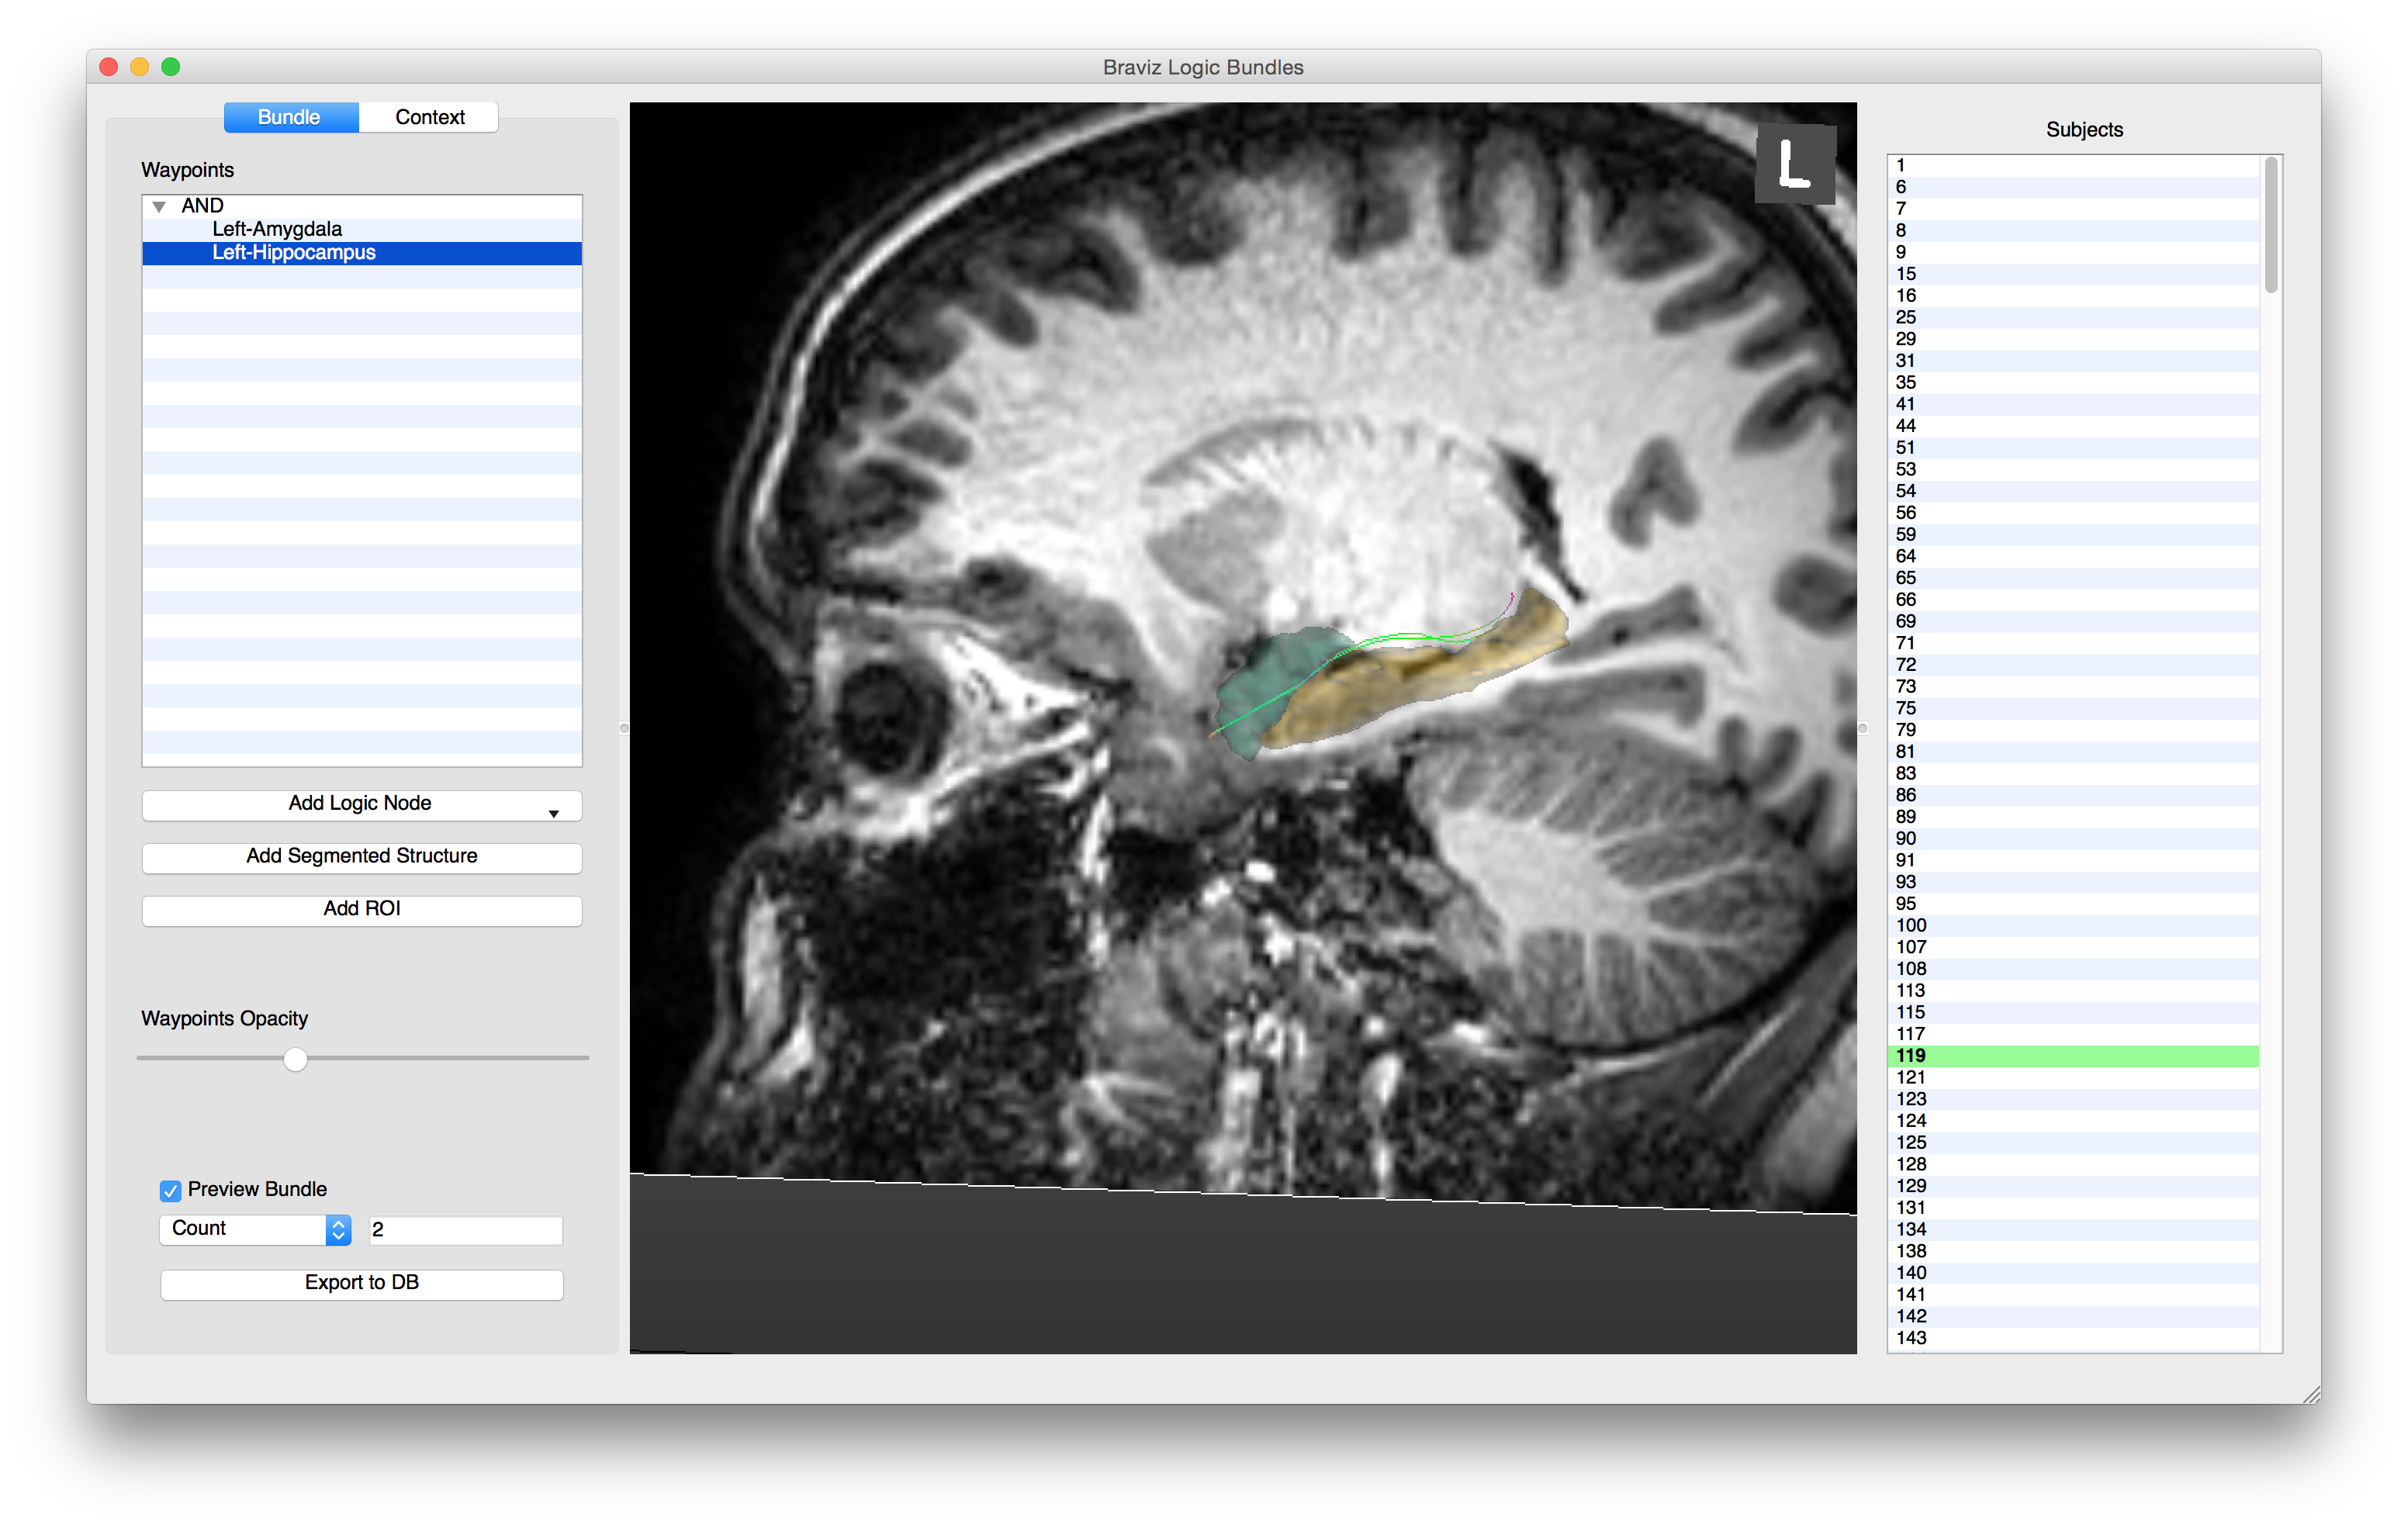
\includegraphics[width=0.5\textwidth, clip, trim = 450pt 200pt 350pt 80pt]{kmc400/papez}
\caption{Using logic bundles to isolate the fibers that go through the amygdala and the hypothalamus
\label{fig_papez}}
\end{figure} 



%sharing, presentations

\subsubsection{Data exploration}

One of the main purposes of Braviz was enabling researchers to quickly find potential relationships in the data that deserved a closer look. Displaying data visually lets the human visual system find odd aspects, which can lead experts to think of new possibilities. 

Figure \ref{fig_anova_example} shows the plot of an ANOVA analysis for the volume of the left caudate nucleus against the exposure variable and a fragility index. The plot shows that the most fragile subjects tend to have smaller caudate nuclei in both groups, but this relationship is not statisticially significant. Nevertheless it is worth taking a closer look and analyze if there is a biological justification for it. If this is the case, maybe it is worth collecting more data in order to test this new hypothesis. Figure \ref{fig_caudate_parallel} shows another view of this relationship, this time showing left and right caudate nuclei. From the plot it can be seen that for most subjects both nuclei tend to have the same volume, and these are negatively related to the fragility index. It also calls attention an outlier who has a strong asymmetry. Figure \ref{fig_asymetric_caudate_detail} shows this outlier on the \emph{Subject Overview} application; where it can be confirmed that the asymmetry is real. This can be seen directly on the image as well as on the notes written by the radiologist.


\begin{figure}
	\centering
		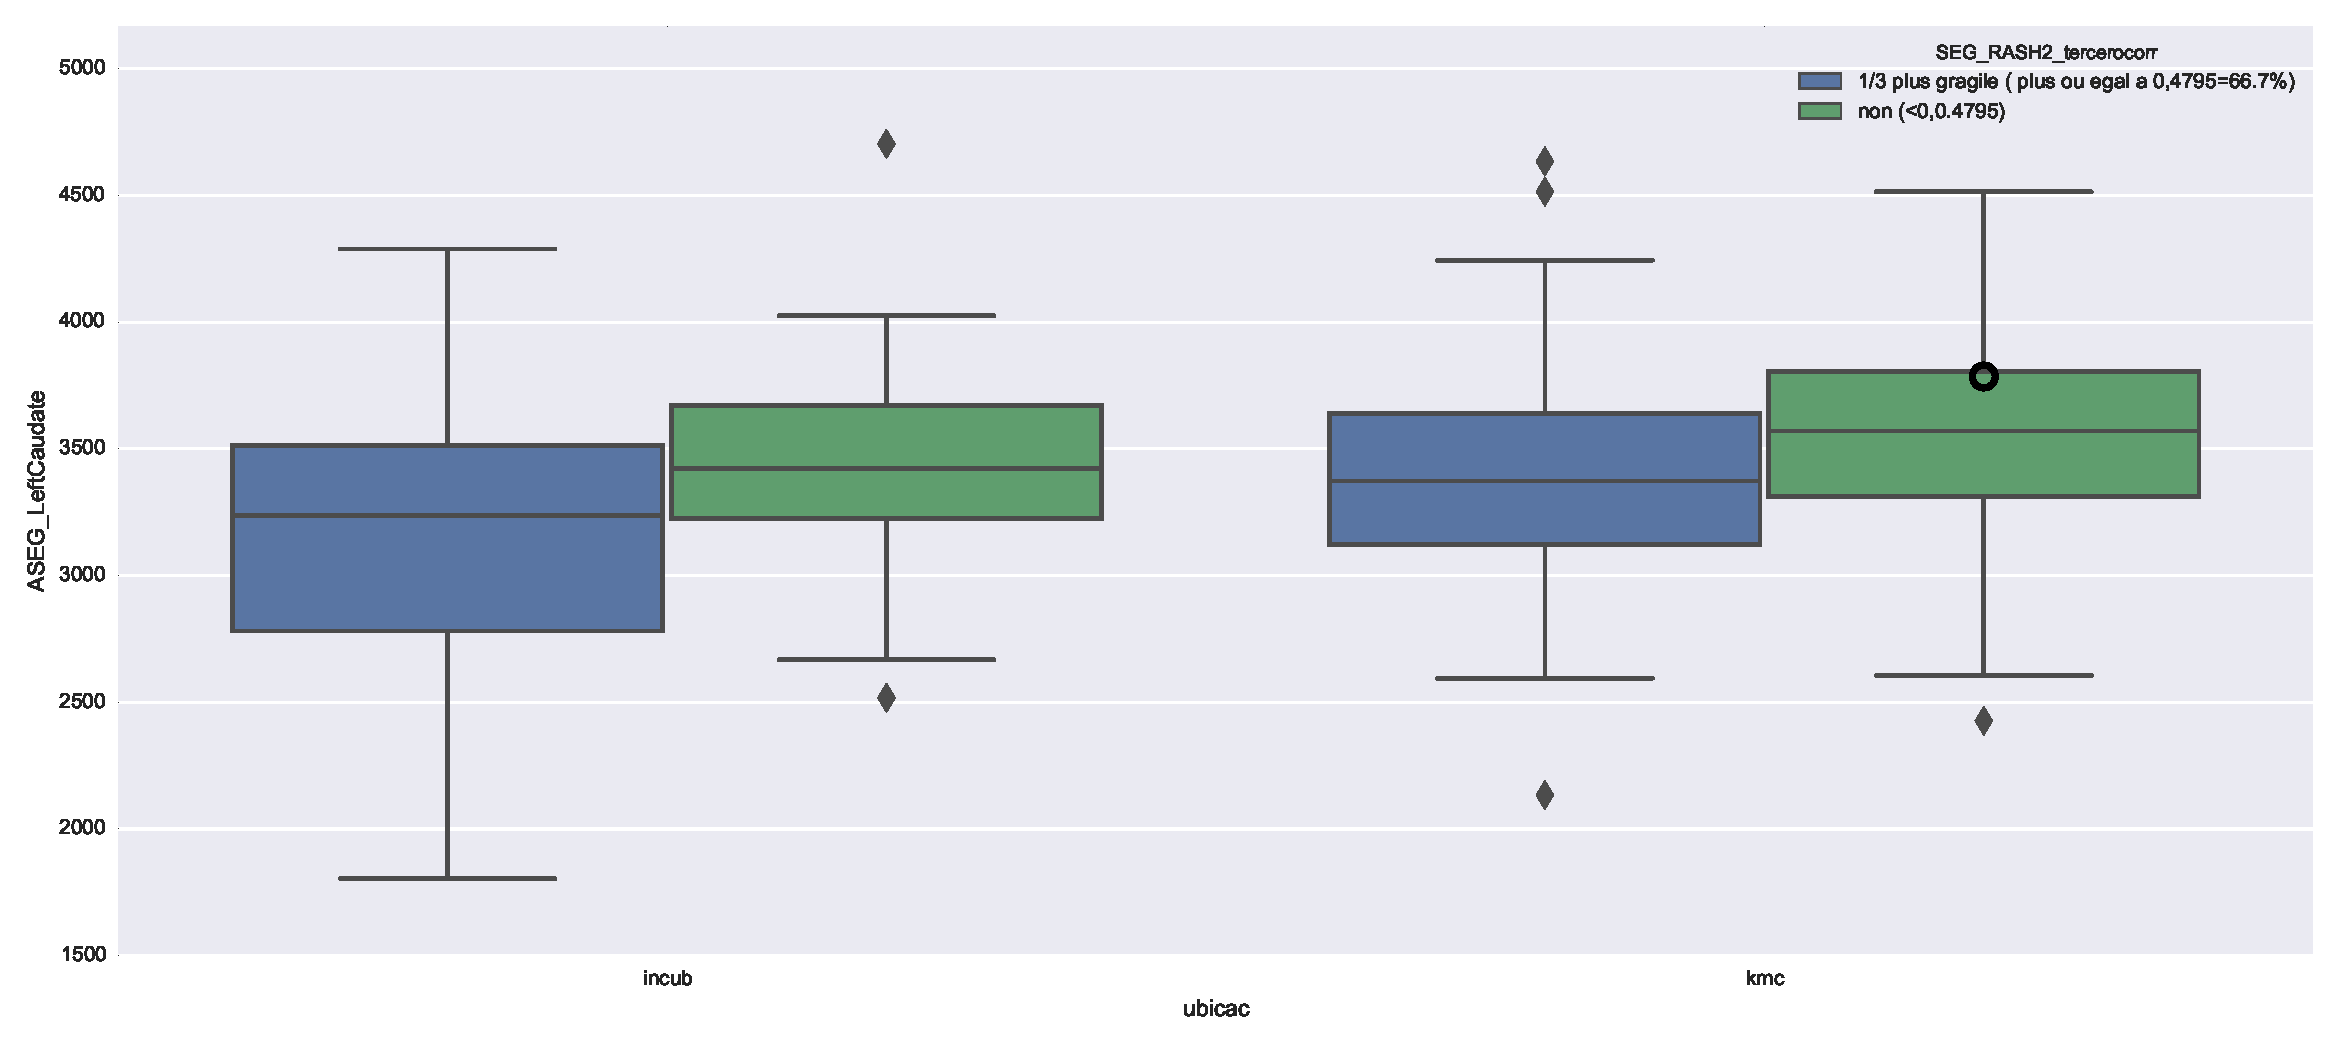
\includegraphics[width=\textwidth]{figures/kmc400/left_caudate_fragility_anova}
	\caption{An anova analysis of the volume of the left caudate nucleus against a fragility index and the treatment variable}
	\label{fig_anova_example}
\end{figure}


\begin{figure}
	\centering
		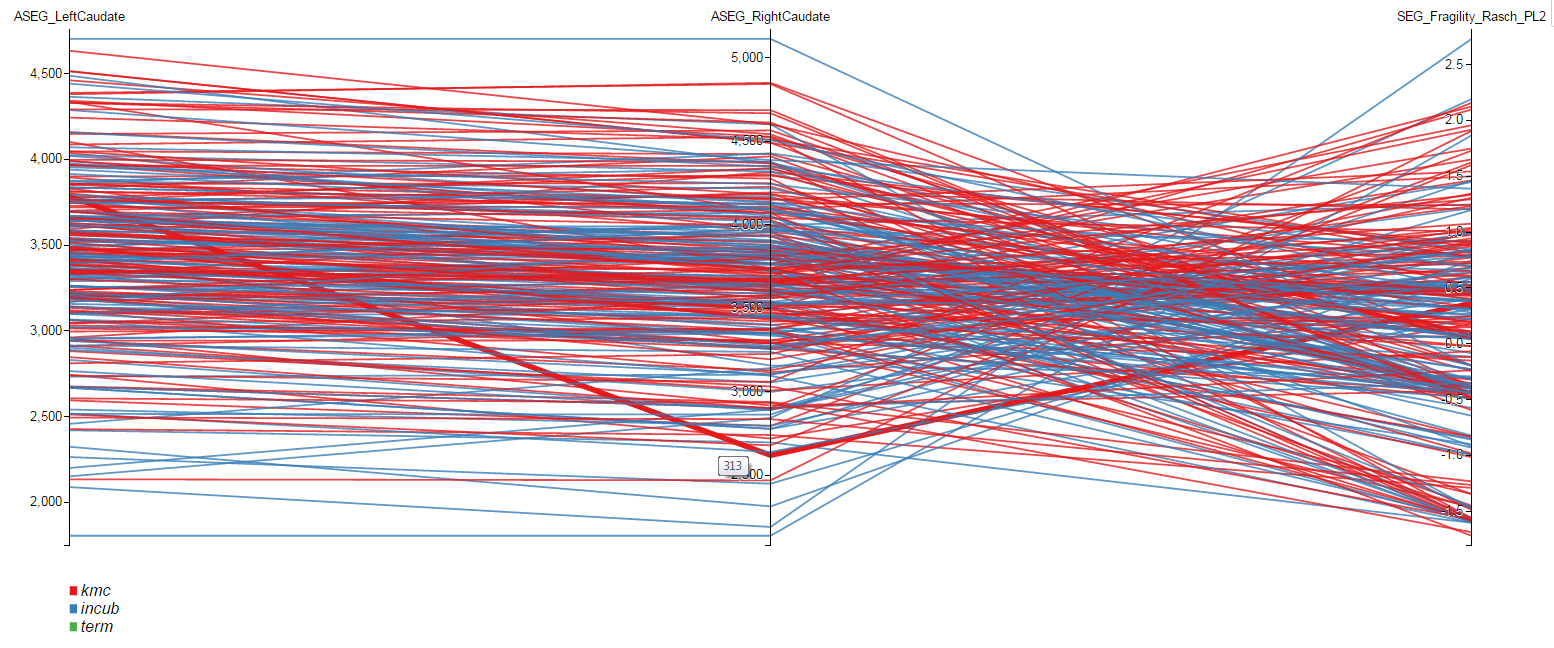
\includegraphics[width=\textwidth]{figures/kmc400/caudate_parallel}
	\caption{A parallel coordinates view of the left and right caudates in relationship with the fragility index. There is a clear negative correlation between the volumes of these structures and the fragility index, and a clear outlier.}
	\label{fig_caudate_parallel}
\end{figure}


\begin{figure}
	\centering
		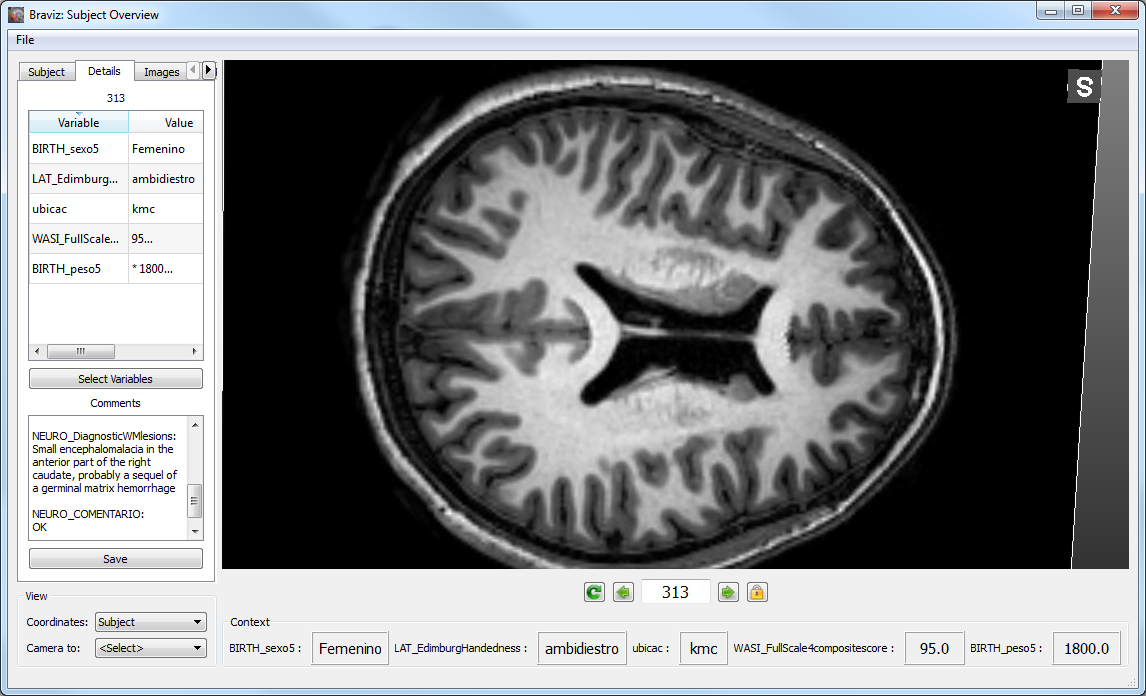
\includegraphics[width=\textwidth]{kmc400/caudate_detail}
	\caption{Detailed view of the outlier from figure \ref{fig_caudate_parallel}, it confirms that the strange behavior exhibited is real and not a problem with the data.}
	\label{fig_asymetric_caudate_detail}
\end{figure}

\subsubsection{Selected Subjects Cases}
 
% 173
The FLAIR image from one of the subjects present several circular regions with hypersignal which indicate ischemic lesions, this can be seen in Figure \ref{fig_white_matter_lessions_a}. These are typical in patients with sifilis, drug abuse or hypertension, and do not usually appear before birth. The clinical data does not show any drug related problems, but it does  that the subject had a hearing loss which went undetected for the first year of life, and did not improve with by hearing aids or implants. 
The Grifiths coefficient at 12 months had a value of 100 which is located in the middle of the sample, however the WASI coefficient at 20 years old has a value of 69, which is at the lower extreme of the sample (see Figure \ref{fig_white_matter_lessions_b}). This appears to confirm that the lesions occurred after birth.

\begin{figure}
	\centering
	\begin{subfigure}{0.45\textwidth}
		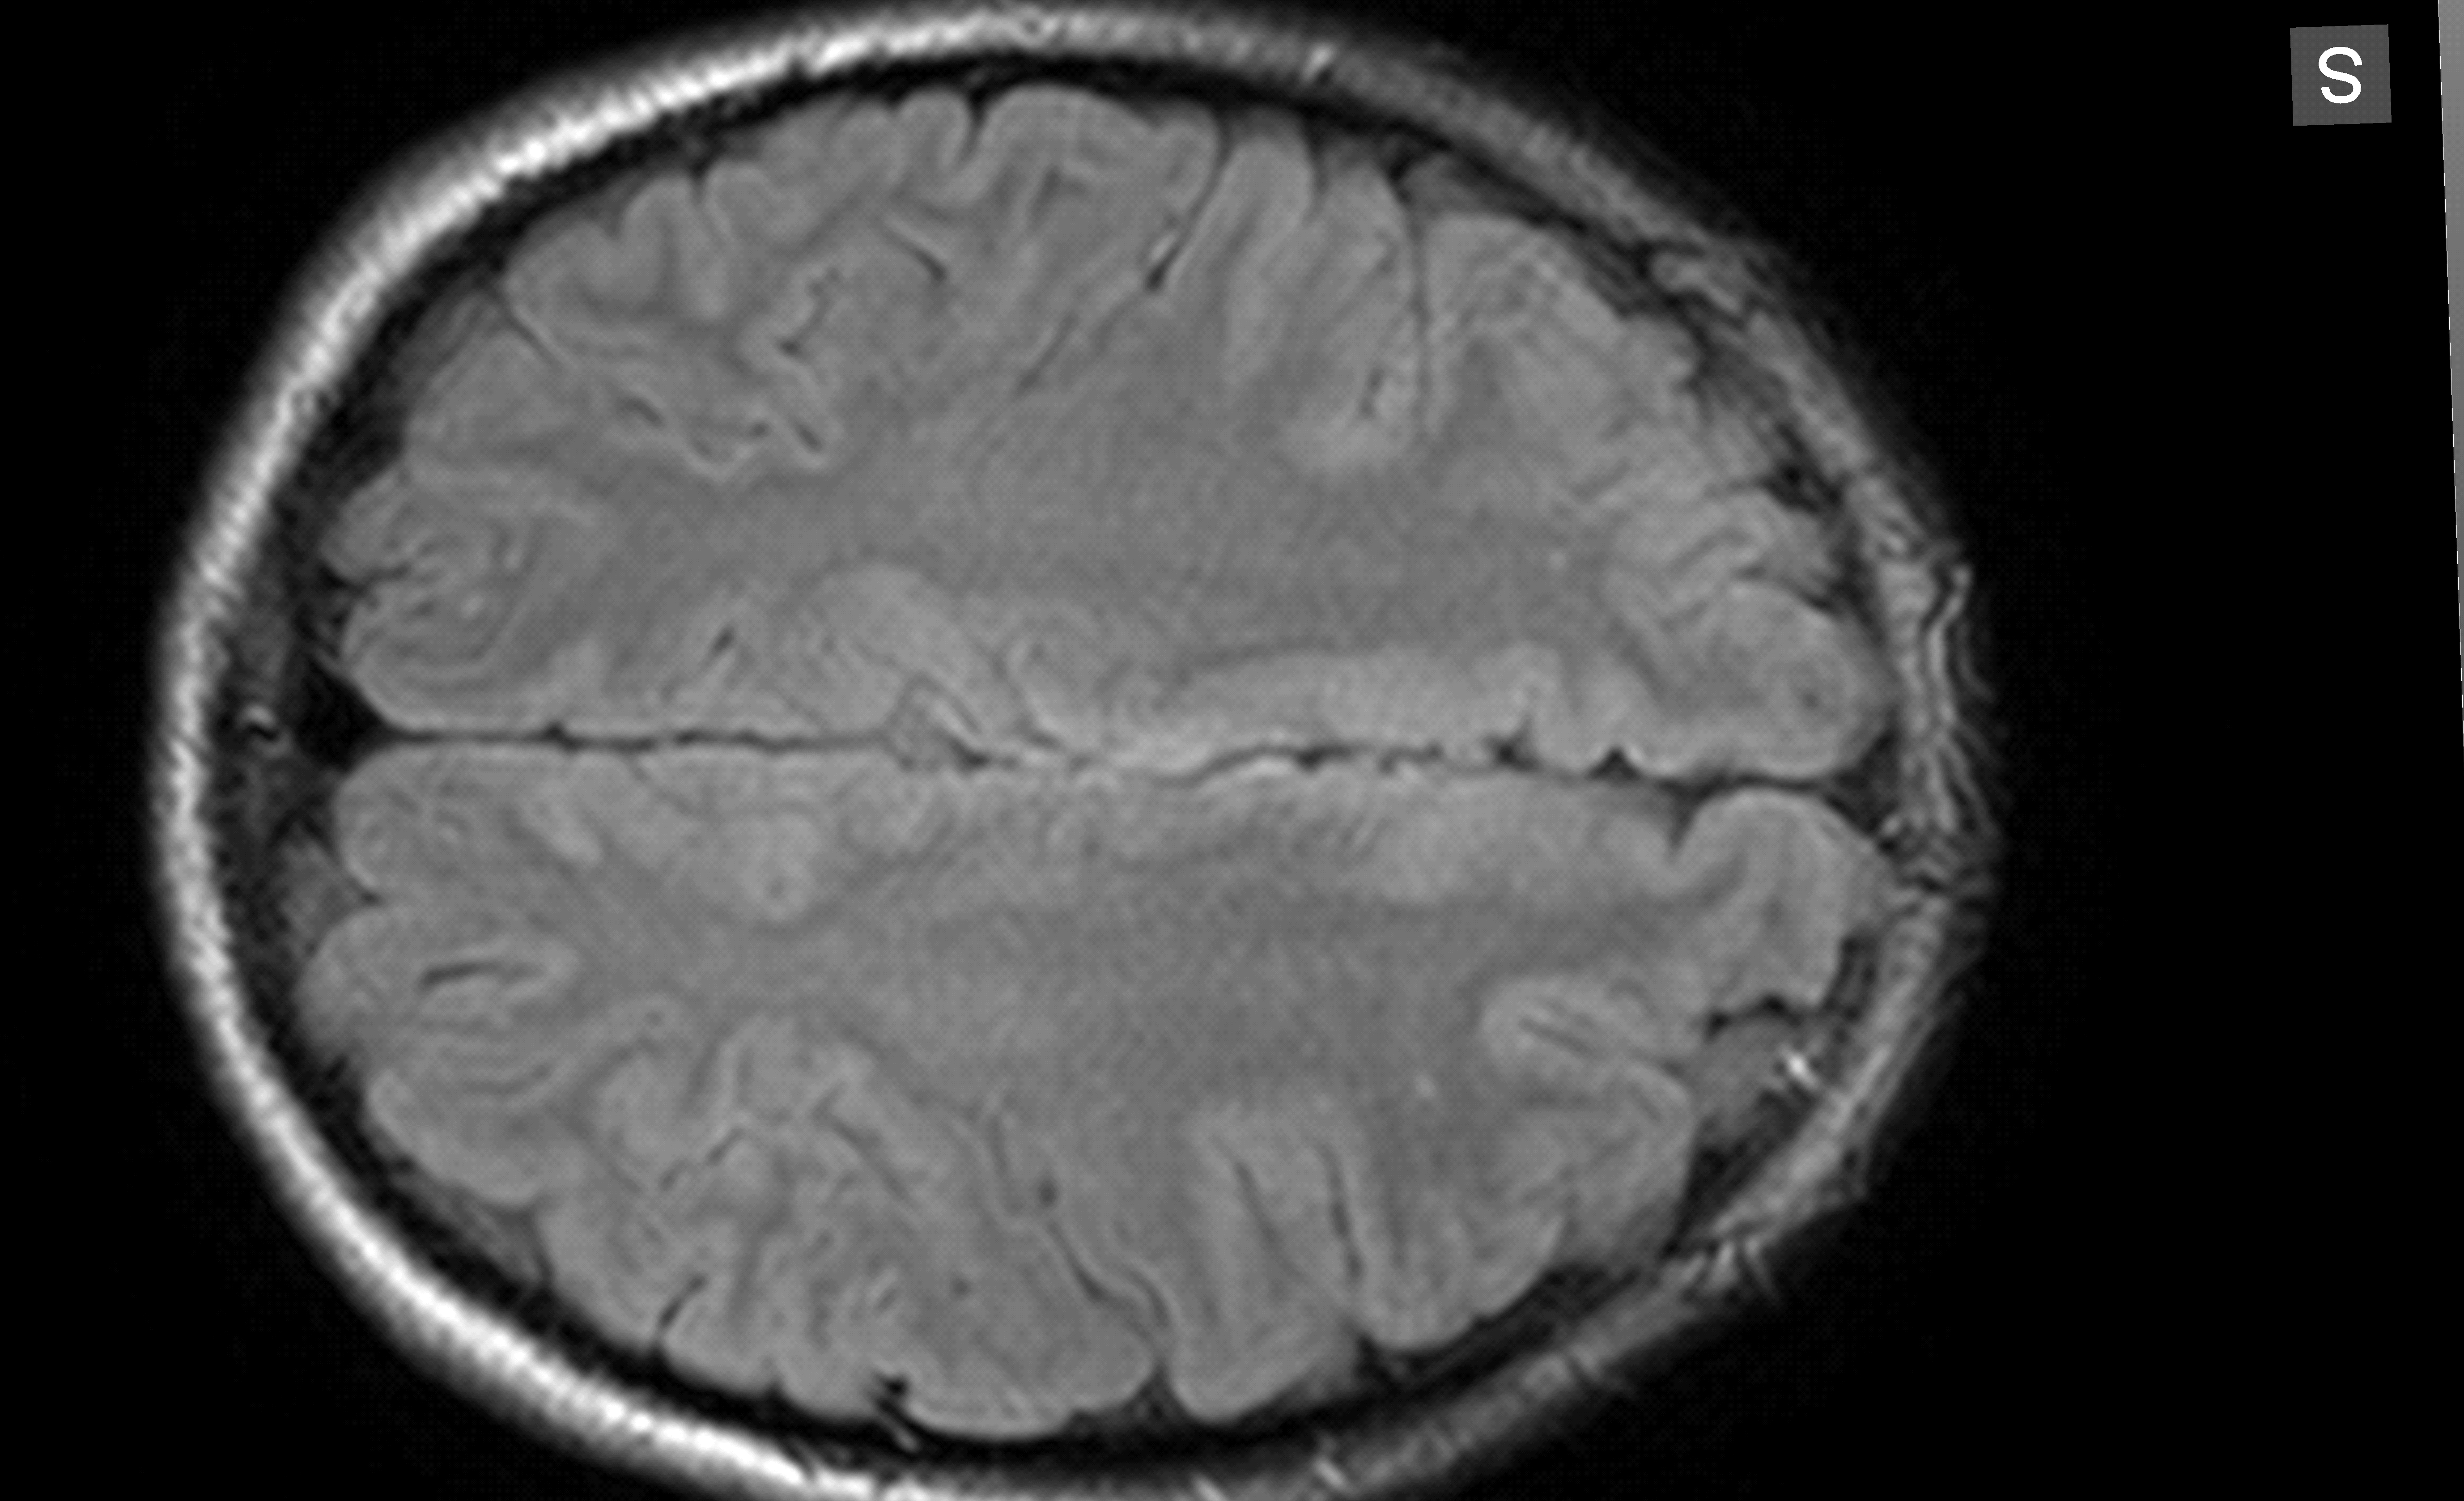
\includegraphics[width=\textwidth]{kmc400/wm_lessions}
		\caption{Flair Image 	\label{fig_white_matter_lessions_a}}
	\end{subfigure}
	\begin{subfigure}{0.45\textwidth}
		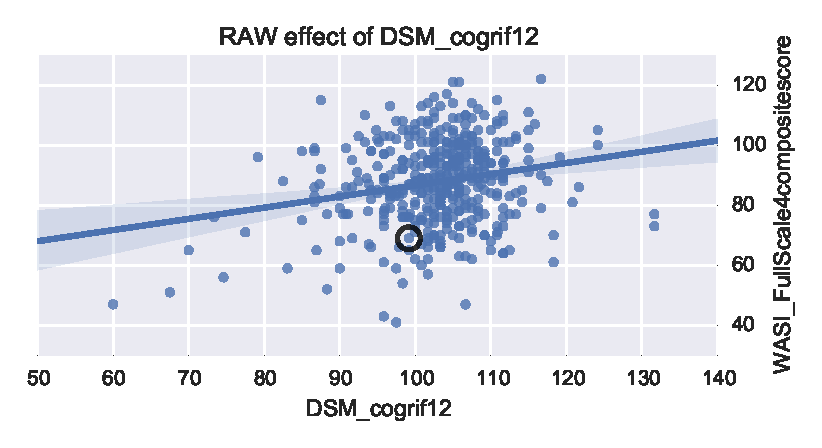
\includegraphics[width=\textwidth]{kmc400/wm_gri_wasi}
		\caption{Plot of Griffiths and WASI scores 	\label{fig_white_matter_lessions_b}}
	\end{subfigure}
	\caption{This subject's white matter lessions probably appeared after birth}
	\label{fig_white_matter_lessions}
\end{figure}


%789
One of the subjects presents a prominent dilation of the supratentorial ventricular system with thinning of the periventricular white matter indicated by FLAIR hypersignal. These findings suggest periventricular leukomalacia caused by lesions in vulnerable areas related to perinatal hypoxia or ischemia in preterms. This subject was indeed born at 31 weeks of gestational age with a weight of 1100 grams. By using a region of interest in the peri-ventricular parietal at the supramarginal gyrus on the right side, the tractography shows a clear alteration in the number and arrangement of fibers (see Figure \ref{fig_homunculus_feet}). There are some transversal, non anatomical fibers, that could indicate brain plasticity. The fibers belonging to the corticobulbar tract appear diminished. In the homuncular representation, these fibers are associated with the feet. At the left side, there are only a few long longitudinal fibers, with a severe diminution of the projection tracts associated with feet and hands. These findings correspond to the clinical diagnosis of the subject, who has spastic cerebral palsy, with right hemiparesis and cerebellar ataxia.  

\begin{figure}
	\centering
	\begin{subfigure}{0.45\textwidth}
		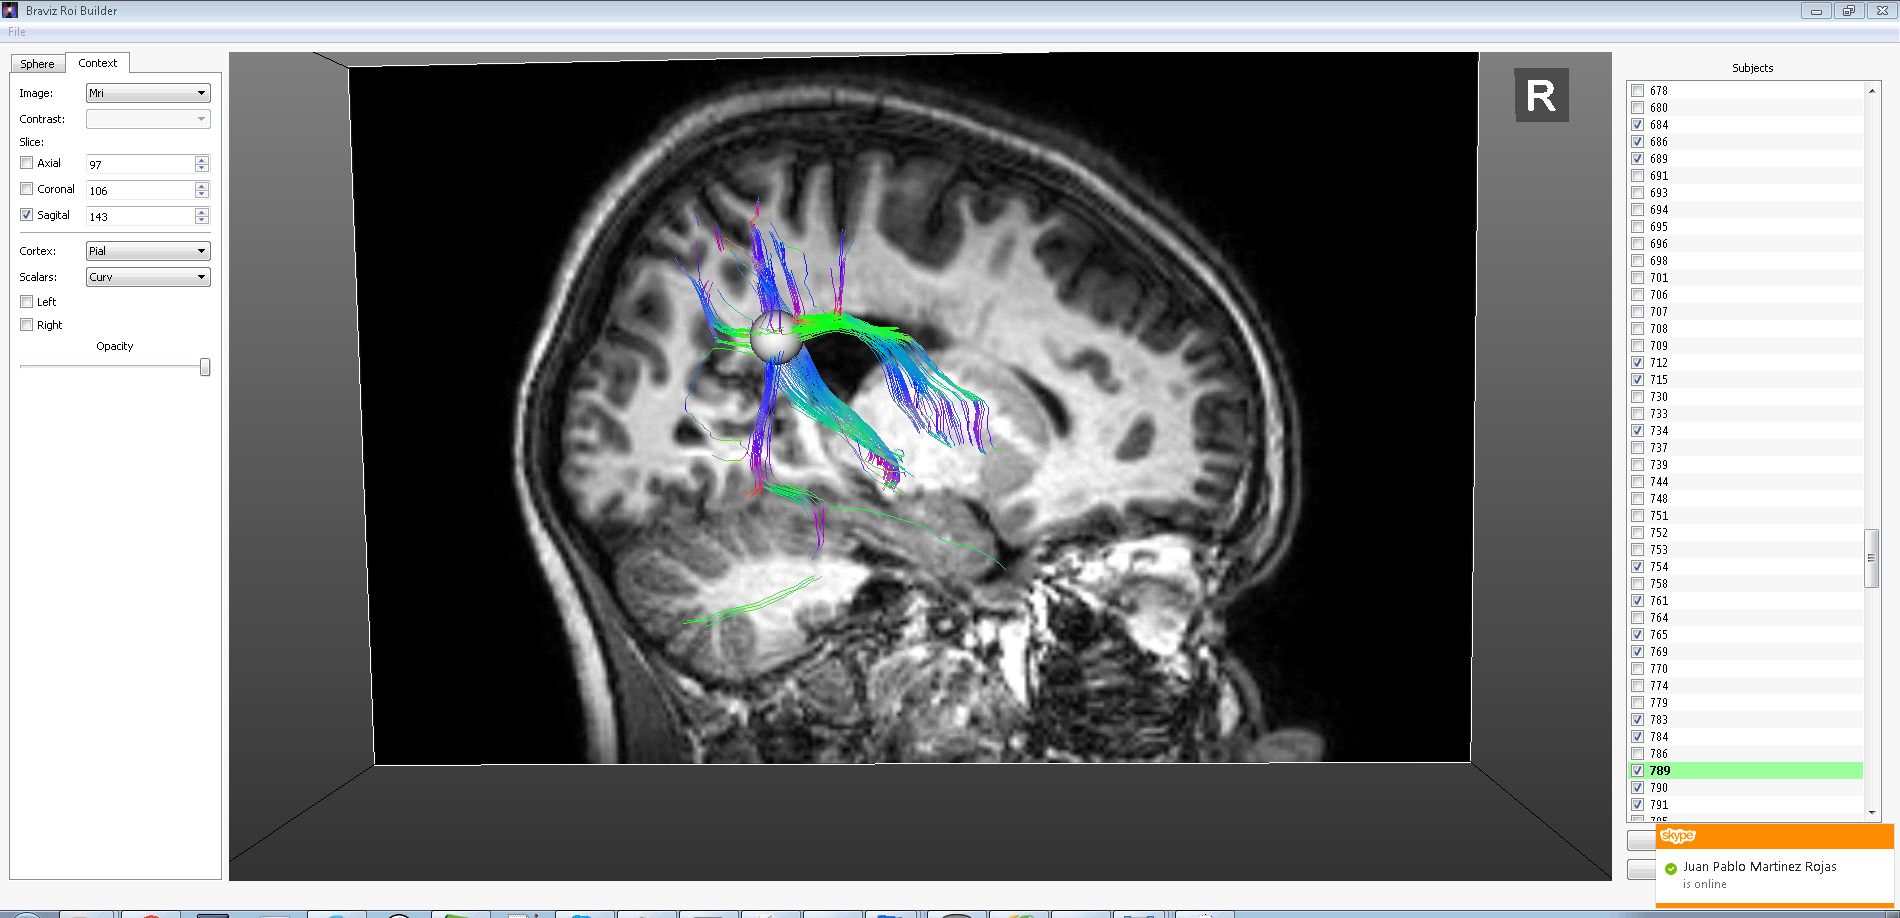
\includegraphics[width=\textwidth, trim=300pt 120pt 350pt 85pt, clip]{kmc400/homunculo_pies_2}
		\caption{Abnormal}
	\end{subfigure}
	\begin{subfigure}{0.45\textwidth}
		\includegraphics[width=\textwidth, trim=300pt 120pt 350pt 85pt, clip]{kmc400/homunculo_pies_control_2}
		\caption{Control}
	\end{subfigure}
	\caption{The motor fibers on subject (a) are reduced, causing alterations in feet movement. A healthy term subject is shown on (b) for comparisson. }
	\label{fig_homunculus_feet}
\end{figure}

%  426
While looking at white matter volumes in the sample, one subject stood out for having a significant lower volume (see Figure \ref{fig_white_matter}). Images showed an increase  in the diploe by hyperostesis of reactive aspect, and an increase in the thickness of temporal muscles (See Figure \ref{fig_diploe}). The cortical atrophy is predominantly parietal and frontal, but the volume of hippocampi and ventricular system is conserved, which indicates a conservation of deep brain fibers. The structural characteristics predict that the subject will have slower thought processes. Clinical data confirms that she has low WASI coefficient of 43, and that she had significant problems completing the nine holes peg test. The clinical diagnosis was a severe psychomotor retardation.


\begin{figure}
	\centering
	\begin{subfigure}{0.45\textwidth}
		\includegraphics[width=\textwidth, trim=700pt 400pt 220pt 150pt, clip]{kmc400/wm_atrophy}
		\caption{Abnormal}
	\end{subfigure}
	\begin{subfigure}{0.45\textwidth}
		\includegraphics[width=\textwidth, trim=700pt 400pt 220pt 150pt, clip]{kmc400/wm_control}
		\caption{Control}
	\end{subfigure}
	\caption{White matter segmentation of a subject with atrophy, next to the white matter of a normal subject for comparison}
	\label{fig_white_matter}
\end{figure}

\begin{figure}
	\centering
	\begin{subfigure}{0.45\textwidth}
		\includegraphics[width=\textwidth, trim=1400pt 0pt 1400pt 0pt, clip]{kmc400/thick_skull}
		\caption{Abnormal}
	\end{subfigure}
	\begin{subfigure}{0.45\textwidth}
		\includegraphics[width=\textwidth, trim=1400pt 0pt 1400pt 0pt, clip]{kmc400/thick_skull_control}
		\caption{Control}
	\end{subfigure}
	\caption{A subject with an abnormal diploe thickness, next to a term subject for comparison}
	\label{fig_diploe}
\end{figure}


\chapter{Braviz usage analysis}
\label{chap_analysis}
%\section{Retrospective}

%¿cómo estabamos al principio?

At the start of this project several image analysis and visualization tools (see chapter \ref{chap_related}) were available. However these tools are designed to work with specific data types, and thus integrating data from different sources required significant work. Additionally most of these tools have a step learning curve, which is appropriate for image experts but leaves them out of reach for users from other domains. Experts from domains different to radiology required to go trough the radiologist or an engineer in order to access image data. Moreover clinical data was always on separate files, which meant it was necessary to switch application in order to get context information about a subject. Typical image based analysis involved extracting scalar features from images, which were later added to a table, and then analyzed in statistical software together with clinical data. This analysis was usually completed using tables. Generating plots required additional steps and was done only for communication purposes. The risk of this approach was that outliers or pathological data could go undetected. 

The current project was conceived to address these issues. Using the proposed tools it is possible to access image data instantaneously,  for image experts, but also for experts from different domains. In addition these images are showed with context and they can be linked to additional information of a given subject. Scalar features extracted from image data can be visually analyzed together with clinical data. In this way outliers immediately draw attention, can be identified and analyzed in more detail. Experts from all domains can access spatial data, think about it, and propose analyzes. In contrast, before most analyzes involving spatial data were proposed by image experts and limited to existing tools. These analyzes will still need the help of image experts for performing the required calculations and interpreting the results; and possibly from engineers if new tools need to be developed. By making data available to the whole team, this way of thinking becomes possible.    

% ¿Como ha anvanzado nuestra comprension del problema?
% ¿de los datos?
% ¿de los usuarios?
% ¿de las necesidades?
In order to better assess the benefits and limitations of the proposed approach, we conducted several interviews with potential users, applied surveys, and did a group session. These activities and their results will be explained in this chapter. Additionally it will show how the model from Chapter \ref{chap_model} is reflected in the system's applications.	

% ¿qué problemas nuevos han surgido?
% ¿qué oportunidades?
% ¿hacia dónde vamos?

\section{Collaboration with Team Cave}

\footnote{A better name is needed, help Cyril} An important part of the requirements analysis for the project was carried out at CHUL in Quebec, Canada. Specifically, the Axes Neurosciences group was a significant contributor. This group researches the functioning of the nervous system in healthy and pathological conditions. One of the methods used is performing experiments on large numbers of participants. During these experiments they collect data from each participant using neuro-psychological tests, measurements of muscle strength and movement, neuro-image and TMS tests. This center is located inside the Laval Universiy Hospital (CHUL) in Quebec.

Single or double TMS was being used for measuring the quality of nerve fibers, and repetitive TMS was being used as therapy on muscles \footnote{Maybe cite Veronique's paper as an example}. Data from TMS experiments was captured using EEG equipment and the \emph{Lab Chart} software. These signals were then post processed in the same software and scalar measures were extracted. These measurements were then copied to an excel table where they were combined with subject data and other collected variables; for example the feeling of pain, the strength of a muscle, or the time taken for completing a nine hole peg test. Afterward the excel table would be re-organized and fed into statistical software. The main statistical software used at this stage were \emph{Statistica} and \emph{Prism}. Recently the lab acquired a license for \emph{Aabel}, which some researchers like better as it provides very good explanations of the meaning and methods of each analysis. Also the manual is rich with statistical theory and examples. The tool also provides interactive graphs which can be used for exploratory analysis. Notice that some of the software is proprietary and there were limited licenses, therefore it was common for researchers to have to move data trough different machines using usb drives. Internet was not an option as the hospital network is very restrictive.

%Description of the lab, software used, prism, aabel, statistica, labchart, excel, 

Can I add some pictures from Cyril lab ?

% Knwoldedge depends on the hypotheses, and the hypotheses on the technology available for testing the questions raised. 
 
% Cyril's team
% Cyril's TMS publication

%The tms applications

One of the interests of the group was analyzing relationships between TMS outcomes and white matter structure as portrayed by DWI and tractography. The particular TMS experiment tested the connections from the primary motor cortex to the hand muscles, and between the motor cortices at both hemipsheres (see \autocite{schneider_cerebral_2012}). For this purpose an specific application was designed, it showed the values of the TMS outcome together with visualizations of the relevant fiber bundles. Screen-shots of the finished application can be seen on figures \ref{fig_tms_1} and \ref{fig_tms_2}). 

\begin{figure}
	\centering
		\includegraphics[width=0.90\textwidth]{figures/analysis/tms_view_early}
	\caption{An early version of the TMS viewer application.}
	\label{fig_tms_view_early}
\end{figure}

Figure \ref{fig_tms_view_early} shows an earlier version of the application. In the top left side it had a combo-box for selecting one of the different outcomes. The radio buttons below allowed the researcher to choose between the metrics for the dominant or non-dominant side. Finally there was a list of subjects which could be filtered to show only males, only females or both. At the top right there was a 3D viewer which would display a relevant fiber bundle related to the current outcome. Specifically for intra-cortical measures it would show the motor fibers for the corresponding hemisphere (as in figure \ref{fig_tms_1}) while the corpus callosum would appear for Inter-hemispheric measures.
Below there was a bar plot showing the values of the current outcome for the current subject, together with a large display of this value on the right. The solid and dotted lines in the plot correspond to the mean and the interval within one standard deviation; these statistics are calculated considering only the subjects in the control group. Bars inside this interval are colored green while those outside are colored in red.
This layout was first designed on paper with one of the group researchers. 

The user could move trough subjects either by selecting a code on the list or by clicking on one of the bars. The bar at the right would change to the new value, using a transition to accentuate the difference. The image will also change to that of the new subject. This simple tool allows the researcher to navigate between the TMS-outcomes while looking at the underlying white matter structure. 

\begin{figure}
	\centering
		\includegraphics[width=0.90\textwidth]{figures/analysis/tms_view_motor}
	\caption{A second version of the TMS-viewer application}
	\label{fig_tms_view_second}
\end{figure}

Figure \ref{fig_tms_view_second} shows a posterior version of this tool. After receiving feedback from the group, several improvements were made:
\begin{itemize}
	\item TMS outcomes are now organized in a tree, and more descriptive names are used. The purpose is to provide meaning to experts who have limited experience with TMS. Additionally tooltips were added in order to provide additional information on each metric.
	\item The underlying study involved three groups: kangaroo mother care, incubator and control. For some analysis it is convenient to be blind about these groups, but some other times it is beneficial to have this information. Now there is an option to show the different groups in the list of subjects by using different background colors.
	\item The axes in the plot are more clearly labeled and measurement units are shown. 
	\item For some outcomes a higher value is better, while for some others a lower value is better. Now values of the second type are showed using squares instead of bars.
	\item Colors in the main plot were redefined. Now red can be read as \emph{worst than controls}, yellow as \emph{similar to controls} and green as \emph{better than controls}.
	\item The main plot can show the complete sample or only some interesting subjects. The user may add or remove subjects to this sub-sample using the buttons below the subject list.
\end{itemize}

Another round of feedback produced the version shown in figure \ref{fig_tms_2}. This version included additional information in the 3D viewer in order to help users interpret it. The other major feature was showing grouped data in the main plot for the three groups in the study.

This tool allowed experts to .................\footnote{Help Cyril}.


% Veronique Manip
% finding correlations

Another common task found in several of the current experiments was finding correlations between dependent variables. This process was usually done by testing each pair of variables at a time, but \emph{Aabel} provided a correlation matrix. This idea was nice, but it could be improved. In a group with several young researchers\footnote{Vero, Hugo, LD} an application for testing correlations was designed. The result of this effort is the \emph{Correlations} application shown in figure \ref{fig_correlations}. This application is now included in the Braviz set, but can also be used as a stand-alone application (available at \url{https://github.com/diego0020/correlation_viewer}). In the stand-alone mode the application loads data from an excel file where each row is a subject and each column a variable. The tool interface is divided in three. The first component is a list of variables, each of them with a check-box; it is used to add or remove variables from the analysis. Next is a correlation matrix which encodes in colors the degree of correlation between each pair of variables. And finally, when the user clicks on a square of the matrix the corresponding scatter plot is shown together with the $r$ and $p$ values from the Pearson correlation. An important feature is that individual points can be removed from analysis by clicking on them in the scatter plot. This feature was added because commonly there are extreme cases which give the impression of a high correlation, however this effect disappears when the point is removed. The application was refined trough several feedback sessions in the group, and several bugs were discovered and corrected.  This tool is now currently used in this lab\footnote{maybe ask hugo, v and ld from some experineces}. Below is a testimony from one of the researchers \footnote{hugo}.

\begin{quote}
During the last year, I had the chance to test the new computer program named CorrelationViewer. This program allows visualizing correlations between multiple series of variables. For instance, in my last study, I tested several outcomes that improved after a treatment. I used CorrelationViewer to determine whether my outcomes changes could be related to each other. An interesting feature is the colour scale allowing a quick recognition of the outcomes related altogether. Indeed, this colour scale (gradient red to gradient blue) informs firstly about the direction of the correlation (positive vs. negative). Also, the possibility to visualize easily each linear regression by clicking directly on the wanted correlation is important and practical. You can look at the correlation distribution and whether few participants drive the relation. Above the graph, the p and r stats allow me to determine rapidly whether this graph is pertinent in my research project. Finally, another interesting feature is the possibility to click on a point in the graph and to exclude it from the relation. In this case, new p and r stats are automatically calculated. It allows spotting and excluding easily potential outliers from the project.

With CorrelationViewer, I spent less time to handle the data from one program to the other and I could detect easily and quickly the outcomes correlated altogether. It is an easy and practical tool to use when I do my stats. 
\end{quote}

The \emph{Anova} and \emph{Linear Model} applications (see figures \ref{fig_anova_2} and \ref{fig_lm_2}) were also inspired but the current research questions and workflows in this team. Most of the time they have a treatment variable, several confounders, and outcomes; and the objective is assessing if the treatment has any effects after controlling for confounders. This is usually done using ANOVA or two way ANOVA if before and after data is available. The two way ANOVA feature has not been implemented in the main Braviz tool, but is in the list of wanted features \footnote{what else can be said here?}. 

% Anna Belle Manip
% Hugo Manip
% 
% ANOVA - LM

% Alyssa

A pediatrician\footnote{Alyssa} who worked at the hospital provided her opinion of the system from the clinical point of view. She thought that such a tool would be very useful in order to talk the kid's parents, and better explain any findings. Also if the sample from the current study showed positive results in a similar case, this evidence could be shared with parents to reassure them. It would be also helpful to have all data from a given subject as well as reference data in order to understand the factors that affect a prognosis. 

%insights from cyril's interview
% Visuals are very important. 

In a follow up interview with the head of the lab (Cyril\footnote{Should Cyril be named explicitly?}) he gave us his impressions about the complete system. First of all he was concerned about how new users could get up to speed. He proposed that the first screen should guide the user. What should he do first? There should be a tutorial, and it should be enough so that the user can beyond intuitively. Additionally, he expressed that the user should never be puzzled by the tool itself. This means that the main format should be consistent. There should not be any surprises. The tool should also provide some guidance on relevant data for specific questions. 

As a possible application, he stated that the tool should help in understanding subjects which are not part of the original sample. Given a new subject, it should help me find similar subjects in the sample. It would be specially useful if there are no images of the new subject but the images of existing subjects with similar characteristics are available. 

He also emphasized that this system should be targeted to multiple users expert in multiple domains. The point was not transforming each user into an expert in everything, but to help experts work together and provide a full picture of each subject. With current technologies data from different domains are out of reach, because tools are not compatible, it's hard to understand, and the links between domains are not evident. This causes subjects to be divided into different dimensions. To counter this it is necessary to use a common language that makes links easier to see. By looking at each subject as a whole the tool humanizes research. In this way Braviz could also be very valuable in teaching. 

The tool should let users be very efficient at their work and never make them waste time. It should also be very accurate, as any mistake would cause experts to loose trust in the tool, and all benefits would be lost. No one would want to use a tool that produces results that must be double checked.

He agreed with the user centered approach, and remarked that tools should for end-users should be designed by those end-users, but engineers would always be required.

A final remark was that \emph{knowledge depends on the hypotheses, and the hypotheses on the technology available for testing the questions raised}. 


%%
%KMC
%	Marin
%	Rejean
%	Nathalie

% Video Conference from Iowa
% D:\dropbox\Dropbox\VaBD\ProyectoSavingBrains\minutas_demos_04_14.odt
% Ste Irenne

% lock patient

\section{Interest Surveys}
NIDCAP
Guttman's lab

In order to evaluate the interest of the community for a tool such as Braviz, a survey was administered at the NIDCAP\footnote{Por favor verificar con Nathalie} conference.  This conference was held in Barcelona on October 26, 2014. 
Assistants to the conference were ......................................\footnote{Help}. Seven experts answered.

Before the survey, Dr Charpak gave a demonstration of the tool. The first part of a question asked participants how much they agreed with a set of statements, using a likert scale. The results from this question can be seen in table \ref{tab_nidcap_likert}. 

\begin{table}
	\centering
		\begin{tabular}{p{0.6\textwidth}ccccc}
			\toprule
			Statement&1&2&3&4&5 \\
			\midrule
			The presented tools (Braviz) would support my line of work. & 5 &-&-& 2 &- \\
			Interactive visualization with access to individual detailed information is a key feature. &7&-&-&-&- \\			
			The possibility to explore images (MRI, DTI, fMRI) in the context of other variables, adds value to the analysis. &7&-&-&-&- \\
			The integration of basic statistical tools to the interactive exploration is a valuable feature &7&-&-&-&- \\
			I would be willing to test these tools using my own data in a near future (months) & 6 &-& 1 &-&- \\
			\bottomrule
		\end{tabular}
	\caption{Answers to the survey applied at NIDCAP, 2014. In the first part of the survey, participants should indicate how much they agreed with the listed statements. The scale was
	1: Totally agree, 2: Agree, 3: Neutral, 4: Disagree and 5: Totally disagree. The table shows the number of participants who answered with each value.}
	\label{tab_nidcap_likert}
\end{table}

The second question was: With what frequency do you make visualizations of your data? The possible answers and the number of participants who selected them were:

\begin{itemize}
	\item It's always the first thing I do : No one
	\item Almost always: four participants
	\item Only when I notice something odd: one participants
	\item Rarely: one participant
	\item Just to publish or socialize results: No one
\end{itemize}

The following questions asked : Which tools, similar to the one presented, do you know of? and how satisfied are you with these tools? The answers were 
\begin{itemize}
	\item Conventional T1, T2, MRI, DWI, FA. Very satisfied.
	\item Computarized order entry ( CPOE ). Very satisfied.
	\item Not a single tool, but several specialized tools: cognitive potentials, tractography, etc. Very satisfied.
\end{itemize}

The rest of participants left this space empty. The next question asked: What additional features would you like to find in a visual exploration tool? Participants wrote the following answers
\begin{itemize}
	\item Templates. Volume of structures and tractography data are best if used to combine with functional data in the follow up activity. 
	\item Vermis volumetric analysis.
	\item New techniques as analysis of electical activity using EEG and Bayley III curves for followup. 
	\item Orthogonal visualization of brains, ordinal variables, anova with nominal and ordinal outcomes, comparison with standard values.
\end{itemize}

This survey was also applied at the Center for Neurological Images at Brigham and Women's hospital in Botson, MA, USA. This activity was conducted on June, 2015. The methodology was also a quick demo followed by the survey. This group is composed of physicians (neurologists and radiologists), biologists and engineers, who work in brain image research. 

\begin{table}
	\centering
		\begin{tabular}{p{0.6\textwidth}ccccc}
			\toprule
			Statement&1&2&3&4&5 \\
			\midrule
			The presented tools (Braviz) would support my line of work. & 1 & 3 &-& - & - \\
			Interactive visualization with access to individual detailed information is a key feature. &4&-&-&-&- \\			
			The possibility to explore images (MRI, DTI, fMRI) in the context of other variables, adds value to the analysis. &4&-&-&-&- \\
			The integration of basic statistical tools to the interactive exploration is a valuable feature &4&-&-&-&- \\
			I would be willing to test these tools using my own data in a near future (months) & 3 & 1 & - &-&- \\
			\bottomrule
		\end{tabular}
	\caption{Answers to the survey applied at BWH, 20145. See table \ref{tab_nidcap_likert}.}
	\label{tab_bwh_likert}
\end{table}

The answers to the following questions were

\begin{itemize}
	\item With what frequency do you make visualizations of your data?
	\begin{itemize}
		\item It's always the first thing I do : one participant
		\item Almost always: two participants
		\item Rarely one participant
	\end{itemize}
	\item Which tools similar to the one presented, do you know of? How satisfied are you with these tools?
	\begin{itemize}
		\item Sear, very satisfied
		\item Spine, very satisfied
	\end{itemize}
	\item What additional features would you  like in a visual exploration tool?
	\begin{itemize}
		\item Interactive feature selection (for example all white matter lesions)
		\item Atlases, multiple statistics module (for both descriptive and analysis), database selection \& matching tools, export results and images, voxel-wise analysis, TBSS.
	\end{itemize}	
\end{itemize}

\smallskip

While the sample is small, the survey shows there are multiple specialists willing to try these tools. Most of the participants consider visualization an essential part of analysis, and find value in integrating spatial and clinical data. On the other hand none of them complained about the tools they currently use. This supports our hypothesis that Braviz will not replace any of these tools but complement them. Additionally the survey shows that there is a large interest in integrating more data types and statistical analyzes. Finally, several of the experts are willing to participate in longer studies, so in the future we will be able to collect more data about how these tools can be used in diverse projects.


\section{Group Test}

Ana Maria

\section{Feature Model}

%Consequence of the model

The process used to build applications for the Braviz suite is based on the feature model described in chapter \ref{chap_model}. This model presents the commonalities and variability inside the set of applications. The Braviz library provides a set of reusable components that can be used to streamline the construction of new applications. The model of figure \ref{fig_feature_problem} describes the design space at the problem level. It is independent of an application and is best used to design new applications at a high level. This model should be used in the early stages of application design. 

The model represented in figure \ref{fig_feature_solution} is a low level model, coupled with the current implementation. It should be used after the problem space model in order to define the best option to implement the required set of features. 

\begin{table}
\scriptsize
\begin{tabular}{llllllllllllllll}
\toprule
{} & \rot{RoiBuilder} & \rot{LogicBundles} & \rot{LinearMeasure} & \rot{subjOverview} & \rot{sampleOverview} & \rot{CheckRegistration} & \rot{ExploreFMRI} & \rot{Anova} & \rot{LinearModel} & \rot{Histogram} & \rot{Correlations} & \rot{ParallelCoordinates} & \rot{SubjectSwitcher} & \rot{CalculateFeatures} & \rot{PopulateCache} \\
\midrule
SpatialVis           &       \checkmark &         \checkmark &          \checkmark &         \checkmark &           \checkmark &              \checkmark &        \checkmark &             &                   &                 &                    &                           &                       &                         &                     \\
Two                  &                  &                    &                     &                    &                      &                         &                   &             &                   &                 &                    &                           &                       &                         &                     \\
Three                &       \checkmark &         \checkmark &          \checkmark &         \checkmark &           \checkmark &              \checkmark &        \checkmark &             &                   &                 &                    &                           &                       &                         &                     \\
Images               &       \checkmark &         \checkmark &          \checkmark &         \checkmark &           \checkmark &              \checkmark &        \checkmark &             &                   &                 &                    &                           &                       &                         &                     \\
Surfaces             &       \checkmark &         \checkmark &                     &         \checkmark &           \checkmark &                         &        \checkmark &             &                   &                 &                    &                           &                       &                         &                     \\
Tractography         &       \checkmark &         \checkmark &                     &         \checkmark &           \checkmark &                         &                   &             &                   &                 &                    &                           &                       &                         &                     \\
Segmentation         &                  &                    &                     &         \checkmark &           \checkmark &                         &                   &             &                   &                 &                    &                           &                       &                         &                     \\
NonSpatialVis        &                  &                    &                     &                    &           \checkmark &                         &        \checkmark &  \checkmark &        \checkmark &      \checkmark &         \checkmark &                \checkmark &                       &                         &                     \\
Bars                 &                  &                    &                     &                    &           \checkmark &                         &                   &             &                   &                 &                    &                           &                       &                         &                     \\
Scatter              &                  &                    &                     &                    &                      &                         &                   &  \checkmark &        \checkmark &                 &         \checkmark &                           &                       &                         &                     \\
Histogram            &                  &                    &                     &                    &                      &                         &                   &             &                   &      \checkmark &                    &                           &                       &                         &                     \\
BoxPlot              &                  &                    &                     &                    &                      &                         &                   &  \checkmark &                   &                 &                    &                           &                       &                         &                     \\
Spider               &                  &                    &                     &                    &                      &                         &                   &             &                   &                 &                    &                           &                       &                         &                     \\
TimeLine             &                  &                    &                     &                    &                      &                         &        \checkmark &             &                   &                 &                    &                           &                       &                         &                     \\
ParallelCoordinates  &                  &                    &                     &                    &                      &                         &                   &             &                   &                 &                    &                \checkmark &                       &                         &                     \\
SaveRestore          &       \checkmark &         \checkmark &          \checkmark &         \checkmark &           \checkmark &                         &        \checkmark &  \checkmark &        \checkmark &                 &                    &                           &                       &                         &                     \\
Log                  &       \checkmark &         \checkmark &          \checkmark &         \checkmark &           \checkmark &                         &        \checkmark &  \checkmark &        \checkmark &                 &                    &                \checkmark &                       &                         &                     \\
SendSample           &                  &                    &                     &         \checkmark &           \checkmark &                         &        \checkmark &  \checkmark &        \checkmark &                 &         \checkmark &                \checkmark &            \checkmark &                         &                     \\
SendSubject          &                  &                    &                     &         \checkmark &           \checkmark &                         &        \checkmark &  \checkmark &        \checkmark &                 &         \checkmark &                \checkmark &            \checkmark &                         &                     \\
SendVisualization    &                  &                    &                     &         \checkmark &                      &                         &                   &             &                   &                 &                    &                           &                       &                         &                     \\
SendVariables        &                  &                    &                     &                    &                      &                         &                   &  \checkmark &        \checkmark &                 &                    &                           &                       &                         &                     \\
ReceiveSample        &                  &                    &                     &         \checkmark &           \checkmark &                         &        \checkmark &  \checkmark &        \checkmark &      \checkmark &         \checkmark &                \checkmark &            \checkmark &                         &                     \\
ReceiveSubject       &                  &                    &                     &         \checkmark &           \checkmark &                         &        \checkmark &  \checkmark &        \checkmark &      \checkmark &         \checkmark &                \checkmark &            \checkmark &                         &                     \\
ReceiveVisualization &                  &                    &                     &                    &           \checkmark &                         &                   &             &                   &                 &                    &                           &                       &                         &                     \\
ReceiveVariables     &                  &                    &                     &                    &                      &                         &                   &             &                   &                 &         \checkmark &                \checkmark &                       &                         &                     \\
Graphical            &       \checkmark &         \checkmark &          \checkmark &         \checkmark &           \checkmark &              \checkmark &        \checkmark &  \checkmark &        \checkmark &      \checkmark &         \checkmark &                \checkmark &            \checkmark &                         &                     \\
CommandLine          &                  &                    &                     &                    &                      &                         &                   &             &                   &                 &                    &                           &                       &              \checkmark &          \checkmark \\
DefineRegions        &       \checkmark &                    &                     &                    &                      &                         &                   &             &                   &                 &                    &                           &                       &                         &                     \\
ManualMeasure        &                  &                    &          \checkmark &                    &                      &                         &                   &             &                   &                 &                    &                           &                       &                         &                     \\
ManualSegmentation   &                  &                    &                     &                    &                      &                         &                   &             &                   &                 &                    &                           &                       &                         &                     \\
Filter               &       \checkmark &         \checkmark &                     &         \checkmark &           \checkmark &                         &        \checkmark &             &                   &                 &                    &                           &                       &              \checkmark &          \checkmark \\
Isosurfaces          &                  &                    &                     &         \checkmark &           \checkmark &                         &        \checkmark &             &                   &                 &                    &                           &                       &              \checkmark &          \checkmark \\
Transform            &                  &         \checkmark &          \checkmark &         \checkmark &           \checkmark &              \checkmark &        \checkmark &             &                   &                 &                    &                           &                       &              \checkmark &          \checkmark \\
LinearModels         &                  &                    &                     &                    &                      &                         &                   &  \checkmark &        \checkmark &                 &         \checkmark &                           &                       &                         &                     \\
Classification       &                  &                    &                     &                    &                      &                         &                   &             &                   &                 &                    &                           &                       &                         &                     \\
Clustering           &                  &                    &                     &                    &                      &                         &                   &             &                   &                 &                    &                           &                       &                         &                     \\
NonParametric        &                  &                    &                     &                    &                      &                         &                   &             &                   &                 &                    &                           &                       &                         &                     \\
\bottomrule
\end{tabular}
	
\caption{\label{tab_features_problem} Configurations of the current applications in relation to the problem space feature model( see figure \ref{fig_feature_problem}).}
\end{table}

Table \ref{tab_features_problem} shows the features from the problem space model used in the applications available in the current version. Applications are sorted from left to right based on their categories. First are the applications that allow users to generate new data based on images, followed by the applications designed to explore spatial data, then those designed to explore tabular data and perform statistical analyzes and finally some command line utilities that can be used to prepare data for analysis. Some of the features are not yet used in any applications, but they will probably be needed in future developments. Specifically there is evidence of the need to integrate more advanced statistical and machine learning functions to aid in the analysis. 

\begin{table}
\scriptsize
\begin{tabular}{llllllllllllllll}
\toprule
{} & \rot{RoiBuilder} & \rot{LogicBundles} & \rot{LinearMeasure} & \rot{subjOverview} & \rot{sampleOverview} & \rot{ExploreFMRI} & \rot{CheckRegistration} & \rot{Anova} & \rot{LinearModel} & \rot{Correlations} & \rot{Histogram} & \rot{ParallelCoordinates} & \rot{SubjectSwitcher} & \rot{CalculateFeatures} & \rot{PopulateCache} \\
\midrule
CommandLine          &                  &                    &                     &                    &                      &                   &                         &             &                   &                    &                 &                           &                       &              \checkmark &          \checkmark \\
Web                  &                  &                    &                     &                    &                      &                   &                         &             &                   &                    &      \checkmark &                \checkmark &            \checkmark &                         &                     \\
D3                   &                  &                    &                     &                    &                      &                   &                         &             &                   &                    &      \checkmark &                \checkmark &                       &                         &                     \\
Bootstrap            &                  &                    &                     &                    &                      &                   &                         &             &                   &                    &                 &                \checkmark &            \checkmark &                         &                     \\
three                &                  &                    &                     &                    &                      &                   &                         &             &                   &                    &                 &                           &                       &                         &                     \\
DesktopGUI           &       \checkmark &         \checkmark &          \checkmark &         \checkmark &           \checkmark &        \checkmark &              \checkmark &  \checkmark &        \checkmark &         \checkmark &                 &                           &                       &                         &                     \\
MatplotLib           &                  &                    &                     &                    &           \checkmark &        \checkmark &                         &  \checkmark &        \checkmark &         \checkmark &                 &                           &                       &                         &                     \\
VTK                  &       \checkmark &         \checkmark &          \checkmark &         \checkmark &           \checkmark &        \checkmark &              \checkmark &             &                   &                    &                 &                           &                       &                         &                     \\
QtModels             &       \checkmark &         \checkmark &                     &         \checkmark &                      &        \checkmark &                         &  \checkmark &        \checkmark &         \checkmark &                 &                           &                       &                         &                     \\
ReusableQtComponents &       \checkmark &         \checkmark &          \checkmark &         \checkmark &           \checkmark &        \checkmark &              \checkmark &  \checkmark &        \checkmark &         \checkmark &                 &                           &                       &                         &                     \\
SampleManager        &       \checkmark &         \checkmark &          \checkmark &         \checkmark &           \checkmark &        \checkmark &                         &  \checkmark &        \checkmark &         \checkmark &                 &                           &                       &                         &                     \\
ImageManager         &       \checkmark &         \checkmark &          \checkmark &         \checkmark &           \checkmark &        \checkmark &              \checkmark &             &                   &                    &                 &                           &                       &                         &                     \\
ContextPanel         &                  &                    &                     &         \checkmark &                      &                   &                         &             &                   &                    &                 &                           &                       &                         &                     \\
VariableSelectDialog &                  &                    &                     &         \checkmark &           \checkmark &        \checkmark &                         &  \checkmark &        \checkmark &                    &                 &                           &                       &                         &                     \\
Variables            &       \checkmark &                    &          \checkmark &         \checkmark &           \checkmark &        \checkmark &                         &  \checkmark &        \checkmark &         \checkmark &      \checkmark &                \checkmark &                       &                         &                     \\
Samples              &       \checkmark &         \checkmark &          \checkmark &         \checkmark &           \checkmark &        \checkmark &                         &  \checkmark &        \checkmark &         \checkmark &      \checkmark &                \checkmark &            \checkmark &                         &                     \\
Annotations          &                  &                    &                     &         \checkmark &                      &                   &                         &             &                   &                    &                 &                           &                       &                         &                     \\
Images               &       \checkmark &         \checkmark &          \checkmark &         \checkmark &           \checkmark &        \checkmark &              \checkmark &             &                   &                    &                 &                           &                       &              \checkmark &          \checkmark \\
PolyData             &       \checkmark &         \checkmark &          \checkmark &         \checkmark &           \checkmark &        \checkmark &                         &             &                   &                    &                 &                           &                       &              \checkmark &          \checkmark \\
Segmentations        &                  &         \checkmark &          \checkmark &         \checkmark &           \checkmark &                   &                         &             &                   &                    &                 &                           &                       &              \checkmark &          \checkmark \\
Tractography         &       \checkmark &         \checkmark &          \checkmark &         \checkmark &           \checkmark &                   &                         &             &                   &                    &                 &                           &                       &              \checkmark &          \checkmark \\
Surfaces             &       \checkmark &         \checkmark &          \checkmark &         \checkmark &           \checkmark &                   &                         &             &                   &                    &                 &                           &                       &              \checkmark &          \checkmark \\
Contours             &                  &                    &          \checkmark &         \checkmark &           \checkmark &        \checkmark &                         &             &                   &                    &                 &                           &                       &              \checkmark &          \checkmark \\
VTKFilters           &       \checkmark &         \checkmark &                     &         \checkmark &                      &        \checkmark &                         &             &                   &                    &                 &                           &                       &              \checkmark &                     \\
ScipyNumpy           &                  &                    &                     &                    &                      &                   &                         &             &                   &                    &                 &                           &                       &                         &                     \\
R                    &                  &                    &                     &                    &                      &                   &                         &  \checkmark &        \checkmark &         \checkmark &                 &                           &                       &                         &                     \\
Scipy                &                  &                    &                     &                    &                      &                   &                         &             &                   &         \checkmark &                 &                           &                       &                         &                     \\
SphericalRoi         &       \checkmark &                    &                     &                    &                      &                   &                         &             &                   &                    &                 &                           &                       &                         &                     \\
LinearMeasure        &                  &                    &                     &                    &                      &                   &                         &             &        \checkmark &                    &                 &                           &                       &                         &                     \\
ManualSegmentation   &                  &                    &                     &                    &                      &                   &                         &             &                   &                    &                 &                           &                       &                         &                     \\
SaveRestore          &       \checkmark &         \checkmark &          \checkmark &         \checkmark &           \checkmark &        \checkmark &                         &  \checkmark &        \checkmark &         \checkmark &      \checkmark &                \checkmark &                       &                         &                     \\
Communications       &       \checkmark &         \checkmark &          \checkmark &         \checkmark &           \checkmark &        \checkmark &                         &  \checkmark &        \checkmark &         \checkmark &      \checkmark &                \checkmark &            \checkmark &                         &                     \\
Logging              &       \checkmark &         \checkmark &          \checkmark &         \checkmark &           \checkmark &        \checkmark &                         &  \checkmark &        \checkmark &         \checkmark &      \checkmark &                \checkmark &                       &                         &                     \\
\bottomrule
\end{tabular}
	
\caption{ \label{tab_features_solution} Configurations of the current applications in the solution space feature model( see figure \ref{fig_feature_solution}).}
\end{table}


Moving to the solution space model, the set of features used in each applications looks as shown in table \ref{tab_features_problem}. The order of applications is the same. It can be seen that there is still a large room to explore the design space of web based interfaces. All applications are encouraged to implement workflow features so that they can play nicely with the rest of the system, and the table shows this has been the case. It can also be seen that most applications are able to deal with custom samples, which permits analyzes targeted at a certain group.

Configuring each application based on these models forces the designer to explicitly think about which features should be on each application and take structural decisions before starting to code. The models are implemented in feature IDE \autocite{thum_featureide:_2014}. This package provides a tool for selecting and validating new configurations. By conforming to the model, and making use of the common components provided by the library, it is possible to build new applications targeted at specific analysis tasks that can be integrated into the whole system.

%Show how the model is instantiated on each application

%Planned applications

%Reusable components
%Process, stages
%metrics: time, lines of code
%Other developers: David, Yoyis

\section{Discussion}

% user centered design
Visual analytics tools permit different ways of working with the data. They provide more freedom to users and let them follow their instinct and curiosity to efficiently explore different paths. In order to achieve efficiency tools need to adapt to users. They should be designed to fit into their workflow and environment, and they should use language and interactions that are natural to them. In order achieve this goal end users should be involved in the design and implementation process at all time. The user centered design methodology used in Braviz development allowed it to become a tool that adapts to the need of researchers. This chapter showed how user feedback was considered at every stage. Each time it provided valuable input about missing features, inadequate language or interactions, and opportunities to add new functionality. It is clear that collaboration from domain experts is mandatory for a project such as this one to succeed.

%Visualization benefits
An objective of the platform was providing access to rich visualizations of data on demand. This was meant to let users know all the time where data came from and to investigate anomalies. This has allowed researchers to quickly find errors in data and correct them, and to find interesting subjects which deserve a closer look. With traditional tools such cases could have gone undetected. Nevertheless, several researchers are used to working with data tables and are very proficient at reading them. These users prefer using the data representation they know rather than learning new representations. The proposed system is designed to work well with external tools. Data can be easily exported and imported, which can allow these users to integrate the tool into their current workflow and therefore get the benefits from both worlds.

%Interdisciplinary work
The project was conceived as a tool where researchers from multiple specialties could meet and work together. Up to know it has been successful in bringing experts from the neuro-images community closer to pediatricians, psychologists and economists. In this way each member of the team is able to make a better use of each others work. Communication is also more efficient as everybody has access to the whole data and therefore can match words with visualizations. However the team tends to develop their own language and conventions, for example for naming variables. This creates a barrier for researchers from outside the team when they which to access the data. 

%Need for a long term study
This chapter provides evidence of the need and usefulness of visual analytics in brain data research. However the true benefits of such tools will only be seen in the long term. It is expected that this kind of tools will become standard in large brain research projects. The need for such tools will be more relevant as the size of available data grows and as research teams become more interdisciplinary and distributed.  

%Model and architecture
The architecture and model presented provide a robust and flexible framework that can be used to generate tools tailored at different analysis tasks. By using the components from the common library developers can focus on meeting the user needs. Therefore time and energy is concentrated on providing the best tool for the analysis task instead of solving technical details. Technical challenges will also arise when new applications are conceived, but these challenges should be solved in such a way that they can be reused. Nevertheless the current model provides room for a wide range of applications that can adapt to different situations. Designing new applications using the model ensures that they will integrate well with the rest of the system. An integrated set of applications provides several times more  possibilities to explore data and find interesting patterns and features. 

%What features are the most useful?
%What is feasible now that wasn't at the start?
%What features are missing?
%What limitations have come to light?

%Can these techniques be used on other domains?
The techniques illustrated by this project are not specific to research in brain images. Feature models are a main component of software product lines, a technique that aims to produce software specific for each application while relying on a common set of reusable assets. User centered design is also a recognized technique for building applications that adapt to users. Visual analytics principles can also be applied to every area that has to explore large sets of data looking for the unknown. Therefore there exist several opportunities to apply these techniques to other domains in order to produce sets of integrated applications that can help group of experts increase their comprehension of the data and the underlying systems. The key for success in all these domains will be a conscious effort to involve users, and to analyze the challenges and needs of the domain. 


\chapter{Conclusions and Future Work}
\label{chap_conclusions}
%Answer research questions, close the gap, close the introduction
The previous chapters presented a model that allows to design and implement software tools that support exploratory analysis of data from large brain studies with heterogeneous data from multiple subjects. This model was used to implement a set of applications that supported the analysis of data from a large brain study which included several types of data derived from neuro-images as well as clinical, demographic and socio-economic data. Further tests with potential users showed the relevance of this type of tools in today's research. Tools like the ones proposed in this work can change the way in which information is extracted from data and help in the transition towards a more collaborative and open research. 

\section{Effects in research workflow}

%- Explicit contributions to experts (neuroscience, images, research)

%- Subject as a whole
%-- -integrate data
%- Deeper analysis
%-- Ask new questions
%-- complex questions
%- Better understanding through visualizations
%- Extract more information from each data-set

%- Cleaner datasets
%- Time efficiency
% -- Do you spend more time looking at data now?

%- Encourage exploratory Analysis
%- Share work across experts
%-- more communication
%- Freely explore, follow curiosity, leave room for surprises

%- based on the case studies and evidence

\section{Importance of the model}


%
%How the model helps
%- Support exploratory research workflow
%- Improving data sharing
%- Faster coherent implementation, better maintainability
%- More efficient use of developers and experts time
%- Solve/maintain common problems only once 
%- Adapt to different users / projects / scenarios
%- Improving collaboration
%- Understanding of the design space
%- Thinking of possible solutions
%- Development time, time to market
%- 

%- Based on Braviz

\section{Future Work}

%- Evaluation
%- Better understanding of thought processes
	%-- Of experts workflow
	%-- Of collaborative research
	%-- Of extracting value from data
	%-- Of 

%Challenges
%- Software
%-- Model evolution
%-- Integrating more data
%-- Massification
%-- Maintainance
%-- Testing
%-- Web,
%-- Cloud,

%- Data sharing, open science

%- Clinical?
%- Other domains
%- Health, Cities, Industry, Economics

\chapter*{Bibliography}


\printbibliography

\appendix
\chapter{Appendix Title}
%\input{chapters/appendix}




\end{document}